\documentclass[11pt,a4paper]{article}
\pdfoutput=1

\usepackage[colorlinks=true, linkcolor=black!50!blue, urlcolor=blue, citecolor=blue, anchorcolor=blue]{hyperref}
\usepackage[font=small,labelfont=bf,margin=0mm,labelsep=period,tableposition=top]{caption}
\usepackage[a4paper,top=1.5cm,bottom=2cm,left=1.5cm,right=1.5cm,bindingoffset=0mm]{geometry}

\usepackage{placeins,cite}
\usepackage{graphicx}
\usepackage{float}
\usepackage{afterpage}
\usepackage{epsfig}
\usepackage{amssymb}
\usepackage{amsmath}
\usepackage{bm}
\usepackage{multirow}
\usepackage{url}
\usepackage{xcolor}
\usepackage{ulem}
\usepackage{url}
\usepackage{booktabs,multirow}
\usepackage{textcomp}
\graphicspath{{../}{./figures/}}


\makeatletter
\def\thickhline{%
             \noalign{\ifnum0 =`}\fi\hrule \@height \thickarrayrulewidth \futurelet
             \reserved@a\@xthickhline}
\def\@xthickhline{\ifx\reserved@a\thickhline
                \vskip\doublerulesep
                \vskip -\thickarrayrulewidth
                \fi
                \ifnum0 =`{\fi}}
\makeatother
\newlength{\thickarrayrulewidth}
\setlength{\thickarrayrulewidth}{3\arrayrulewidth}

%%%%%%%%%%%%%%%%%%%%%%%%%%%%%%%%%%%%%%%%%%%%%%%%%%%%%%%%%%%%%
\usepackage{tikz}
\usetikzlibrary{positioning}
\usetikzlibrary{shapes.geometric, arrows}
\usetikzlibrary{arrows.meta}
\usepackage{varwidth}
\usepackage{xcolor}
%['#1f77b4', '#ff7f0e', '#2ca02c', '#d62728', '#9467bd', '#8c564b', '#e377c2', '#7f7f7f', '#bcbd22', '#17becf']
\definecolor{mtplotlib1}{HTML}{1f77b4}
\definecolor{mtplotlib2}{HTML}{ff7f0e}
\definecolor{mtplotlib3}{HTML}{2ca02c}
\definecolor{mtplotlib4}{HTML}{d62728}

\tikzset{%
  >={Latex[width=2mm,length=2mm]},
  % Specifications for style of nodes:
            base/.style = {rectangle, rounded corners, draw=black,
                           minimum width=4cm, minimum height=1cm,
                           text centered}, %, font=\sffamily},
            mystyle/.style={rectangle, rounded corners, draw=black,
            minimum width=12cm, minimum height=1cm,
            text centered}, %, font=\sffamily},
    col0/.style = {base, fill=white!30},
    col1/.style = {base, fill=mtplotlib1!30},
    col11/.style = {mystyle, fill=mtplotlib1!30},
    col2/.style = {base, fill=mtplotlib2!30},
    col3/.style = {base, fill=mtplotlib3!30},
    col4/.style = {base, minimum width=2.5cm, fill=mtplotlib4!15,}%font=\ttfamily},
}

%%%%%%%%%%%%%%%%%%%%%%%%%%%%%%%%%%%%%%%%%%%%%%%%%%%%%%%%%%%%%

\def\smallfrac#1#2{\hbox{$\frac{#1}{#2}$}}
\newcommand{\be}{\begin{equation}}
\newcommand{\ee}{\end{equation}}
\newcommand{\bea}{\begin{eqnarray}}
\newcommand{\eea}{\end{eqnarray}}
\newcommand{\bi}{\begin{itemize}}
\newcommand{\ei}{\end{itemize}}
\newcommand{\ben}{\begin{enumerate}}
\newcommand{\een}{\end{enumerate}}
\newcommand{\la}{\left\langle}
\newcommand{\ra}{\right\rangle}
\newcommand{\lc}{\left[}
\newcommand{\rc}{\right]}
\newcommand{\lp}{\left(}
\newcommand{\rp}{\right)}
\newcommand{\as}{\alpha_s}
\newcommand{\aq}{\alpha_s\left( Q^2 \right)}
\newcommand{\amz}{\alpha_s\left( M_Z^2 \right)}
\newcommand{\aqq}{\alpha_s \left( Q^2_0 \right)}
\newcommand{\aqz}{\alpha_s \left( Q^2_0 \right)}
\def\toinf#1{\mathrel{\mathop{\sim}\limits_{\scriptscriptstyle
{#1\rightarrow\infty }}}}
\def\tozero#1{\mathrel{\mathop{\sim}\limits_{\scriptscriptstyle
{#1\rightarrow0 }}}}
\def\toone#1{\mathrel{\mathop{\sim}\limits_{\scriptscriptstyle
{#1\rightarrow1 }}}}
\def\frac#1#2{{{#1}\over {#2}}}
\def\gsim{\mathrel{\rlap{\lower4pt\hbox{\hskip1pt$\sim$}}
    \raise1pt\hbox{$>$}}}       
\def\lsim{\mathrel{\rlap{\lower4pt\hbox{\hskip1pt$\sim$}}
    \raise1pt\hbox{$<$}}}       
\newcommand{\mrexp}{\mathrm{exp}}
\newcommand{\dat}{\mathrm{dat}}
\newcommand{\one}{\mathrm{(1)}}
\newcommand{\two}{\mathrm{(2)}}
\newcommand{\art}{\mathrm{art}}
\newcommand{\rep}{\mathrm{rep}}
\newcommand{\net}{\mathrm{net}}
\newcommand{\stopp}{\mathrm{stop}}
\newcommand{\sys}{\mathrm{sys}}
\newcommand{\stat}{\mathrm{stat}}
\newcommand{\pdf}{\mathrm{pdf}}
\newcommand{\tot}{\mathrm{tot}}
\newcommand{\minn}{\mathrm{min}}
\newcommand{\mut}{\mathrm{mut}}
\newcommand{\partt}{\mathrm{part}}
\newcommand{\dof}{\mathrm{dof}}
\newcommand{\NS}{\mathrm{NS}}
\newcommand{\cov}{\mathrm{cov}}
\newcommand{\gen}{\mathrm{gen}}
\newcommand{\parr}{\mathrm{par}}
\newcommand{\val}{\mathrm{val}}
\newcommand{\tr}{\mathrm{tr}}
\newcommand{\checkk}{\mathrm{check}}
\newcommand{\reff}{\mathrm{ref}}
\newcommand{\Mll}{M_{ll}}
\newcommand{\extra}{\mathrm{extra}}
\newcommand{\draft}[1]{}
\newcommand{\comment}[1]{{\bf \it  #1}}
\newcommand{\todo}[1]{\footnote{{\bfseries{\color{red} TODO} #1}}} % For todo's
\def\beq{\begin{equation}}
\def\eeq{\end{equation}}

\numberwithin{equation}{section}
\numberwithin{figure}{section}
\numberwithin{table}{section}

\newcommand{\tmop}[1]{\ensuremath{\operatorname{#1}}}
\newcommand{\tmtextit}[1]{{\itshape{#1}}}
\newcommand{\tmtextrm}[1]{{\rmfamily{#1}}}
\newcommand{\tmtexttt}[1]{{\ttfamily{#1}}}

\usepackage{tabularx}
\newcolumntype{C}[1]{>{\centering\arraybackslash}p{#1}}
\DeclareRobustCommand{\RG}[1]{{\color{magenta}\textbf{[RG: #1]}}\xspace}

\definecolor{darkblue}{rgb}{0.0,0,0.5}
\definecolor{darkgreen}{rgb}{0.0,0.3,0.0}
\definecolor{redish}{rgb}{0.675,0,0.2}
\definecolor{red}{rgb}{0.8,0,0}
\definecolor{green}{rgb}{0,0.6,0}
\definecolor{bluish}{rgb}{0.2,0.2,0.675}
\definecolor{mygrey}{rgb}{0.6,0.6,0.6}

\usepackage{tikz} 
\usetikzlibrary{shapes,arrows,positioning,automata,backgrounds,calc,er,patterns,arrows.meta}
\usepackage{tikz-feynman}
\tikzfeynmanset{compat=1.0.0}
\usepackage{varwidth}
\usepackage{xcolor}
%['#1f77b4', '#ff7f0e', '#2ca02c', '#d62728', '#9467bd', '#8c564b', '#e377c2', '#7f7f7f', '#bcbd22', '#17becf']
\definecolor{mtplotlib1}{HTML}{1f77b4}
\definecolor{mtplotlib2}{HTML}{ff7f0e}
\definecolor{mtplotlib3}{HTML}{2ca02c}
\definecolor{mtplotlib4}{HTML}{d62728}

\tikzset{%
  >={Latex[width=2mm,length=2mm]},
  % Specifications for style of nodes:
            base/.style = {rectangle, rounded corners, draw=black,
                           minimum width=4cm, minimum height=1cm,
                           text centered}, %, font=\sffamily},
            mystyle/.style={rectangle, rounded corners, draw=black,
            minimum width=12cm, minimum height=1cm,
            text centered}, %, font=\sffamily},
    col0/.style = {base, fill=white!30},
    col1/.style = {base, fill=mtplotlib1!30},
    col11/.style = {mystyle, fill=mtplotlib1!30},
    col2/.style = {base, fill=mtplotlib2!30},
    col3/.style = {base, fill=mtplotlib3!30},
    col4/.style = {base, minimum width=2.5cm, fill=mtplotlib4!15,}%font=\ttfamily},
}

\usepackage{tabularx}
\usepackage{subcaption}
\newcolumntype{C}[1]{>{\centering\arraybackslash}p{#1}}
\DeclareRobustCommand{\RG}[1]{{\color{magenta}\textbf{[RG: #1]}}\xspace}


\begin{document}
\newgeometry{top=1.5cm,bottom=1.5cm,left=1.5cm,right=1.5cm,bindingoffset=0mm}

\vspace{-2.0cm}
\begin{flushright}
Nikhef-2023-009, CERN-TH-2023-165\\
\end{flushright}
\vspace{0.6cm}

\begin{center}
  {\Large \bf The LHC as a Neutrino-Ion Collider }\\
  \vspace{1.1cm}
  {\small
    Juan M. Cruz-Martinez$^{1}$, Max Fieg$^{2}$, Tommaso Giani$^{3,4}$, Peter Krack$^{3,4}$, Toni M\"akel\"a$^{5}$,  \\[0.1cm]
    Tanjona Rabemananjara$^{3,4}$, and Juan Rojo$^{3,4}$
  }\\
  
\vspace{0.7cm}

{\it \small
    ~$^1$CERN, Theoretical Physics Department, CH-1211 Geneva 23, Switzerland \\[0.1cm]
    ~$^2$ Department of Physics and Astronomy, University of California, Irvine, CA 92697 USA  \\[0.1cm]
    ~$^3$Department of Physics and Astronomy, Vrije Universiteit, NL-1081 HV Amsterdam\\[0.1cm]
    ~$^4$Nikhef Theory Group, Science Park 105, 1098 XG Amsterdam, The Netherlands\\[0.1cm]
    ~$^5$National Centre for Nuclear Research, Pasteura 7, Warsaw, PL-02-093, Poland \\[0.1cm]
 }

\vspace{1.0cm}

{\bf \large Abstract}

\end{center}

Proton-proton collisions at the LHC generate a high-intensity collimated beam of neutrinos
in the forward (beam) direction, characterised by energies of up to several TeV.
%
The recent  observation of LHC neutrinos by FASER$\nu$ and SND@LHC
signals that this hitherto ignored particle beam is now available for scientific inquiry.
%
Here we quantify the impact that neutrino deep-inelastic scattering (DIS) structure function
measurements at the LHC would have
on the parton distributions (PDFs) of protons and heavy nuclei.
%
We generate projections for DIS structure functions
at FASER$\nu$ and SND@LHC,
as well as at the FASER$\nu$2, AdvSND, and FLArE experiments
to be  hosted at the proposed
Forward Physics Facility (FPF) operating concurrently with the High-Luminosity LHC (HL-LHC).
%
These measurements are found to cover a kinematic region in $x$ and $Q^2$ comparable to that
of the upcoming Electron-Ion Collider, with sub-percent statistical uncertainties
in the FPF case.
%
Including these DIS projections into global (n)PDF analyses, specifically PDF4LHC21, NNPDF4.0,
 and EPPS21,  reveals a significant reduction of PDF uncertainties, in particular
 for strangeness and the up and down valence PDFs.
 %
 We show that LHC neutrino data enables improved theoretical
 predictions for core processes at the HL-LHC, such as Higgs and weak gauge
 boson production.
%
 Our analysis demonstrates that exploiting the LHC neutrino beam effectively
 provides CERN with a ``Neutrino-Ion Collider''
 without  requiring modifications in its accelerator infrastructure 


\clearpage

\tableofcontents
\section{Introduction and motivation}
\label{sec:introduction}

Proton-proton collisions at the LHC produce a high-intensity collimated flux of neutrinos.
%
These neutrinos are characterised by the largest energies ever achieved in laboratory experiments,
reaching up to several TeV~\cite{Kling:2021gos}.
%
Due to the lack of dedicated instrumentation in the LHC far-forward region,
until recently these neutrinos avoided detection.
%
The recent observation of LHC neutrinos~\cite{FASER:2023zcr,SNDLHC:2023pun} by the
  FASER$\nu$~\cite{FASER:2019dxq} and SND@LHC~\cite{SHiP:2020sos,SNDLHC:2022ihg} far-forward experiments
demonstrates that this hitherto discarded beam can now be deployed for physics studies.
%
Beyond the ongoing Run III, a dedicated suite of upgraded far-forward
neutrino experiments would be hosted by the proposed
Forward Physics Facility (FPF)~\cite{Anchordoqui:2021ghd,Feng:2022inv} operating
concurrently with the High-Luminosity LHC~\cite{Azzi:2019yne,Cepeda:2019klc}.
%
Current and future LHC neutrinos experiments enable unprecedented scientific opportunities
for particle and astroparticle physics both within the Standard Model and beyond it,
as summarised in~\cite{Anchordoqui:2021ghd,Feng:2022inv}
and references therein.

As well known~\cite{Conrad:1997ne,Mangano:2001mj},
measurements of neutrino structure functions~\cite{Candido:2023utz} in deep-inelastic scattering
(DIS) are sensitive probes of the parton distributions (PDFs)
of nucleons and nuclei~\cite{Ethier:2020way,Gao:2017yyd,Kovarik:2019xvh},  in particular
concerning (anti)quark  flavour separation and
strangeness~\cite{NuTeV:2007uwm,CCFR:1994ikl,Faura:2020oom,Alekhin:2014sya}.
%
Constraints arising from charged-current neutrino scattering provide information on
different flavour combinations as compared to neutral-current charged-lepton DIS,
being hence fully complementary.
%
Several  experiments have measured neutrino
DIS structure functions over a wide range of energies, and neutrino data
from CHORUS~\cite{CHORUS:2005cpn}, NuTeV~\cite{NuTeV:2001dfo},
CCFR~\cite{Yang:2000ju}, NOMAD~\cite{NOMAD:2013hbk}, and CDHS~\cite{Berge:1989hr}
and other experiments is routinely  included in global
determinations of proton~\cite{NNPDF:2021njg,Hou:2019efy,Bailey:2020ooq} and nuclear
PDFs~\cite{Eskola:2021nhw,AbdulKhalek:2022fyi,Muzakka:2022wey}.

As compared to  previous experiments,  neutrino
scattering at the LHC involves energies of up to a factor 10  higher.
%
This key feature, together with the large event rates,
up to one million muon neutrinos at the FPF~\cite{Kling:2021gos},
suggests that the LHC  neutrino beam may be utilized
as a precise probe of hadron structure.
%
Initial estimates~\cite{Feng:2022inv} indicate that an extension of the coverage of
available neutrino data by an order of magnitude both at small-$x$
and large-$Q^2$ may be possible.
%
However, quantitative projections for the kinematic coverage
and experimental accuracy expected at current
and future LHC neutrino experiments are not available.
%
The lack of these projections has prevented detailed studies assessing the impact
of LHC neutrino data in global analyses of proton and nuclear PDFs, comparable to
those performed for the HL-LHC~\cite{AbdulKhalek:2018rok,Azzi:2019yne}, the Electron-Ion Collider (EIC)~\cite{AbdulKhalek:2021gbh,Khalek:2021ulf,AbdulKhalek:2019mzd}, and the
Large Hadron-electron Collider (LHeC)~\cite{AbdulKhalek:2019mps,LHeC:2020van,LHeCStudyGroup:2012zhm}. 

Here we bridge this gap by quantifying
the expected impact of  neutrino DIS structure functions at the LHC on proton and nuclear PDFs.
%
To this end, we produce simulations for  FASER$\nu$ and SND@LHC at Run III 
as well as for the proposed FPF experiments~\cite{Anchordoqui:2021ghd,Feng:2022inv,Batell:2021blf,Batell:2021aja}, FLArE, AdvSND, and FASER$\nu$2.
%
For each experiment, we determine the expected event yields in bins of $(x,Q^2,E_\nu)$
satisfying acceptance and selection cuts,
generate pseudo-data for  inclusive and charm 
structure functions, 
and estimate their dominant systematic uncertainties.
%
Subsequently, we study their impact on the proton and nuclear PDFs by means of both the Hessian profiling~\cite{Paukkunen:2014zia,  Schmidt:2018hvu, AbdulKhalek:2018rok, HERAFitterdevelopersTeam:2015cre}
of  PDF4LHC21~\cite{PDF4LHCWorkingGroup:2022cjn} (for protons) and EPPS21~\cite{Eskola:2021nhw}
(for tungsten nuclei)
within {\sc\small xFitter}~\cite{Alekhin:2014irh, Bertone:2017tig, xFitter:2022zjb, xFitter:web},
as well as with the direct inclusion in the open-source NNPDF4.0 fitting framework~\cite{NNPDF:2021uiq}.

Our analysis reveals that  LHC neutrino structure functions can provide  stringent constraints
on the light quark and antiquark PDFs, specially on the up and down
valence quarks and on strangeness, as compared to state-of-the-art global analyses.
%
We also  find that accounting for the main systematic uncertainties does not significantly
degrade the sensitivity achieved by baseline fits considering only statistical errors.
%
We quantify the impact in our results of charm-tagged structure functions (large), study the relevance
of final-state lepton-charge identification capabilities (moderate), and compare the constraints
provided by different experiments (finding that the overall sensitivity is dominated by FASER$\nu$2).
%
We also study the implications of the resulting improvement in PDF precision
on core processes at the HL-LHC, finding a theory error reduction
of up to a factor two for selected  Higgs and gauge boson production
cross-sections. 

Our results demonstrate that the availability of far-forward neutrino detection
at the LHC effectively
provides CERN with a charged-current counterpart of the EIC,
with similar kinematic reach and complementary sensitivity on hadronic
structure.
%
Therefore, LHC neutrino experiments realise, upon Lorentz-boosting, the analog of
a ``Neutrino-Ion Collider'' at CERN
without the need of new accelerator infrastructure or additional energy consumption.

The outline of this paper is as follows.
%
Sect.~\ref{sec:dis_pseudodata} discusses the procedure
adopted to generate projections for neutrino DIS structure functions at the LHC
and the methodology used to include these into PDF fits.
%
The impact of such LHC structure function measurements on proton and nuclear
PDFs is quantified in Sect.~\ref{sec:protonPDFs}, with the
associated implications for precision phenomenology
at the HL-LHC assessed in Sect.~\ref{sec:pheno}.
%
We summarise in Sect.~\ref{sec:summary}, where we also consider possible
directions for follow-up research.
%
Additional results are collected in two appendices:
App.~\ref{app:fasernu_runIII_impact} studies the constraints provided by
FASER$\nu$ measurements at Run III, and App.~\ref{app:nPDF_impact_appendix}
quantifies the stability of the nPDF impact projections with respect
to input variations.

Together with this paper,
we release the generated  DIS structure function pseudo-data for the LHC
neutrino experiments, which may be helpful
to inform related studies of high-energy
neutrino production and scattering at the LHC.




\section{Deep-inelastic scattering with LHC neutrinos}
\label{sec:dis_pseudodata}

Here we describe the procedure adopted in order 
to generate projections for the kinematic coverage
and uncertainties associated to  measurements
of neutrino-nucleus scattering at the LHC far-forward experiments.
%
First, we summarise the theoretical description of differential
neutrino scattering in terms of DIS structure functions and highlight
their PDF sensitivity.
%
Second, we present an  overview of the operative and proposed
LHC far-forward neutrino detectors that
will be considered in the present study and indicate their
acceptance and performance parameters.
%
By convoluting the expected electron and muon neutrino fluxes
with the acceptance and scattering rates of each
of these detectors,
we evaluate the event yields in bins of $x$, $Q^2$,
and $E_\nu$ and the associated statistical and systematic uncertainties.
%
Finally, we discuss the procedure adopted to generate pseudo-data
for LHC neutrino deep-inelastic scattering structure functions
and to quantify their impact
 into proton and nuclear PDF determinations.

 \subsection{Neutrino DIS revisited}
 \label{sec:nudis_revisited}

The double-differential cross-section for neutrino-nucleus charged-current scattering,
see~\cite{Candido:2023utz} and references therein,
is expressed in terms of three
independent structure functions $F_2^{\nu A}$, $xF_3^{\nu A}$
and $F_L^{\nu A}$:
\be
\label{eq:neutrino_DIS_xsec_FL}
\frac{d^2\sigma^{\nu A}(x,Q^2,y)}{dxdy} =  \frac{G_F^2s/4\pi}{\lp 1+Q^2/m_W^2\rp^2}\lc Y_+F^{\nu A}_2(x,Q^2) - y^2F^{\nu A}_L(x,Q^2) +Y_- xF^{\nu A}_3(x,Q^2)\rc  \, ,
\ee
where $Y_\pm = 1 \pm (1-y)^2$ and with a counterpart expression for anti-neutrino scattering,
\be
\label{eq:antineutrino_DIS_xsec_FL}
\frac{d^2\sigma^{\bar{\nu} A}(x,Q^2,y)}{dxdy} =  \frac{G_F^2s/4\pi}{\lp 1+Q^2/m_W^2\rp^2}\lc Y_+F^{\bar{\nu} A}_2(x,Q^2) - y^2F^{\bar{\nu} A}_L(x,Q^2) -Y_- xF^{\bar{\nu} A}_3(x,Q^2)\rc  \, ,
\ee
where $s=2m_N E_\nu$ being the neutrino-nucleon center of mass energy squared, $m_N$ is the nucleon mass,
$E_\nu$ is the incoming neutrino energy,
and the inelasticity is $y=Q^2/(2x m_n E_{\nu})$.
%
In the case of tau-neutrino scattering, tau lepton mass effects
cannot be neglected and Eqns.~(\ref{eq:neutrino_DIS_xsec_FL}) and~(\ref{eq:antineutrino_DIS_xsec_FL}) receive additional contributions
from the $F_4$ and $F_5$ structure functions.
%
We neglect these effects since we focus on electron and muon neutrino scattering here.

Structure functions depend only on $x$ and $Q^2$, while the differential
cross-section depends also on the neutrino energy $E_\nu$, or alternatively
on the inelasticity $y$.
%
Further, structure functions $F^{\nu A}_i(x,Q^2)$ and $F^{\bar{\nu} A}_i(x,Q^2)$ depend on the nuclear target $A$ entering
for the neutrino scattering through the nuclear modifications of the free-nucleon PDFs.
%
Eqns.~(\ref{eq:neutrino_DIS_xsec_FL}) and~(\ref{eq:antineutrino_DIS_xsec_FL}) are valid provided
the hadronic 
invariant mass $W$  is above the resonance production threshold,
\be
W^2 = \lp m_N^2 + Q^2 \frac{(1-x)}{x} \rp \gsim \lp 2\,{\rm GeV} \rp^2\, ,
\ee
and in addition here we  restrict ourselves to the DIS region with perturbative momentum
transfers $Q^2 \gsim 2$ GeV$^2$, such that
 structure functions can be decomposed as
\be
\label{eq:sfs_pqcd}
 F^{\nu A}_i(x,Q^2) = \sum_{j=q,\bar{q},g}\int_x^1 \frac{dz}{z}\, C_{i,j}^{\nu N}(z,\alpha_s(Q^2))f^{(A)}_j\lp \frac{x}{z},Q^2\rp \, , \quad i = 2,3,L \, .
 \ee
%
in terms of a convolution of partonic scattering cross-sections  $C_{i,j}^{\nu N}(x,\alpha_s)$ and
of process-independent PDFs $f^{(A)}_j\lp x,Q^2\rp$.
%
A similar expression holds for charm production~\cite{Faura:2020oom}, which requires
accounting also for charm mass effects~\cite{Gao:2017kkx}.
 %
We discuss below the theoretical
settings adopted here~\cite{Candido:2022tld,yadism,Candido:2023utz,Carrazza:2020gss} to
evaluate predictions for
neutrino differential cross-sections and DIS structure functions,
Eqns.~(\ref{eq:neutrino_DIS_xsec_FL}),~(\ref{eq:antineutrino_DIS_xsec_FL}), and~(\ref{eq:sfs_pqcd}),
in the kinematics covered by LHC neutrinos.

Different neutrino structure functions provide complementary sensitivity
 to the partonic flavour decompositions of nucleons.
 %
 To illustrate this sensitivity, consider a leading order  calculation
 for a proton target with $n_f=4$ active quark flavours,
a diagonal CKM matrix and no heavy quark mass effects.
 %
 The resulting $F_2^{\nu p}$ and $xF_3^{\nu p}$ structure functions read
 \bea
 F_2^{\nu p}(x,Q^2) &=& 2x\lp f_{\bar{u}} + f_{d} + f_{s} + f_{\bar{c}} \rp(x,Q^2) \, , \nonumber  \\
 F_2^{\bar{\nu} p}(x,Q^2) &=& 2x\lp f_u + f_{\bar{d}} + f_{\bar{s}} + f_c \rp(x,Q^2) \, , \label{eq:neutrinoSFs_proton} \\
 xF_3^{\nu p}(x,Q^2) &=& 2x\lp -f_{\bar{u}} + f_d +f_s - f_{\bar{c}}\rp(x,Q^2)  \, , \nonumber\\
 xF_3^{\bar{\nu} p}(x,Q^2) &=& 2x\lp f_u - f_{\bar{d}} -f_{\bar{s}} + f_{c}\rp(x,Q^2) \, . \nonumber
 \eea
 The corresponding expressions for a neutron target are obtained from isospin symmetry
 \bea
 F_2^{\nu n}(x,Q^2) &=& 2x\lp f_{\bar{d}} + f_{u} + f_{s} + f_{\bar{c}} \rp(x,Q^2) \, , \nonumber  \\
 F_2^{\bar{\nu} n}(x,Q^2) &=& 2x\lp f_d + f_{\bar{u}} + f_{\bar{s}} + f_c \rp(x,Q^2) \, , \label{eq:antineutrinoSFs_neutron} \\
 xF_3^{\nu n}(x,Q^2) &=& 2x\lp -f_{\bar{d}} + f_u +f_s - f_{\bar{c}}\rp(x,Q^2)  \, , \nonumber\\
 xF_3^{\bar{\nu} n}(x,Q^2) &=& 2x\lp f_d - f_{\bar{u}} -f_{\bar{s}} + f_{c}\rp(x,Q^2) \, , \nonumber
 \eea
 while for an isoscalar, free-nucleon target denoted by $N$ one has
 \bea
 F_2^{\nu N}(x,Q^2) &=& 2x\lp f_{u^+} + f_{d^+} + 2f_s + 2f_{\bar{c}} \rp(x,Q^2) \, , \nonumber  \\
 F_2^{\bar{\nu} N}(x,Q^2) &=& 2x\lp f_{u^+} + f_{d^+} + 2f_{\bar{s}} + 2f_c \rp(x,Q^2) \, , \label{eq:neutrinoSFs_isoscalar} \\
 xF_3^{\nu N}(x,Q^2) &=& 2x\lp f_{u^-} + f_{d^-} +2f_s - 2f_{\bar{c}}\rp(x,Q^2)  \, , \nonumber\\
 xF_3^{\bar{\nu} N}(x,Q^2) &=& 2x\lp   f_{u^-} + f_{d^-}-2f_{\bar{s}} +2 f_{c}\rp(x,Q^2) \, , \nonumber
 \eea
 in terms of the valence and sea PDF combinations defined by
 \be
 f_{q^+} (x,Q^2)\equiv \lp f_{q}+f_{\bar{q}}\rp(x,Q^2) \, , \qquad
 f_{q^-} (x,Q^2)\equiv \lp f_{q}- f_{\bar{q}}\rp(x,Q^2) \, .
 \ee
 We note that, even for isoscalar targets, separate measurements
 for neutrinos and antineutrinos will not be equivalent, since in general
 the strange and charm sea asymmetries $f_{s^-}$ and
 $f_{c^-}$ are not expected to vanish.

 In the projections presented in this work, when interpreting the LHC neutrino structure
 functions in terms of proton PDFs, we will assume a isoscalar free-nucleon target and neglect
 nuclear PDF modifications, along the lines of Eq.~(\ref{eq:neutrinoSFs_isoscalar}).
 %
 On the other hand, when evaluating structure functions
 for a tungsten (W) target, we keep into account both
 nuclear corrections and that
 the target is not isoscalar when evaluating the physical observables.
 %
 Accounting for nuclear modifications in a global proton
 PDF fit is possible by means of the procedure developed
 in~\cite{Ball:2020xqw,Ball:2018twp} based on
 the theory covariance matrix approach~\cite{NNPDF:2019vjt,NNPDF:2019ubu}.

 It is illustrative to compare the PDF dependence of neutrino structure functions
 at LO with that of their counterparts for neutral-current
 scattering with a charged lepton projectile.
 %
 Within the same assumptions, for energies below
 the $Z$-boson mass, $Q^2 \ll m_Z^2$, the corresponding
 partonic decomposition is
 the 
 \bea
 F_2^{\ell p}(x,Q^2) &=& x\lp \frac{4}{9}\lc f_{u^+} + f_{c^+}\rc
 + \frac{1}{9}\lc f_{d^+} + f_{s^+}\rc\rp(x,Q^2) \, , \nonumber  \\
 F_2^{\ell n}(x,Q^2) &=& x\lp \frac{4}{9}\lc f_{d^+} + f_{c^+}\rc
 + \frac{1}{9}\lc f_{u^+} + f_{s^+}\rc\rp(x,Q^2) \, ,\label{eq:NC_chargedlepton}   \\
 F_2^{\ell N}(x,Q^2) &=& x\lp \frac{5}{18}\lc f_{u^+} + f_{d^+}\rc
 + \frac{1}{9} f_{s^+} + \frac{4}{9} f_{c^+} \rp(x,Q^2) \, , \nonumber  
 \eea
 with $xF_3$ being negligible in this region below the $Z$-pole.
 %
 Eq.~(\ref{eq:NC_chargedlepton}) showcases the complementarity between
 neutrino and charged-lepton DIS in terms of sensitivity
 to the different flavour PDF decomposition.
 %
 This implies that the best sensitivity on the quark
  flavour separation in the nucleon
 would be provided by combining neutrino DIS at
 LHC far-forward experiments with measurements on charged-lepton
 DIS at the EIC.

 \subsection{LHC far-forward neutrino detectors}
 \label{sec:neutrinoDetectors}

 The calculation of differential neutrino scattering event rates
 at the LHC far-forward detectors involves two main ingredients: the energy
 and flavour dependence of the incoming neutrino flux crossing
 the detector fiducial volume, on the one hand,
 and the scattering rates within the same fiducial volume, on the other hand.
 %
 Here we summarise the main features of each of the existing and future
 far-forward detectors considered, in particular concerning
 their acceptance and (expected) performance.
 %
 We focus on  muon neutrino scattering, which benefits from the highest rates and is less
 affected by theoretical uncertainties in the production mechanism.
 
 The kinematics of a charged-current neutrino DIS event $(x,Q^2, E_\nu)$,
 or alternatively $(x,Q^2, y)$, are uniquely specified by the measurement of three independent
 final-state variables,
 such as $\lp E_\ell,\theta_\ell, W^2\rp$ or $\lp E_\ell,\theta_\ell, E_h \rp$,
 with $E_\ell$ and $\theta_\ell$ being the energy and polar angle of the outgoing
 charged lepton and $E_h$ the total energy of the hadronic final state.
 %
 Most neutrino detectors can only access $E_h$, given that $W^2$ requires
 fully reconstructing this final state.
 %
 A measurement of the three kinematic variables $\lp E_\ell,\theta_\ell, E_h \rp$ then fixes the DIS kinematics as:
 \bea
 E_\nu &=& E_h + E_\ell \, , \nonumber \\
 Q^2 &=& 4 ( E_h + E_\ell) E_\ell \sin^2 \lp \theta_\ell/2\rp \, ,  \label{eq:dis_kinematic_mapping}\\
 x&=& \frac{4 ( E_h + E_\ell) E_\ell \sin^2 \lp \theta_\ell/2\rp}{2m_N E_h} \, .\nonumber
 \eea
 These relations also indicate how systematic uncertainties affecting the measurement
 of $\lp E_\ell,\theta_\ell, E_h \rp$ translate into uncertainties in the
 reconstructed values of  $(x,Q^2, E_\nu)$ modifying the expected
 binned event rates.

 Table~\ref{tab:FPF_experiments} summarises,
 for each of the far-forward LHC neutrino experiments considered in this
 work,
 their pseudo-rapidity coverage, target material, whether
  they can identify the sign of the outgoing charged lepton,
  the acceptance for the charged lepton and hadronic final state,
  and the expected reconstruction performance.
  %
  We consider separately acceptance and performance for electron and muon
  neutrinos.
  %
  For these projections we assume that FASER$\nu$ and SND@LHC acquire data
  for Run III ($\mathcal{L}=150$ fb$^{-1}$), while FASER$\nu$2,
  AdvSND, and FLArE take data
  for the complete HL-LHC period  ($\mathcal{L}=3$ ab$^{-1}$).
  %
   In the case of FLArE, we consider projections for both
  for 10 ton and 100 fiducial volume detectors.
  %
  In the following we provide more details about the information collected in
  Table~\ref{tab:FPF_experiments}.

%---------------------------------------------------
    %-----------------------------------------------------------------
\begin{table}[t]
  \centering
  \small
  \renewcommand{\arraystretch}{1.50}
\begin{tabularx}{\textwidth}{Xccccc}
\toprule
Detector &  Rapidity &  Target & Charged Lepton ID & Acceptance  & Performance \\
\midrule
\midrule
\multirow{3}{*}{FASER$\nu$}  &  \multirow{3}{*}{ $\eta_\nu \ge 8.5$}  &   \multirow{2}{*}{Tungsten}  & \multirow{3}{*}{muons}      &   $E_\ell \gsim 100$ GeV   &      $\delta E_\ell \sim 30\% $    \\
&   &   \multirow{2}{*}{(1.1 ton)}  &       &  $\tan \theta_\ell \lsim 0.025$   &
$\delta \theta_\ell \sim 0.06$ mrad        \\
&   &     &       &  reconstructed $E_h$ \& charm ID   &      $\delta E_h \sim 30\%$     \\
\midrule
\multirow{2}{*}{SND@LHC}  & \multirow{2}{*}{ $7.2 \le \eta_\nu \le 8.4$}   &  Tungsten   &   \multirow{2}{*}{n/a}    &  $E_\mu \gsim 20 $ GeV     &    \multirow{2}{*}{n/a}    \\
  &    &  (0.83 ton)   &  &  $\theta_\mu \lsim 0.15, \theta_e \lsim 0.5$         &       \\
\midrule
\midrule
\multirow{3}{*}{FASER$\nu$2}  & \multirow{3}{*}{ $\eta_\nu \ge 8.5$}  & \multirow{2}{*}{Tungsten}    &   \multirow{3}{*}{muons}     &   $E_\ell \gsim 100$ GeV  &    $\delta E_\ell \sim 30\% $     \\
  &   &  \multirow{2}{*}{(20 ton)}   &       &  $\tan \theta_\ell \lsim 0.05$   &   $\delta \theta_\ell \sim 0.06$ mrad      \\
  &   &     &       &  reconstructed $E_h$ \& charm ID   &  $\delta E_h \sim 30\%$        \\
\midrule
\multirow{3}{*}{AdvSND-far}  &   \multirow{3}{*}{ $7.2 \le \eta_\nu \le 8.4$}  &
\multirow{2}{*}{Tungsten}   &   \multirow{3}{*}{muons}    &  $E_\mu \gsim 20 $ GeV  & \multirow{3}{*}{n/a}          \\
  &   &   \multirow{2}{*}{(5 ton)}  &        & $\theta_\mu \lsim 0.15, \theta_e \lsim 0.5$     &           \\
  &   &     &       &  reconstructed $E_h$   &           \\
\midrule
\multirow{3}{*}{FLArE ({\bf *})}  & \multirow{3}{*}{$\eta_\nu \ge 7.5$} & \multirow{2}{*}{LAr}  & \multirow{3}{*}{muons}  &  $E_\mu \gsim 2$ GeV, $E_e \lsim 2$ TeV    &    $\delta E_e \sim 5\% $ \\
&   &  \multirow{2}{*}{(10 ton)}   &   & $\theta_\mu \lsim 0.025$, $\theta_e \lsim 0.5$ &    $\delta \theta_e \sim 15 $ mrad   \\
 &   &     &  & reconstructed $E_h$  &    $\delta E_h \sim 30\% $   \\
  \bottomrule
\end{tabularx}
\vspace{0.2cm}
\caption{\small For each of the far-forward LHC neutrino experiments considered
   we indicate their neutrino pseudo-rapidity coverage, target material, whether
  they can identify the sign of the outgoing charged lepton,
  the acceptance for the charged lepton and hadronic final state,
  and the expected reconstruction performance.
  %
  We consider separately acceptance and performance for electron and muon
  neutrinos.
  %
  For FLArE, we assume that muons would be measured in the FASER2 spectrometer
  situated downstream in the FPF cavern.
  %
  See the description of each experiment in the text for more details.
  %
  For our projections we assume that FASER$\nu$ and SND@LHC acquire data
  for the Run III period ($\mathcal{L}=150$ fb$^{-1}$), while FASER$\nu$2, AdvSND, and FLArE take data
  for the complete HL-LHC period ($\mathcal{L}=3$ ab$^{-1}$).
  %
  In the case of FLArE, we consider results both
  for 10 ton and 100 fiducial volume detectors.
  \label{tab:FPF_experiments}
}
\end{table}
%-----------------------------------------------------------------

%---------------------------------------------------

\paragraph{FASER$\nu$.}
%
The ForwArd Search ExpeRiment (FASER) detector
and its companion FASER$\nu$~\cite{FASER:2019aik,FASER:2019dxq,FASER:2023zcr,FASER:2022hcn}
are located at the TI12 tunnel of the CERN accelerator complex.
%
Both detectors are aligned
with the collision axis line-of-sight (LOS)
and have been acquiring data since the beginning of Run III in 2022.
%
Neutrino scattering takes place in the FASER$\nu$ 
detector, composed by interleaved emulsion and tungsten plates and
adding up to a mass of 1.1 tons with a fiducial volume of $20~\rm{cm} \times 25~\rm{cm} \times 80~{\rm cm}$.
%
The FASER apparatus is immersed in a magnetic field  providing charged lepton
identification thanks to two 1 m-long dipole magnets with $B=0.57$ T
and another 1.5 m-long magnet in front of the spectrometer. 
%
Neutrino detection and identification can be carried out either using the emulsion
films of FASER$\nu$2, which have the key benefit of excellent position and angular resolution,
or instead using the electronic detector components of FASER, which enable the tagging
of the outgoing downstream energetic muons.
%
FASER$\nu$ is sensitive to neutrinos with pseudorapidity $\eta_\nu \ge 8.5$
and can also identify charm-tagged events.


\paragraph{SND@LHC.}
%
In the same manner as FASER, the SND@LHC experiment~\cite{SNDLHC:2022ihg}
is located in a service tunnel (TI18)
around 500 meters from the ATLAS interaction point and has been taking data
since the  beginning of Run III.
%
SND@LHC is installed off the LOS axis in order to cover the neutrino
pseudo-rapidity range of $7.2 \le \eta_\nu \le 8.4$.
%
With a total fiducial volume of 830 kg and length of 35 cm, it is composed by tungsten plates,
where neutrino scattering takes place, interleaved with nuclear emulsions and electronic tracker
components.
%
Downstream, the scattering volume is followed by a hadronic calorimeter and a muon tracking system.
%
The electromagnetic
 and hadronic energy deposits can be measured at the electronic detectors, with the emulsion
 components providing vertex reconstruction.
 %
 The lack of magnetic field prevents the charge-sign identification of the outgoing charged leptons.

\paragraph{FASER$\nu$2.}
%
A proposed 20-ton neutrino experiment located on the LOS
of the LHC neutrino beam to be installed in the FPF cavern.
%
It is based on the same technology as FASER$\nu$, and hence
relies on a emulsion-based detector optimised to identify heavy flavor particles, including
tau leptons and charm and beauty particles, arising from neutrino interactions.
%
It would be sensitive to neutrinos with pseudorapidity $\eta_\nu \ge 8.5$.
%
The FASER$\nu$2 detector is composed of 3300 emulsion layers interleaved with 2-mm-thick tungsten plates,
for a total volume of  tungsten of $40~\rm{cm} \times 40~\rm{cm} \times 6.6~{\rm m}$.
%
The combination of FASER$\nu$2  with the nearby FASER2 detector, equipped with a spectrometer, makes measurements of the outgoing muon charge possible.
%
Given that FASER$\nu$2 is based on the same detector technology
as its predecessor, the same performance in terms of reconstruction
of final-state kinematics is assumed.

 \paragraph{AdvSND.}
 %
 This proposed experiment consists actually on  two detectors, a far-detector to be installed
 at the FPF with a coverage in neutrino pseudorapidity of $7.2 \le \eta_\nu \le 8.4$
 (hence off-LOS, same as SND@LHC) and a near detector installed somewhere else in LHC
 complex and covering the range $4 \le \eta_\nu \le 5$.
 %
 In the following we focus on the AdvSND-far detector.
 %
 It would be
 composed (from upstream to downstream) by a target region
 for  vertex reconstruction and electromagnetic energy measurement, followed  by a hadronic calorimeter, a  muon 
 identification system, and finally  a magnet enabling muon charge and momentum measurements.
 %
 The target region of the detector, where the neutrino interactions take place, is made of thin sensitive layers 
 interleaved with tungsten plates, for a total mass of 5 tons and fiducial length of 50 cm.
 %
 This detector configuration will be able to track muons with energy $E_\nu \gsim 20$ GeV
 within an acceptance of 100 mrad and provide information on the charge
 of the  outgoing muon thanks to its magnet.
 %
 The total energy of the hadronic final state will be measured
 in the hadronic calorimeter.
 %
 No information on the expected performance of the AdvSND-far detector
 is available and hence to estimate of the systematic errors
 is carried out.

 \paragraph{FLArE.}
 %
 Building upon recent progress in liquid noble gas neutrino detectors over the last decade (ICARUS, MicroBooNE, SBND, ProtoDUNE, DUNE), this experiment
 would rely on a modularized liquid argon (LAr) time projection detector.
 %
 The use of LAr as target is beneficial for final-state particle identification, track angle, and kinetic energy measurements with sub-millimeter spatial resolution in all dimensions.
 %
 FLArE is suitable to identify high-energy neutrinos ($E_\nu \gsim 100$ GeV)  from all three generations
 while containing the events as required for kinematic reconstruction.
 %
 The detector will be equipped with a magnetized hadron/muon calorimeter downstream of the liquid argon volume
 for muon charge and momentum measurements.
 %
 While muon neutrinos with energy $E_\nu \gsim 2$ GeV would not be fully
 contained in the  FLArE detector,
for the projections presented in this work
we assume that outgoing high-energy
muons would be measured in the FASER2 spectrometer
  situated downstream in the FPF cavern.
 
 With an expected fiducial (active) mass of 10 tons (30 tons) and length 3 m, FLArE will
 detect final-state electrons with energies $E_{e}\lsim 2~\rm{TeV}$ and
 scattering angles up to 0.5 mrad,  while final-state muons
 with $\theta_\mu \lsim 0.025$ will be recorded by FASER$\nu$2
 downstream in the FPF cavern.
 %
 We consider projections both for 10 ton (FLArE-10) and 100 ton (FLArE-100) fiducial volume detectors.
 %
 Reconstruction of the total energy of the hadronic final state will also
 possible. 
 %
 In terms of performance, the targets
 are $\delta E_\mu \sim$5\% of electron energy resolution,
 $\delta \theta_e \sim 15$ mrad of electron angular  resolution,
 and $\delta E_h \sim 30$\% for the hadronic energy.
 %
 Since muon neutrinos would be measured by FASER$\nu$2, the
 performance parameters for $E_\mu$ and $\theta_\mu$ are  taken
 to be the same as those of FASER$\nu$2 as indicated
 in Table~\ref{tab:FPF_experiments}.

\subsection{Differential scattering event rates}
\label{sec:pseudo-data_generation}

For each of the LHC far-forward neutrino detectors
described in Table~\ref{tab:FPF_experiments}, we generate
projections for the expected precision of DIS structure function
measurements as follows.
%
We want to evaluate the number of reconstructed charged-current neutrino interaction
events taking place in the fiducial volume of the detector in bins of Bjorken-$x$,
momentum transfer $Q^2$, and neutrino energy $E_\nu$, that is,
\be
\label{eq:event_yields}
N_{\nu_e,{\rm ev}}^{(i)}\lp \nu_e ; E_{{\rm min}}^{(i)} \le E_\nu \le E_{{\rm max}}^{(i)} ,\,
x_{{\rm min}}^{(i)} \le x \le x_{{\rm max}}^{(i)} ;\, Q_{{\rm min}}^{2(i)} \le Q^2 \le Q_{{\rm max}}^{2(i)}\rp
\, ,\quad i=1,\ldots, N_{\rm bin} \, ,
\ee
for electron neutrinos and for each of the bins composing the measurement, and with similar
expressions applying for muon neutrinos and antineutrinos.
%
These event yields determine the statistical
precision associated to a measurement of the double-differential cross-sections
Eqns.~(\ref{eq:neutrino_DIS_xsec_FL}) and~(\ref{eq:antineutrino_DIS_xsec_FL}).
%
Subsequently, we account for the expected reconstruction performance of the detector
in order to estimate the systematic uncertainties associated to these event yields.
%
When choosing the binning of the measurement, the main criteria are
simplicity and ensuring that Gaussian statistics holds in all bins.{\color{blue} [MF: What does this mean exactly? Binning has not been chosen based on any criteria]}

In our calculation we assume the central values of the neutrino
fluxes provided by~\cite{Kling:2021gos} and used
for the FPF simulations in~\cite{Feng:2022inv}.
%
The bin-by-bin integrated event yields in Eq.~(\ref{eq:event_yields}) are
obtained by convoluting the incoming neutrino fluxes, for a given geometric acceptance
of the target detector, with the corresponding neutrino differential cross-sections
Eqns.~(\ref{eq:neutrino_DIS_xsec_FL}) and~(\ref{eq:antineutrino_DIS_xsec_FL}).
%
Differential event yields are evaluated using
\begin{equation}
  \label{eq:event_yields_calculation}
   N_{\rm ev}^{(i)} = n_T L_T\int_{Q^{2(i)}_{\rm min}}^{Q^{2(i)}_{\rm max}}\int_{x^{(i)}_{\rm min}}^{x^{(i)}_{\rm max}}\int_{E_{\rm min}^{(i)}}^{E_{\rm max}^{(i)}} \frac{dN_{\nu}(E_\nu)}{dE_{\nu}}\left(\frac{d^2\sigma(x,Q^2,E_{\nu})}{dxdQ^2}\right) {\cal A}(x,Q^2,E_{\nu}) dQ^2 dx dE_{\nu} \, ,
\end{equation}
with $n_T$ is the nuclear density of the target detector material, $L_T$ its
length and ${\cal A}(x,Q^2,E_{\nu})$ is an acceptance factor which takes the form of a
step function and accounts for the experimental acceptance thresholds
in $E_\ell$, $\theta_\ell$, and $E_h$
listed in Table~\ref{tab:FPF_experiments}.
%
The incoming neutrino fluxes, which account for the geometry
and neutrino pseudo-rapidity $\eta_\nu$ coverage of the considered detector,
are encoded in $dN_{\nu}(E_\nu)/dE_{\nu}$.
%
We have verified that the differential event yield calculation
implemented in Eq.~(\ref{eq:event_yields_calculation}), when extrapolated to a single bin
covering the full detector acceptance,
is consistent with the fiducial interaction rates presented in~\cite{Feng:2022inv} once DIS cuts are imposed and detector acceptances are accounted for.

The triple integral in  Eq.~(\ref{eq:event_yields_calculation}) is evaluated numerically by means
of Monte Carlo sampling, by generating  $N_{\rm mc}$
sampling points in the $\lp x,Q^2,E_{\nu}\rp$ space
with the constraint that
\be 
0 < y \lp = Q^2/2m_N E_{\nu }x\rp <1 \, ,
\ee
and then  integrating over the bin range:
\bea
   && N_{\rm ev}^{(i)} \approx n_T L_T \frac{(Q^{2(i)}_{\rm max}-Q^{2(i)}_{\rm min})(x^{(i)}_{\rm max}-x^{(i)}_{\rm min})(E_{\rm max}^{(i)}-E_{\rm min}^{(i)})}{N_{\rm mc}}\times \nonumber \\&& \sum_{j=1}^{N_{\rm mc}}\lc  \frac{dN_{\nu}(E^{(j)}_\nu)}{dE_{\nu}}\left(\frac{d^2\sigma(x^{(j)},Q^{2(j)},E^{(j)}_{\nu})}{dxdQ^2}\right) {\cal A}(x^{(j)},Q^{2(j)},E_{\nu}^{(j)})\rc \, ,
    \label{MCintegration}
\eea
and where $N_{\rm mc}$ is chosen to be large enough such that residual Monte Carlo integration
uncertainties are negligible for all the bins considered.



Eq.~(\ref{eq:event_yields_calculation}) can be generalised to charm-production events, with
the only difference being that now the neutrino scattering cross-section is restricted
to those processes leading to final-state charm quarks.
%
Assuming that charm quarks can be directly tagged by the detector one has
\be
\label{eq:event_yields_charm}
  N_{\rm ev,c}^{(i)} = n_T L_T\int_{Q^{2(i)}_{\rm min}}^{Q^{2(i)}_{\rm max}}\int_{x^{(i)}_{\rm min}}^{x^{(i)}_{\rm max}}\int_{E_{\rm min}^{(i)}}^{E_{\rm max}^{(i)}} \frac{dN_{\nu}(E_\nu)}{dE_{\nu}}\left(\frac{d^2\sigma^{\nu N \to \ell + c+X}(x,Q^2,E_{\nu})}{dxdQ^2}\right) {\cal A}(x,Q^2,E_{\nu}) dQ^2 dx dE_{\nu} \, ,
  \ee
  with charm production cross-sections discussed in~\cite{Faura:2020oom}
  and references therein.
  %
   Here we neglect efficiency and acceptance effects associated to $D$-meson
 tagging, which can only be properly estimated by means
 of a full detector simulation.
 %
 The acceptance correction ${\cal A}(x,Q^2,E_{\nu})$ in Eq.~(\ref{eq:event_yields_charm})
 applies only to the charged leptons and hence is the same as in
 the inclusive case.
  
  Detectors without charm-tagging capabilities can still be sensitive to charm production via
  the semileptonic decays of the $D$-mesons, resulting in the characteristic
  dimuon topology, where
  \be
 N_{\rm ev,2\mu}^{(i)} \approx N_{\rm ev,c}^{(i)} \times \mathcal{B}\lp c \to D \to \mu + X\rp \, ,
 \ee
 with $\mathcal{B}$ a numerical factor that accounts for charm hadronisation and the
 resulting semileptonic decay to a muon.
 %
 Given that $\mathcal{B}\sim 0.1$, being able to tag directly charm quarks increases the event yields
 of charm production events by a factor of 10 as compared to reconstructing the dimuon final state.

 Table~\ref{tab:integrated_rates} summarises the predicted integrated event yields for the five detectors
considered, separated into electron neutrinos and antineutrinos
and muon neutrinos and antineutrinos.
%
As mentioned above, for FLArE we assume that muon neutrinos interacting
in its fiducial volume will be measured
by the FASER$\nu$2 spectrometer.
  %
These event yields are computed from Eq.~(\ref{eq:event_yields_calculation}) with the only
requirement that the momentum transfer and the final-state invariant mass are restricted
to the DIS region,
\be
\label{eq:DISconditions}
Q^2 \ge 2~{\rm GeV}^2\quad{\rm and}\quad  W^2 \ge 4~{\rm GeV}^2 \, .
\ee
%
The numbers in parenthesis indicate the event rates corresponding to charm
production, for those experiments with heavy flavour tagging capabilities.
%
In the case of the FLArE detector, we display results for two proposed options with fiducual masses of 10 and 100 tons respectively.
%
We note that, as opposed to the number of interacting neutrinos
 in~\cite{Feng:2022inv}, we now account for the 
detector acceptance listed in  Table~\ref{tab:FPF_experiments}. 

%----------------------------------------------------
%%%%%%%%%%%%%%%%%%%%%%%%%%%%%%%%%%%%%%%%%%%
%-----------------------------------------------------------------
\begin{table}[t]
  \centering
  \small
  \renewcommand{\arraystretch}{1.70}
\begin{tabularx}{\textwidth}{X|c|c|c|c|c|c}
\toprule
Detector & $\quad$ $N_{\nu_e}$ $\quad$ &$\quad$ $N_{\bar{\nu}_e}$$\quad$   &   $N_{\nu_e} + N_{\bar{\nu}_e}$ &
$\quad$$N_{\nu_\mu}$ $\quad$ & $\quad$ $N_{\bar{\nu}_\mu}$ $\quad$  &   $N_{\nu_\mu} + N_{\bar{\nu}_\mu}$ \\
\midrule
\midrule
FASER$\nu$  & 620 (89)    & 220 (41)  & 850 (130)  &  1700 (230)  &  480 (84)  &  2200 (320) \\
SND@LHC  &  120 (15)  & 60 (9)    &180 (24)   &  450 (54) & 160 (22)   &  610  (76)\\
\midrule
\midrule
FASER$\nu$2  &    &    &   & 115000 (15700)  & 27000 (4700)    & 142000 (19700)   \\
AdvSND-far  &    &    &   &   &    &    \\
FLArE & 15100 (1800) & 7900 (1200)   &  22400 (1900) &  101000 (12200)&   30400 (4100) &   131000 (16300) \\
  \bottomrule
\end{tabularx}
\vspace{0.2cm}
\caption{\small Integrated event yields for the five detectors considered,
  separated into electron neutrinos and antineutrinos,
  muon neutrinos and antineutrinos, and their sum.
  %
  These event yields are computed from Eq.~(\ref{eq:event_yields_calculation})
  imposing DIS kinematics, $Q^2 \ge 2$ GeV$^2$ and $W^2 \ge 4$ GeV$^2$.
  %
  Whenever available, the
  numbers in parenthesis indicate the event rates corresponding to charm
  production.
  \label{tab:integrated_rates}
}
\end{table}
%-----------------------------------------------------------------
%%%%%%%%%%%%%%%%%%%%%%%%%%%%%%%%%%%%%%%%%%%%

%----------------------------------------------------

Several observations can be derived from Table~\ref{tab:integrated_rates}.
%
First, one appreciates the large increase in statistics from
the Run III experiments to the FPF ones, with for example a factor
250 increase in the muon neutrino yield between FASER$\nu$ and
FASER$\nu$2.
%
Second, muon neutrino scattering dominate over the electron ones by a factor
between 2 and 3, though this ratio is affected by the large theory uncertainties
affecting forward electron neutrino production.
%
Third, charm production  represents around 15\% of the inclusive
yields, with both FASER$\nu$2 and FLArE-100 resulting in around
60k recorded charm-production events.
%
Note that this result assumes charm ID is possible, and if only dimuon events can be recorded
the yields would be reduced by a factor of 10.
%
Fourth, FASER$\nu$2 and FLArE-100 lead to the largest absolute
yields of the FPF experiments, with around 500k and 600k (non-tau) neutrino DIS events respectively, with 56k and 131k
events expected instead for AdvSND-far and FLArE-10.

 Fig.~\ref{fig:fasernu2_muon} displays the differential
 event yields per bin,  Eq.~(\ref{eq:event_yields}),
 for muon neutrinos detected at the
 FASER$\nu$ (Run III) and the AdvSND, FASER$\nu$2, and FLArE  (FPF) experiments,
 restricted
 to the DIS region defined by Eq.~(\ref{eq:DISconditions})
 and where only bins with $\ge 30$ events are retained.
 %
 Adding up the bins in each of the panels results into the inclusive yields listed in
 Table~\ref{tab:integrated_rates}.
 %
 The clear improvement in going from the current FASER$\nu$ experiment
 to the FPF ones is visible both in terms
 of the number
 of events per bin as well as for the kinematic coverage.
 %
 The FPF experiments benefit from large
 event rates for most of the region in $\lp x,Q^2\rp$ covered,
 leading to typical statistical uncertainties at the 1\% level or smaller,
 while for FASER$\nu$ the statistical uncertainties are much larger due
 to the reduced event rates.
  
%-----------------------------------------------------------------------
\begin{figure}[t]
    \centering
    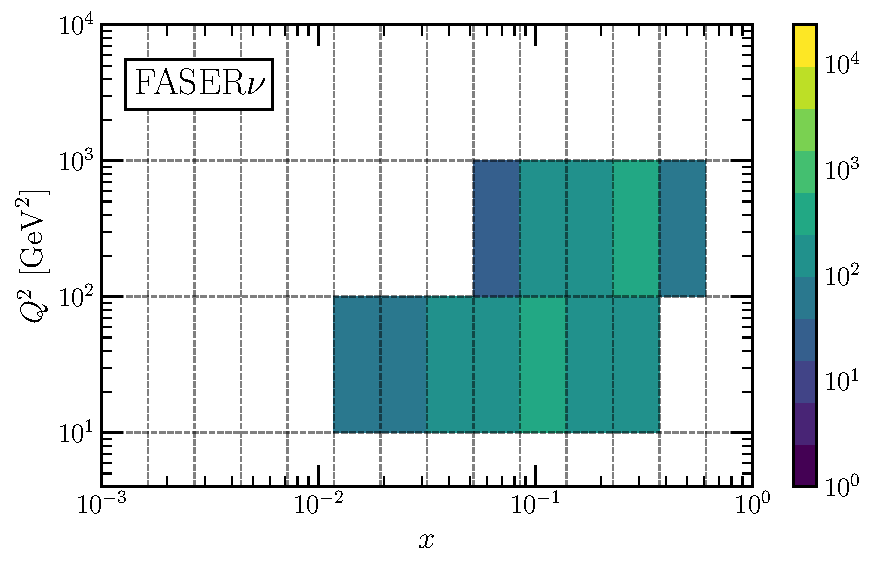
\includegraphics[width=0.495\textwidth]{plots/FPF-FASERv.pdf}
    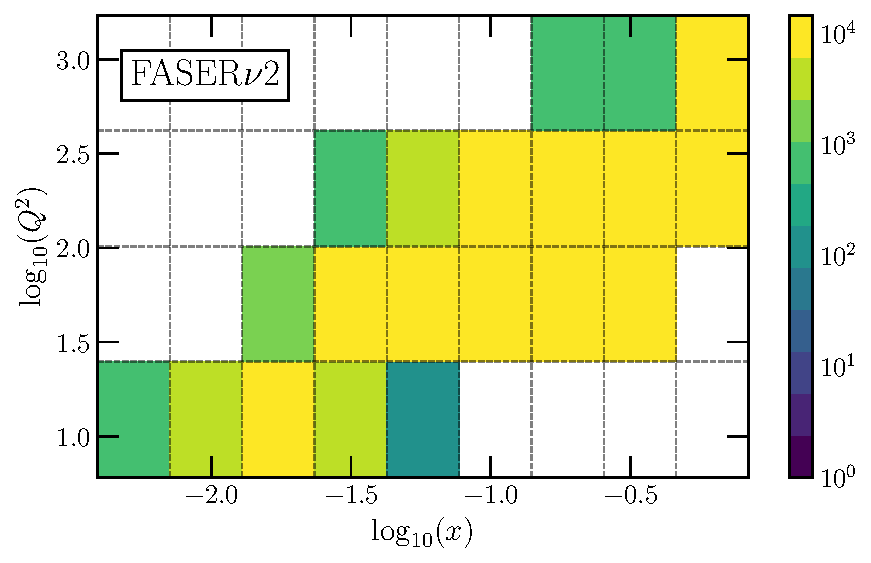
\includegraphics[width=0.495\textwidth]{plots/FPF-FASERv2.pdf}
    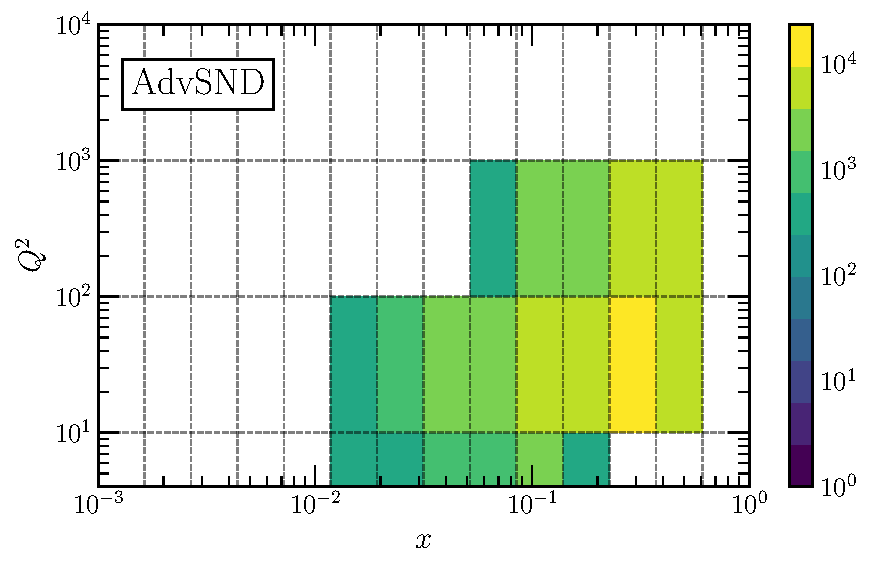
\includegraphics[width=0.495\textwidth]{plots/FPF-AdvSND.pdf}
    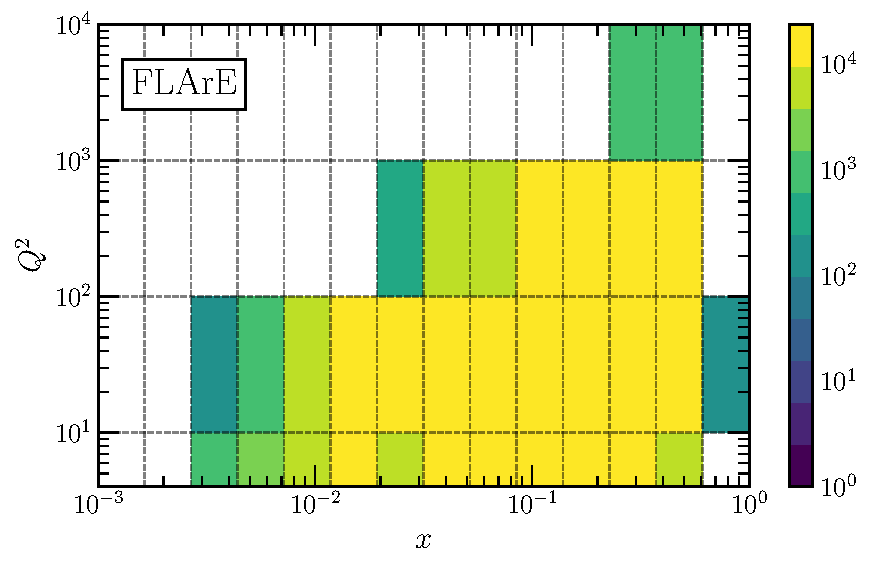
\includegraphics[width=0.495\textwidth]{plots/FPF-FLArE100.pdf}
    \caption{
    	\small The event yields per bin $N_{\rm ev}^{(i)}$,  Eq.~(\ref{eq:event_yields}), for 
    	muon neutrino scattering at the FASER$\nu$, FASER$\nu$2, AdvSND, and FLArE-100  experiments.
        %
   		Selected events are restricted to the DIS region Eq.~(\ref{eq:DISconditions})
   		and only bins with $\ge 100$ events are retained except for FASER$\nu$ in which
   		bins with $\ge 10$ events are kept.
		%
		Adding up the bins in each of the panels results into the numbers listed in
		Table~\ref{tab:integrated_rates}.}
    \label{fig:fasernu2_muon}
\end{figure}
%-----------------------------------------------------------------------

Fig.~\ref{fig:fasernu2_muon} indicates
how the kinematic coverage of the FPF far-forward experiments reaches
$x_{\rm min}\sim 3\times 10^{-3}$ at small-$x$ and $Q^2_{\rm max}\sim 10^4$ GeV$^2$
at large-$Q^2$, representing an extension
of around one order of magnitude in both directions as compared to available
DIS neutrino data on nuclear targets.
%
Fig.~\ref{fig:Kin_nNNPDF30_EIC_FPF} compares
the kinematic coverage of FASER$\nu$, FASER$\nu$2, FLArE, and AdvSND, same as in
Fig.~\ref{fig:fasernu2_muon}, with that of electron-ion collisions
at the upcoming EIC~\cite{Khalek:2021ulf,AbdulKhalek:2021gbh} at the highest
center-of-mass energies planned, as well as to available fixed-target
neutral- and charged-current DIS measurements.
%
The LHC neutrino experiments cover the region $x\gsim 3\times 10^{-3}$, relevant
for precision electroweak measurements at the LHC, such as the $W$-boson
mass, and for new physics measurements sensitive to the large-$x$ quarks
and antiquarks in the proton.
%
FASER$\nu$2 and FLArE-100 mostly overlap with the EIC coverage, providing a complementary handle
on the quark flavour decomposition in protons and heavy nuclei as compared
to that provided by the EIC measurements.

%%%%%%%%%%%%%%%%%%%%%%%%%%%%%%%%%%%%%%%%%%%%%%%%%%%%%
\begin{figure}[t]
    \centering
    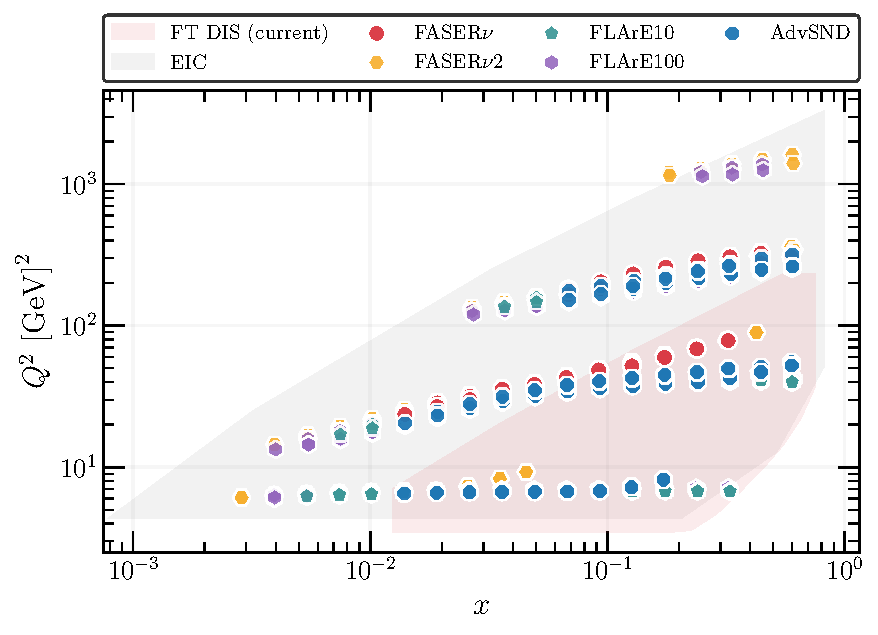
\includegraphics[width = 0.75\textwidth]{plots/KIN_DIS_FPF.pdf}
    \caption{
    	The kinematic coverage in the $(x,Q^2)$ plane of muon-neutrino scattering
	    at the FASER$\nu$, FASER$\nu$2, FLArE-100, and AdvSND experiments, see also Fig.~\ref{fig:fasernu2_muon},
	    compared to that of electron-ion collisions at the EIC for the highest center-of-mass 
	    energies $\sqrt{s}$ planned as well as to the coverage of existing nuclear neutral- and
	    charged-current DIS measurements.
      	%
      	Bins with less than 100 events have been excluded fo all the pseudodata except for FASER$\nu$ where we retain
      	bins with $\ge 10$ events.
  	}
    \label{fig:Kin_nNNPDF30_EIC_FPF}
\end{figure}
%%%%%%%%%%%%%%%%%%%%%%%%%%%%%%%%%%%%%%%%%%%%%%%%%%%%%%%%%%%%%

\subsection{Statistical and systematic uncertainties}
\label{subsec:uncertainties}

The event yields displayed in Fig.~\ref{fig:fasernu2_muon} determine the associated statistical uncertainty 
in each bin,
\be
\label{eq:statistical_uncertainties}
\delta^{\rm (stat)}  N_{\rm ev}^{(i)} = \sqrt{N_{\rm ev}^{(i)}} \, ,
\ee
such that the fractional statistical uncertainty per bin is $\delta^{\rm (stat)}_i=1/\sqrt{N_{\rm ev}^{(i)}}$.
%
Since we discard bins with less than 100 events for HL-LHC experiments (FASER$\nu$2, FLArE100, AdvSND) and
10 events for Run III experiments (FASER$\nu$, SND), the fractional statistical uncertainty
ranges between $\lsim 1\%$ and $\sim 18\%$, depending on the values of
$x$ and $Q^2$ associated to each bin.

%%%%%%%%%%%%%%%%%%%%%%%%%%%%%%%%%%%%%%%%%%%%%%%%%%%%%%%%%%%%%%%%%%%%
\begin{figure}[h]
    \centering
    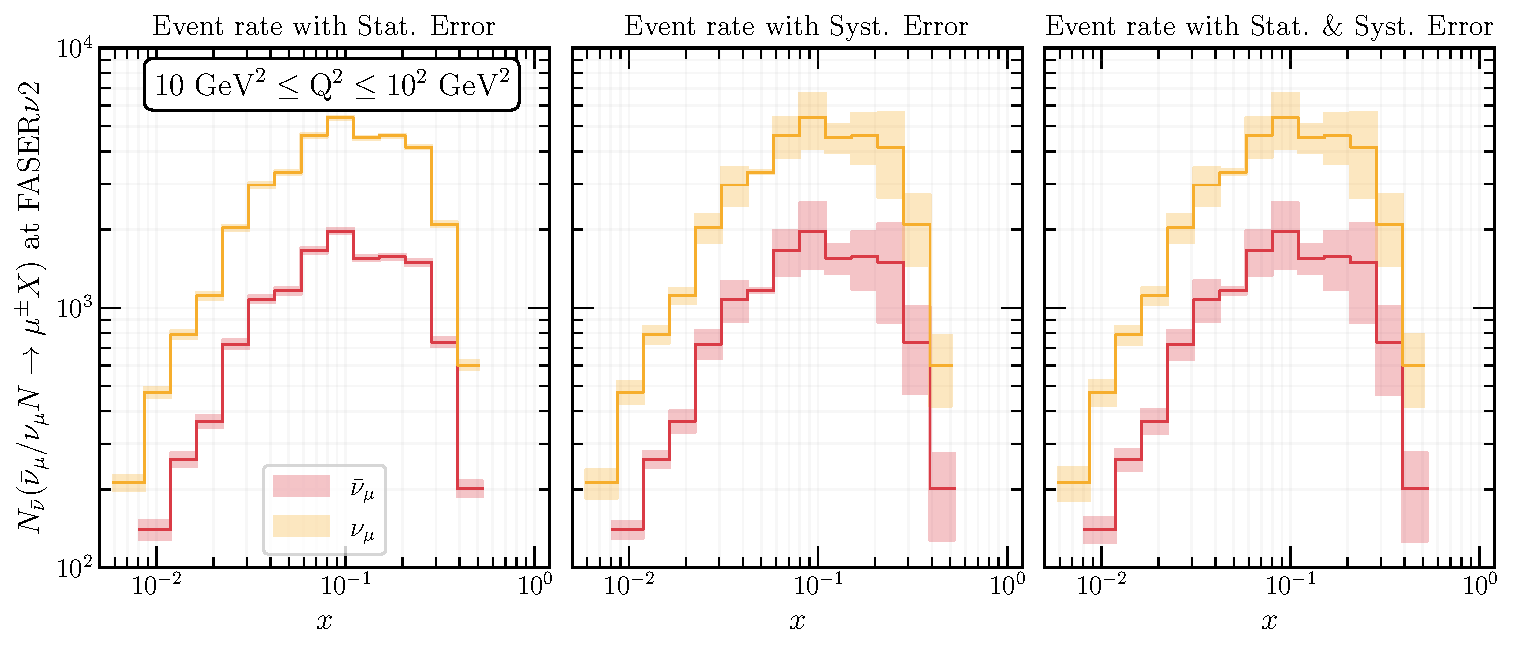
\includegraphics[width = \textwidth]{plots/Event_Rate_FASERv2.pdf}
    \caption{Same as Fig.~\ref{fig:fasernu2_muon} for FASER$\nu$2
      now as a function of $x$ after having integrated the event yields in the range $Q^2 \in [10,100]$ GeV$^2$
      for both the neutrino and antineutrinos.
      %
      In addition to the event yield values, we also show the error bars corresponding to
      statistical errors only (left), systematic errors only (middle), and the
      sum in quadrature of the two (right panel).
      %
      The bars in the horizontal direction indicate the width of the adopted $x$-bins.
      }
    \label{fig:error_plot_FASERv2_14}
\end{figure}
%%%%%%%%%%%%%%%%%%%%%%%%%%%%%%%%%%%%%%%%%%%%%%%%%%%%%%%%%%%%%%%%%%%%

The projected statistical uncertainties for muon-neutrino scattering
in the case of FASER$\nu$2 are displayed in the left panel
of Fig.~\ref{fig:error_plot_FASERv2_14}, which corresponds
to the same event yields as in
Fig.~\ref{fig:fasernu2_muon} for 
now as a function of $x$ after having integrated the event
yields in the range $Q^2 \in [10,100]$ GeV$^2$.
%
The error bar in the vertical direction indicates the statistical uncertainties, while
that in the horizontal direction corresponds to the width of the $x$-bins.
%
Except for the bins with the smallest values of $x$, statistical uncertainties indeed
are at the percent level or smaller for this experiment.

In addition to the statistical uncertainties evaluated from Eq.~(\ref{eq:statistical_uncertainties}),
one needs to also estimate the systematic uncertainties associated to the
finite precision in the reconstruction
of the final state leptonic and hadronic variables listed in Table~\ref{tab:FPF_experiments}.
%
For instance, an event which would be classified into a given bin in $(x,Q^2,E_\nu)$ in the case
of a perfect detector may end up being
mis-classified into a different bin in the presence of systematic
shifts associated to the lepton energy $E_\ell$, lepton scattering angle $\theta_\ell$, and
hadronic energy $E_h$, as indicated by  Eq.~(\ref{eq:dis_kinematic_mapping}).

For each independent source of experimental systematic uncertainty, we hence
quantify its impact at the event yield level.
%
In order to determine these bin-by-bin systematic errors,
we extend the calculation delineated in Eq.~(\ref{sec:pseudo-data_generation}) as follows.
%
Let us consider for illustrative purposes the FASER${\nu}$2 detector.
%
From Table~\ref{tab:FPF_experiments} we know that its
acceptance parameters and reconstruction performance are specified by:
\bea
E_\ell \ge 100~{\rm GeV} \, , \quad \theta_\ell \le \tan^{-1}(0.025)\, , \qquad\\
\delta E_\ell \sim 30\% \, 
 \quad \delta E_h \sim 30\% \, ,
 \quad \delta\theta_\ell \sim 0.06~{\rm mrad} \, . 
\label{eq:fasernu2systematic_errors}
\eea
To translate these uncertainties in $\delta E_\ell$, $\delta E_h $,
and $\delta\theta_\ell$ into systematic errors associated to the event yields, 
\be
\label{eq:event_yields_systematic_error}
\delta_{\rm sys}^{(E_\ell)} N_{\rm ev}^{(i)} \, ,\quad
\delta_{\rm sys}^{(E_h)} N_{\rm ev}^{(i)}
\, ,\quad
\delta_{\rm sys}^{(\theta_\ell)} N_{\rm ev}^{(i)} \, ,\qquad i=1,\ldots,N_{\rm bin} \, ,
\ee
we generate first a Monte Carlo set of events, denoted by $\mathcal{D}_0$,
composed by $N_{\rm mc} \approx 10^7$ samples and determine the assignment of each event
to a point in the $\lp x,Q^2,E_{\nu}\rp$ space.
%
By comparing $\mathcal{D}_0$ with the total number of events as calculated by Eq.~(\ref{MCintegration}), 
we can normalize the distribution to produce the expected yield.

We then produce a second Monte Carlo sample $\mathcal{D}_1$ starting from the events
of $\mathcal{D}_0$ which are then smeared with Gaussian distributions whose variances
are given by Eq.~(\ref{eq:fasernu2systematic_errors}).
%
The bin assignment of the events in the smeared sample $\mathcal{D}_1$ will
in general be different from those of the baseline sample.
%
The procedure is repeated $M$ times, leading to
$\mathcal{D}_k$ (with $k=1,\ldots,M$) smeared
samples each one leading to a different binned event yields
$ N_{\rm ev}^{(i)(k)}$.
%
We take the uncertainty associated
to a given systematic source, say $\delta E_\ell$,
%to be the absolute difference between the mean number of events in this
%bin evaluated for the smeared samples and the
%central prediction for the number of events
to be the mean of the absolute difference between the number of events in this bin for the smeared samples and the central prediction for the number of events
$ N_{\rm ev}^{(i)}$ as calculated from Eq.~(\ref{MCintegration}):
\be
\delta_{\rm sys}^{(E_\ell)} N^{(i)} =\la \Big|  {N}^{(i)}_{E_\ell-{\rm smeared}} -N_{\rm ev}^{(i)}\Big|\ra \, .
\ee

Individual sources of systematic errors are treated as uncorrelated among them and hence
by producing samples where only one source of error is varied at a time
we can determine the systematic errors, Eq.~(\ref{eq:event_yields_systematic_error}), in each bin
for each of the considered experiments.
%
This approach has the benefit that rescaling individual sources of systematic
uncertainties, say to assess the impact of improved detector performance,
becomes straightforward. 

Fig.~\ref{fig:percentage_uncertainties_overview}
displays the projected systematic uncertainties associated
to $E_\ell$, $\theta_\ell$, and $E_h$ 
for the  measurements of the double-differential
muon-neutrino scattering  at FASER$\nu$2.
%
The magnitude of each systematic error is plotted as a function
of the average momentum fraction per bin $\la x\ra$
in two different bins of $Q^2$.
%
We indicate separately the results for neutrino and antineutrino projectiles as well as
those associated to inclusive and to charm production measurements.
%
For completeness, we also display in the bottom-right panel the corresponding
statistical uncertainties in the same bins.

%-----------------------------------------------------------------------
\begin{figure}[t]
  \centering
  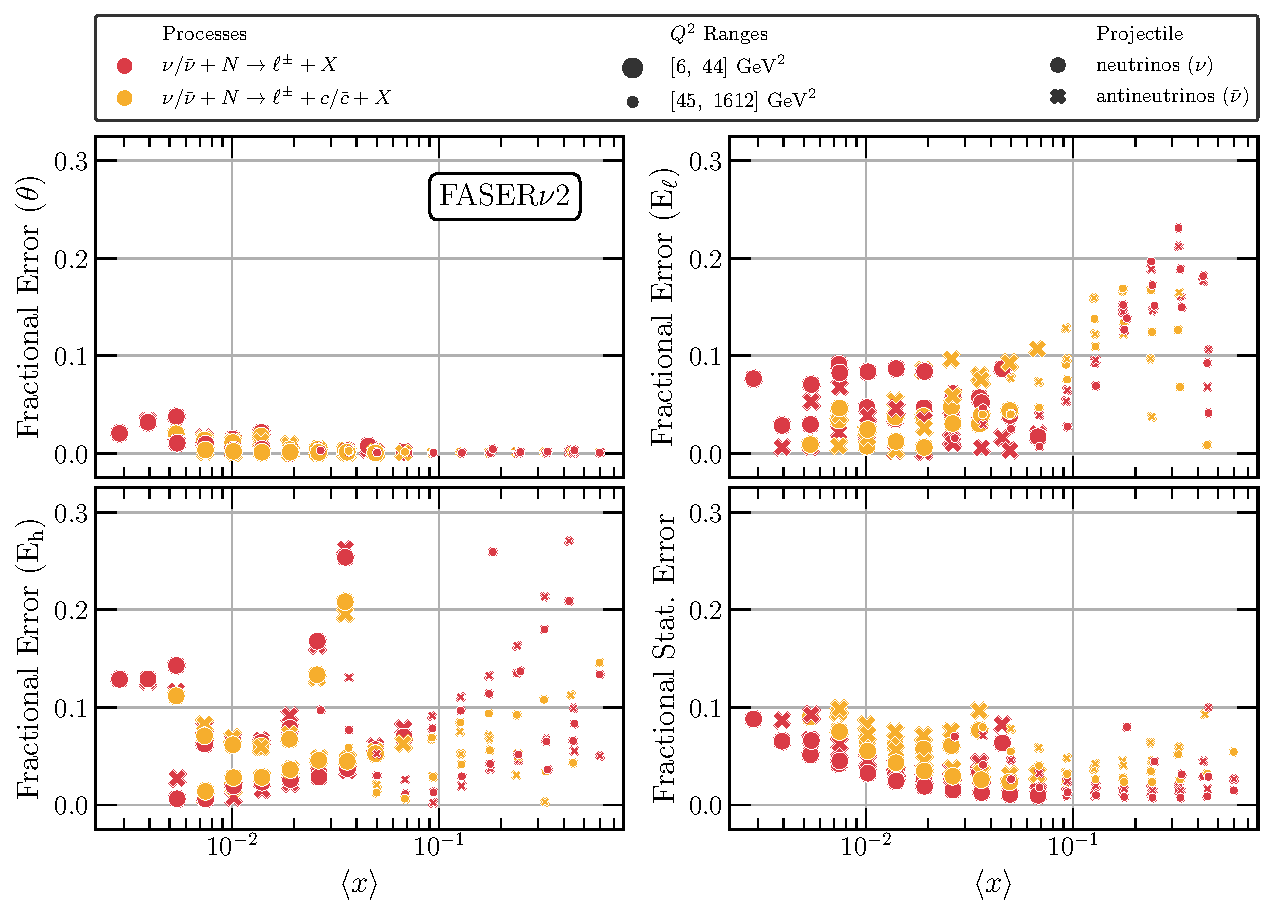
\includegraphics[width=\textwidth]{plots/FASERv2_fractional_error.pdf}
  \caption{\small Estimated systematic uncertainties for the  measurements
    of the double-differential
    muon-neutrino scattering cross-section at FASER$\nu$2.
    %
    We consider the systematic errors
    associated to the charged lepton energy $E_\ell$ and scattering angle $\theta_\ell$
    and to the hadronic energy $E_h$.
    %
    The size of each source of systematic error is plotted as a function
    of the average momentum fraction per bin $\la x\ra$
    in two different bins of $Q^2$.
    %
    We indicate separately the results for neutrino and antineutrino projectiles as well as
    those associated to inclusive and to charm production measurements.
    %
    For completeness, we display in the bottom-right panel the corresponding
    statistical uncertainties in the same bins.
  }
  \label{fig:percentage_uncertainties_overview}
\end{figure}
%-----------------------------------------------------------------------

In general, systematic uncertainties associated to the hadronic final state energy $E_h$ appear to be the largest,
reaching up to $\sim 90\%$ for some experiments.
%
We recall that measurement of $E_h$ in addition to the leptonic variables is required to
fix the incoming neutrino energy $E_\nu$, which is different in each event unlike
the case of neutral-current scattering.
%
The uncertainties associated to the charged-lepton energy $E_\ell$ and scattering angle $\theta_\ell$ range
between a few percent up to 20\% in the  baseline scenario listed in Table~\ref{tab:FPF_experiments}.
%
For the $\delta \theta_\ell$ variations, they are smallest in the large-$x$ region
for $x\gsim 0.1$, where they are at the few-percent level typically.
%
Statistical uncertainties are subdominant in most of the bins and are below the 10\% level,
specially at large-$x$ which is the kinematic region benefitting from the largest event rates.

Fig.~\ref{fig:error_plot_FASERv2_14} also displays
 the integrated event yields for FASER$\nu$2 as a function of $x$ for only
 systematic errors and for the sum in quadrature of statistical and systematic errors
 (central and right panels respectively).
 %
 For most of the bins, for the baseline performance assumptions the total systematic
 uncertainty dominates over the statistical uncertainties, with the possible exception
 of the small-$x$ region where statistical and systematic errors are comparable.

The end result of the procedure is an estimate of statistical and systematic uncertainties
for each bin of the measurement, from which a experimental covariance matrix can be constructed as
\be
\label{eq:covmat_definition}
   {\rm cov}_{ij} = \delta_{ij} \lp \delta^{\rm (stat)}  N_{\rm ev}^{(i)}\rp^2
   + \sum_{k=1}^{n_{\rm sys}}\lp \delta_{\rm sys}^{(k)} N_{\rm ev}^{(i)} \rp \lp \delta_{\rm sys}^{(k)} N_{\rm ev}^{(j)} \rp
   \, ,\qquad i,j=1,\ldots,N_{\rm bin} \, ,
 \ee
  and the same for the associated correlation
 matrix of the measurement
 \be
\label{eq:corrmat_definition}
 \rho_{ij} =  \frac{{\rm cov}_{ij}}{\sqrt{ {\rm cov}_{ii} }\sqrt{ {\rm cov}_{jj} } } \, . 
 \ee
 The relative covariance matrix, $ {\rm cov}_{ij}/( N_{\rm ev}^{(i)}N_{\rm ev}^{(j)})$, is
 independent of the considered observable and would also apply
 for the double-differential cross-sections Eqns.~(\ref{eq:neutrino_DIS_xsec_FL}) and~(\ref{eq:antineutrino_DIS_xsec_FL}) which are related to the event yields by a constant prefactor.
 
 The experimental covariance matrix constructed as per
 Eq.~(\ref{eq:covmat_definition}) assumes that each source of systematic
 uncertainty is 100\% correlated across all the bins of the measurement.
 %
 In the real experiment, the actual covariance matrix will be
 composed by a large number of uncertainty sources, with typical
  HERA and LHC precision measurements characterised by up to hundreds
 of different sources of systematic error.
 %
 In particular, the assumption that a single source of systematic error, say $\delta E_\ell$,
 is fully correlated among all the bins in $(x,Q^2)$ is unlikely to be accurate.
 %
 For this reason, following the HL-LHC projection strategy of~\cite{AbdulKhalek:2018rok}
 here we neglect bin-by-bin correlations
 and add in quadrature statistical and systematic errors,
 \be
\label{eq:covmat_definition_v2}
 {\rm cov}_{ij} = \delta_{ij} \lp \delta^{\rm (stat)}  N_{\rm ev}^{(i)}\rp^2
+ \delta_{ij}\lp f_{\rm corr}\rp^2\sum_{k=1}^{n_{\rm sys}} \lp f_{\rm red}^{(k)}\rp^2\lp \delta_{\rm sys}^{(k)} N_{\rm ev}^{(i)} \rp^2
\, ,\qquad i,j=1,\ldots,N_{\rm bin} \, .
\ee
In Eq.~(\ref{eq:covmat_definition_v2}) we have introduced a parameter $f_{\rm red}^{(k)}\le 1$
that gauges the impact of a possible reduction of the $k$-th systematic error
as compared to the default experiment performance (reproduced with $f_{\rm red}=1$).
%
Furthermore, $f_{\rm corr}$ represents an effective correction factor that accounts for the fact that data with correlated
systematics may be more constraining than the same data where each source of error is simply
added in quadrature as we do here.
%
A value of $f_{\rm corr}=0.5$, obtained from the inspection of available measurements
 for which the full information
 on correlated systematics is available, was estimated in ~\cite{AbdulKhalek:2018rok}
 and we adopt the same choice here.
%
In Sect.~\ref{sec:protonPDFs} we present results for different scenarios
for the systematic uncertainty reduction factor $f_{\rm red}$ with respect to the baseline settings.   
 
 \subsection{Pseudo-data generation}

 In order to generate pseudo-data for double-differential
 LHC neutrino scattering cross-sections, we follow the procedure
 used for the HL-LHC projections of~\cite{AbdulKhalek:2018rok} which was
 also adopted in~\cite{Ethier:2021ydt} and~\cite{Greljo:2021kvv} for SMEFT impact projections
 of vector-boson scattering and high-mass Drell-Yan data at the HL-LHC, respectively.
 %
 The starting point are predictions for inclusive and charm-tagged
 differential neutrino scattering cross-section, denoted generically by
 \be
 \label{eq:theory_dis_projections}
 \mathcal{O}_i^{{\rm (th)}} \equiv \frac{d^2\sigma^{\nu N}(x_i,Q^2_i,y_i)}{dxdy} \, ,\quad
 i=1,\ldots,N_{\rm bin} \, ,
 \ee
 with $(x_i,Q^2_i,y_i)$ labeling the corresponding bin centers.
 %
 The observables $\mathcal{O}_i $ in Eq.~(\ref{eq:theory_dis_projections})
are evaluated with the
{\sc\small YADISM}~\cite{yadism,Candido:2023utz} program
interfaced to {\sc\small PineAPPL}~\cite{Carrazza:2020gss, christopher_schwan_2023_7995675}
to return a fast interpolation grid admitting a generic PDF input,
and with DGLAP evolution effects provided by {\sc\small EKO}~\cite{Candido:2022tld}.
%
PDF evolution and DIS structure functions account for NLO QCD corrections
and target mass effects.
%
No higher-twists corrections are included.
%
Charm structure functions are evaluated in the FONLL general-mass variable-flavour-number
scheme~\cite{Forte:2010ta,Ball:2011mu,Faura:2020oom} at $\mathcal{O}\lp \alpha_s\rp$
accuracy.
%
For the proton PDF fits we assume a free isoscalar target $N$, while
for the nuclear PDF one we allow for deviations from isoscalarity relevant
for a tungsten nucleus.

The PDF set and other theory settings, such as the perturbative
order and heavy quark scheme, adopted for the evaluation of
Eq.~(\ref{eq:theory_dis_projections}) should be the same as those
used in the fitting framework assessing their impact.
%
For instance, when using the {\sc\small xFitter} profiling of PDF4LHC21, one needs
 to generate LHC neutrino pseudo-data also using PDF4LHC21 as input.
 %
This ensures that the generated pseudo-data is consistent with the prior PDF
 set used as baseline and avoids introducing artificial inconsistencies 
 compromising the validity of the projection studies.
 
 The central values for the pseudo-data, denoted
 by $\mathcal{O}_i^{{\rm (exp)}} $, are obtained
 by fluctuating the reference theory prediction Eq.~(\ref{eq:theory_dis_projections})
 by the corresponding fractional statistical and systematic
 uncertainties,
 \begin{equation}
  \label{eq:pseudo_data_v2}
  \mathcal{O}_i^{{\rm (exp)}}
  = \mathcal{O}_i^{{\rm (th)}}
    \left( 1+ r_i \delta_i^{\rm tot}
    \right) \,
    , \qquad i=1,\ldots,N_{\rm bin} \, ,
 \end{equation}
 where the total experimental uncertainty is the sum in quadrature of
 statistical and systematic errors, accounting for a possible reduction
 factor in the latter,
  \be
 \delta_{i}^{\rm tot}
 = \left( \left( \delta_i^{\rm stat}\right)^2 + \sum_{k=1}^{n_{\rm sys}}
 \left( f_{\rm corr} \times f_{\rm red}^{(k)} \times \delta_{i,k}^{\rm sys} \right)^2\right)^{1/2} \, ,
 \qquad i=1,\ldots,N_{\rm bin} \, ,
 \ee
 and with $r_{i}$ being univariate Gaussian random numbers. 
 %
 As mentioned above, $f_{\rm red}^{(k)}$ is a reduction factor modelling
 improvements in the experimental performance as compared to the baseline
 settings summarised in Sect.~\ref{tab:FPF_experiments}.
 %
 Here we consider two scenarios for the systematic errors: ``conservative'',  with $f_{\rm red}=1$, where
 no improvement as compared to current projected performance takes place, and ``optimistic'', with  $f_{\rm red}=0.5$, a factor
 two improvement for all sources of systematics.
 %
 The pseudo-data generated by means of Eq.~(\ref{eq:pseudo_data_v2}),
 together with the corresponding covariance matrix computed according to Eq.~\eqref{eq:covmat_definition_v2},
 define then the inputs of the subsequent proton and nuclear PDF determination.

 \subsection{PDF impact assessment}
 \label{subsec:pdf_impact_assessment}

We consider two complementary approaches to assess the
impact of the projected LHC neutrino data on the proton and nuclear PDFs.
%
First, the Hessian profiling\cite{Paukkunen:2014zia, Schmidt:2018hvu, AbdulKhalek:2018rok, HERAFitterdevelopersTeam:2015cre} of prior proton and
nuclear PDF sets, taken to be PDF4LHC21~\cite{PDF4LHCWorkingGroup:2022cjn} and
EPPS21~\cite{Eskola:2021nhw} respectively.
%
Second, the direct inclusion 
in the NNPDF global analysis framework~\cite{NNPDF:2021uiq,NNPDF:2021njg}.
%
The profiling method applied to Hessian PDF fits is based
on minimizing a goodness-of-fit error function defined as
\begin{equation}
\chi^2 = 
\sum_{i=1}^{N_{\textrm{bin}}} 
\frac{\left(  \mathcal{O}_i^{\rm (exp)}
            + \Gamma_i^{\alpha,\textrm{exp}}
              b_\alpha^{\textrm{(exp)}}
            - \mathcal{O}_i^{\rm (th)}
            - \Gamma_i^{\beta,\textrm{th}}
              b_\beta^{(\textrm{th})}
     \right)^2
     }{ \left(\delta^{{\rm (stat)}}\mathcal{O}_i^{\rm (th)}\rp^2 }
+ \sum_\alpha \lp b_\alpha^{(\textrm{exp})}\rp^2
+ T^2 \sum_\beta  \lp b_\beta^{\textrm{(th)}}\rp ^2 \, ,
\label{eq:profilingchi2}
\end{equation}
with the pseudodata 
$\mathcal{O}_i^{\rm (exp)}$ defined in  Eq.~(\ref{eq:pseudo_data_v2}).
%
The correlated uncertainties for the pseudodata and for the theoretical prediction 
are contained in the nuisance parameter vectors $b^{(\textrm{exp})}$ and $b^{(\textrm{th})}$, respectively, with $T$ the tolerance factor, and the total uncorrelated uncertainty is $\delta^{{\rm (stat)}}\mathcal{O}_i^{\rm (th)}$.

The effect of the nuisance parameters
on the observables $\mathcal{O}_i^{\rm (exp)}$ and $\mathcal{O}_i^{\rm (th)}$
is described by the matrices $\Gamma_i^{\textrm{exp}}$ and $\Gamma_i^{\textrm{th}}$.
%
The indices $\alpha$ and $\beta$ then run over the uncertainty nuisance parameters for the pseudodata and the theoretical prediction, respectively.
%
The nuisance parameter values $b_\beta^{\textrm{(th,min)}}$ that minimize Eq.~\eqref{eq:profilingchi2} give the central PDFs $f'_0$ optimized to the profiled dataset in the form
\begin{equation}
f_0' = f_0
      + \sum_\beta b_\beta^{\textrm{(th,min)}} 
        \left(  \frac{f_\beta^+   -  f_\beta^- }{2}
              -    b_\beta^{\textrm{(th,min)}}
                \frac{f_\beta^+ + f_\beta^- - 2f_0}{2}
        \right),
\end{equation}
where $f_0$ is the original central PDF and the up and down variation eigenvectors are given by $f^+, f^-$.
%
The reduction in the uncertainties of the profiled PDFs indicate the impact
of the projected data with respect to the assumed prior PDF set.

The profiling studies carried out in this work are performed using version 2.2.1
of the 
{\sc\small xFitter} open-source QCD analysis framework~\cite{Alekhin:2014irh, Bertone:2017tig, xFitter:2022zjb, xFitter:web}.
%
To this end, a new interface between  {\sc\small PineAPPL} and {\sc\small xFitter} has been developed and is available in {\sc\small xFitter}.
%
All the experimental and theoretical data files used in the analysis, including
the  {\sc\small PineAPPL}  grids, are available
from the {\sc\small xFitter} repository.
%
For the proton PDF profiling, a tolerance of $T^2 = 10$ is adopted,
which  corresponds approximately to the average tolerance
used in the CT18~\cite{Hou:2019efy} and MSHT20~\cite{Bailey:2020ooq} determinations,
the two Hessian sets entering the PDF4LHC21 combination~\cite{PDF4LHCWorkingGroup:2022cjn}, for
one-sigma PDF uncertainties.
%
For the Hessian profiling of EPPS21, a value of $T^2 = 20$ is used consistently with~\cite{Eskola:2021nhw}
for the definition of 68\%  confidence level intervals.

Concerning the inclusion of the LHC far-forward neutrino pseudo-data
in the NNPDF proton analysis framework, we follow the procedure
outlined in~\cite{NNPDF:2021uiq}.
%
Fast interpolation tables (FK-tables)~\cite{Ball:2010de} combining {\sc\small EKO}
DGLAP evolution with {\sc\small YADISM} DIS coefficient functions
are computed using {\sc\small PineAPPL}, see also~\cite{Barontini:2023vmr}.
%
Predictions for the observables Eq.~(\ref{eq:theory_dis_projections}) are evaluated
with NNPDF4.0 NNLO for various choices of input datasets, and included
directly in the same alongside all other datasets in the global fit.
%
We verify that in all cases $\chi^2/n_{\rm dat}\sim 1$ after the fit,
as expected given the built-in consistency between the prior PDF fit
and the generated pseudo-data.
%
We assess the impact of the forward LHC neutrino data in the NNPDF fits both when added
on top of the baseline dataset and when added to a dataset which excludes previous neutrino DIS
cross-section measurements.





\section{Constraints on proton and nuclear structure}
\label{sec:protonPDFs}

By following the strategy outlined in Sect.~\ref{sec:dis_pseudodata}, one can
quantify the impact on the proton and nuclear PDFs of differential  DIS
cross-section measurements exploiting the  LHC neutrino beam. 
%
We present results first for the Hessian profiling of the PDF4LHC21,
then for the Monte Carlo fit NNPDF4.0, and finally for the nuclear PDFs of EPPS21, also
by means of profiling.
%
We study the stability of the results with respect to the inclusion of systematic uncertainties,
charm-tagged data, and lepton-charge separation.
%
We also compare the impact of the different FPF experiments separately and provide
results for their combination.

\subsection{Proton PDFs: impact on PDF4LHC21}
\label{sec:pdf4lhc21}

We begin by presenting results for the Hessian profiling of
the PDF4LHC21 set.
%
This proton PDF set is a Monte Carlo combination~\cite{Watt:2012tq,Carrazza:2015hva} of three global PDF sets, CT18~\cite{Hou:2019efy},
MSHT20~\cite{Bailey:2020ooq}, and NNPDF3.1~\cite{NNPDF:2017mvq}.
%
Its Hessian representations are obtained by means of the reduction methodologies developed in~\cite{Gao:2013bia,Carrazza:2015aoa}.
%
Being based on the combination of three modern global PDF fits, PDF4LHC21 provides a robust estimate
of  current uncertainties associated to our understanding of proton PDFs.
%
We profile PDF4LHC21 with pseudodata from various LHC neutrino experiments,
and study the stability of the results with respect to variations in the profiling inputs.

%%%%%%%%%%%%%%%%%%%%%%%%%%%%%%%%%%%%%%%%%%%%%%%%%%%%%%%%%%%%%%%%%%%%%%%%
\begin{figure}[t]
\centering
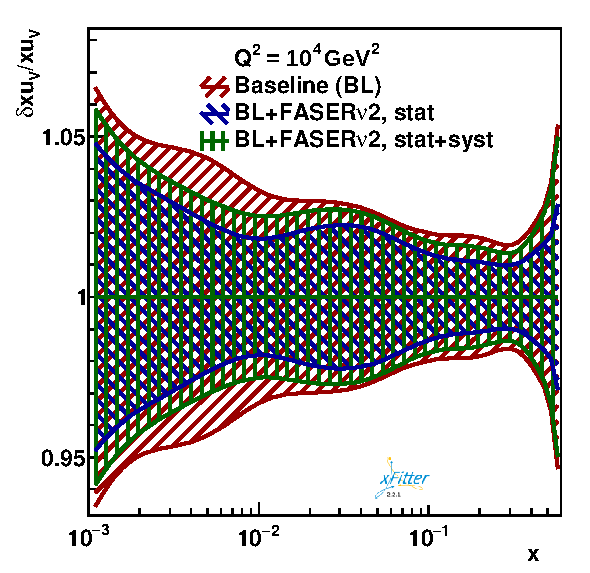
\includegraphics[width=0.32\textwidth]{plots/proton_fasernu2/inclusive+charm_chargediscrimination/fred05fcorr05_FASERv2_q2_10000_pdf_uv_ratio.pdf}
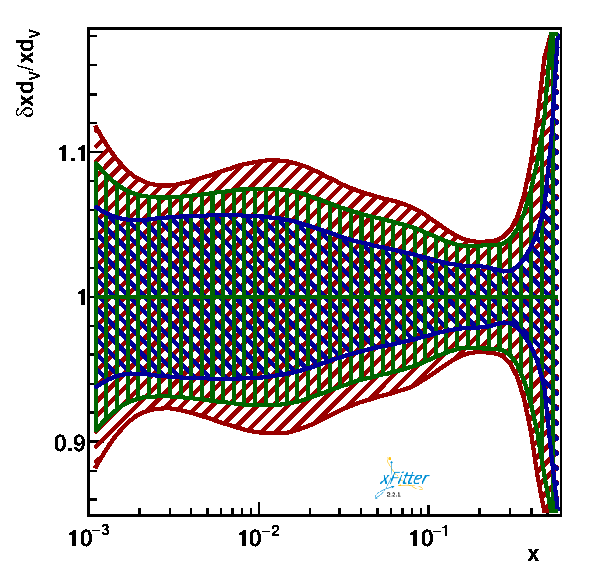
\includegraphics[width=0.32\textwidth]{plots/proton_fasernu2/inclusive+charm_chargediscrimination/fred05fcorr05_FASERv2_q2_10000_pdf_dv_ratio.pdf}
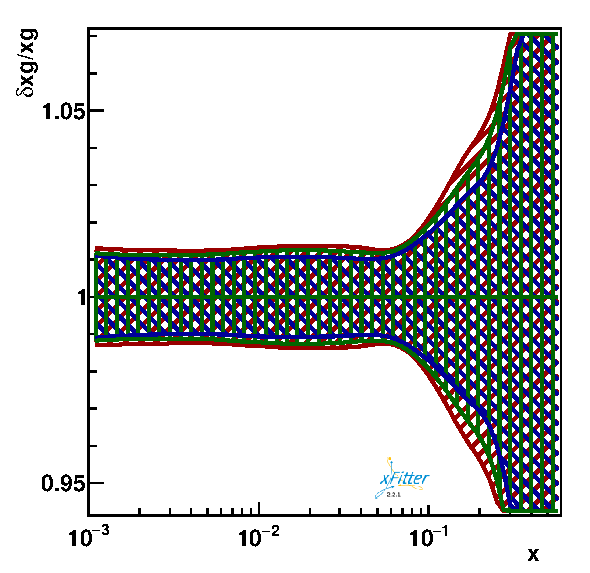
\includegraphics[width=0.32\textwidth]{plots/proton_fasernu2/inclusive+charm_chargediscrimination/fred05fcorr05_FASERv2_q2_10000_pdf_g_ratio.pdf}\\
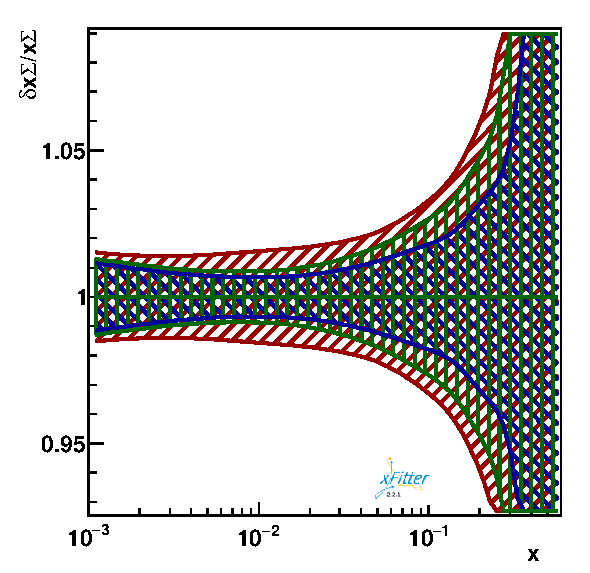
\includegraphics[width=0.32\textwidth]{plots/proton_fasernu2/inclusive+charm_chargediscrimination/fred05fcorr05_FASERv2_q2_10000_pdf_Sea_ratio.pdf}
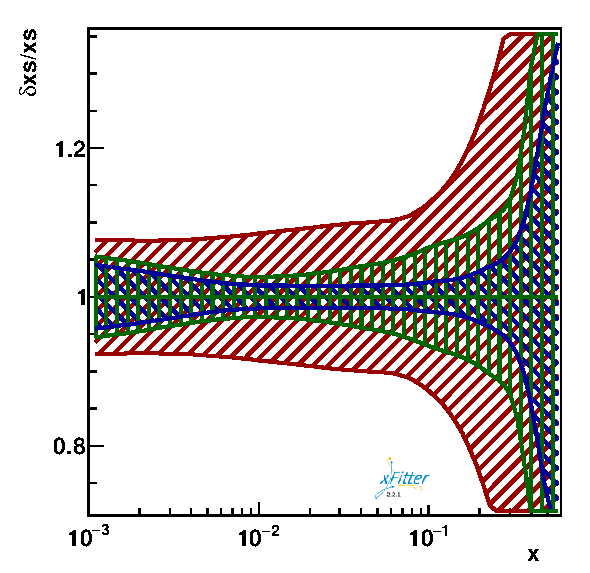
\includegraphics[width=0.32\textwidth]{plots/proton_fasernu2/inclusive+charm_chargediscrimination/fred05fcorr05_FASERv2_q2_10000_pdf_s_ratio.pdf}
\caption{
The fractional PDF uncertainties (at the 68\% confidence level) at $Q^2 = 10^4 \, \textrm{GeV}^2$ 
for the up and down valence quarks, gluon, total quark singlet, and total strangeness PDFs
in the PDF4LHC21 baseline, compared to the results obtained once the FASER$\nu$2 structure
functions are included.
%
The FASER$\nu$2 impact projections are presented both without and with systematic
uncertainties accounted for, and include charm-tagged structure functions
as well as final-state lepton-charge separation.
%
}
\label{fig:FASERnu2_baseline}
\end{figure}
%%%%%%%%%%%%%%%%%%%%%%%%%%%%%%%%%%%%%%%%%%%%%%%%%%%%%%%%%%%%%%%%%%%%%%%%

\paragraph{Constraints from FASER$\nu$2.}
%
Fig.~\ref{fig:FASERnu2_baseline} shows the
fractional uncertainties (at the 68\% confidence level) at $Q^2 = 10^4 \, \textrm{GeV}^2$ 
for the up and down valence quarks, gluon, total quark singlet, and total strangeness PDFs
in the PDF4LHC21 baseline, compared to the results obtained once the FASER$\nu$2 structure functions are
added by means of Hessian profiling.
%
The FASER$\nu$2 pseudo-data accounts for  both  inclusive and charm-tagged structure functions
and assumes outgoing lepton- charge identification.
%
We display results for the profiling in which the experimental covariance matrix
considers only statistical uncertainties, as well as for the scenario where
statistical and systematic errors are added in quadrature following
the procedure spelled out in Sect.~\ref{subsec:uncertainties}.
%
We restrict the comparisons to the region $10^{-3}\lsim x \lsim 0.7$ covered
by the LHC neutrino experiments (see Fig.~\ref{fig:Kin_nNNPDF30_EIC_FPF}).
%
In addition of a reduction of PDF uncertainties, the Hessian profiling
also results in general in a shift in the PDF central values.
%
This shift is however arbitrary since it 
depends on the fluctuations
entering the pseudo-data generation, and is hence ignored in the following.

Inspection of Fig.~\ref{fig:FASERnu2_baseline} reveals that measurements of DIS structure
functions at FASER$\nu$2 improve PDF uncertainties on the quark PDFs, while leaving
the gluon essentially unaffected.
%
As expected for a neutrino scattering experiment, its impact is most marked for
those PDF combinations sensitive to quark flavour separation such as
the up and down valence PDF as well as the total strangeness.
%
Indeed, the reduction of PDF uncertainties is particularly significant for the latter,
a consequence of the inclusion of charm-tagged structure functions in the fit.
%
Given that all PDF determinations entering PDF4LHC21 already include existing neutrino
DIS measurements, the fact that FASER$\nu$2 pseudo-data still manages to reduce PDF
uncertainties highlights the new information provided by the LHC neutrino experiments.

By comparing the impact of the FASER$\nu$2 structure functions
in the case where only statistical errors are considered with that
where also systematic uncertainties are accounted for,
one finds that the latter eventually become a limiting factor,
but also that they not modify the qualitative findings of the statistics-only scenario.
%
Indeed, while systematic uncertainties somewhat degrade the PDF sensitivity,
they don't eliminate it for none of the quark PDFs.
%
Furthermore, in the projections presented in this work,
we assume the performance parameters of  Table~\ref{tab:FPF_experiments}, which
however could be very well enhanced in the actual realisation of the experiments,
using for instance detector improvements or different kinematic reconstruction techniques.
%
We also note that the availability of different experiments accessing the same neutrino
beam should allow their mutual cross-calibration, such that the combination of their
data brings in more information than just the trivial statistics scaling.

\paragraph{Importance of charm-tagged measurements.}
%
The analysis of Fig.~\ref{fig:FASERnu2_baseline} highlights that LHC neutrino data is particularly
constraining for the poorly-known strange PDF, which is one of the quark flavour combinations
for which proton PDF fits differ the most~\cite{Faura:2020oom}.
%
To further investigate this point, Fig.~\ref{fig:FASERnu2_nocharm} compares the impact of the FASER$\nu$2 data shown in
Fig.~\ref{fig:FASERnu2_baseline}, for the case in which only statistical
uncertainties are considered, with the results of the same profiling once the charm-tagged
structure function data is excluded from the fit.
%
While differences are moderate for the up and down quark PDFs, the significant loss
of information resulting from this exclusion of charm-tagged data is clearly
visible for the strange PDF.
%
Specially in the region $x\gsim 0.01$, the constraints on strangeness shown in
Fig.~\ref{fig:FASERnu2_nocharm} are washed out in the absence of charm-tagged data.
%
We thus establish that inclusive neutrino DIS measurements constrain mostly
the up and down quark and antiquark PDFs (and thus also the quark singlet), while the charm-tagged
structure functions are responsible for most of the constraints provided on the total strangeness.
%
The PDF reach of the LHC neutrino experiments would thus be  markedly limited in experiments without
charm-identification capabilities.

%%%%%%%%%%%%%%%%%%%%%%%%%%%%%%%%%%%%%%%%%%%%%%%%%%%%%%%%%%%%%%%%%%%%%%%%
\begin{figure}[t]
\centering
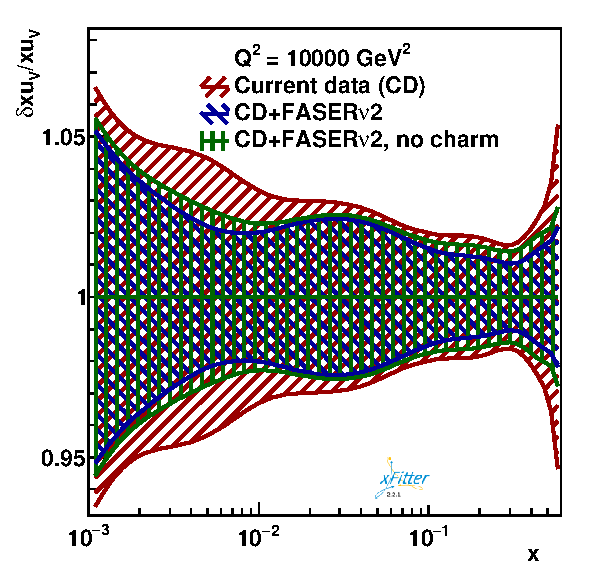
\includegraphics[width=0.32\textwidth]{plots/proton_fasernu2/inclusive-only_vs_inclusive+charm/statOnly_FASERv2_q2_10000_pdf_uv_ratio.pdf}
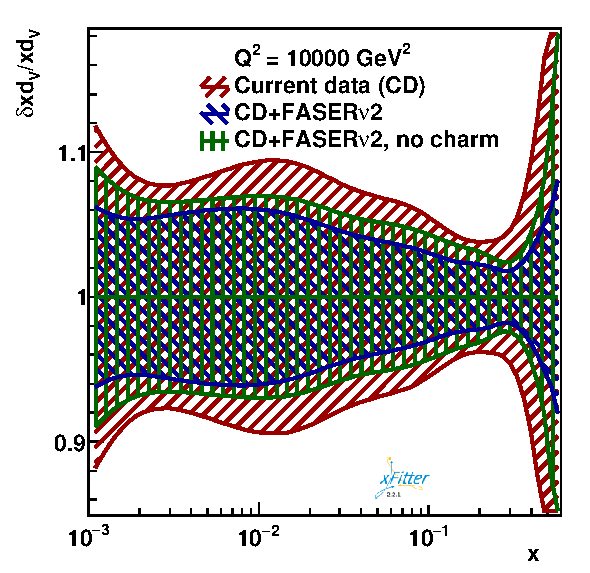
\includegraphics[width=0.32\textwidth]{plots/proton_fasernu2/inclusive-only_vs_inclusive+charm/statOnly_FASERv2_q2_10000_pdf_dv_ratio.pdf}
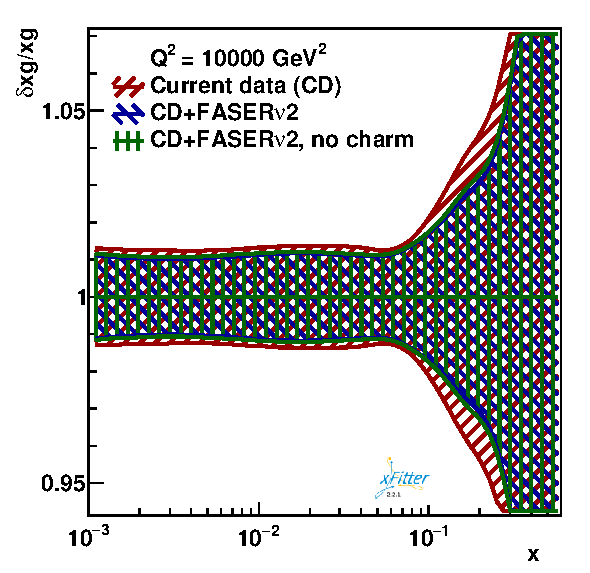
\includegraphics[width=0.32\textwidth]{plots/proton_fasernu2/inclusive-only_vs_inclusive+charm/statOnly_FASERv2_q2_10000_pdf_g_ratio.pdf}\\
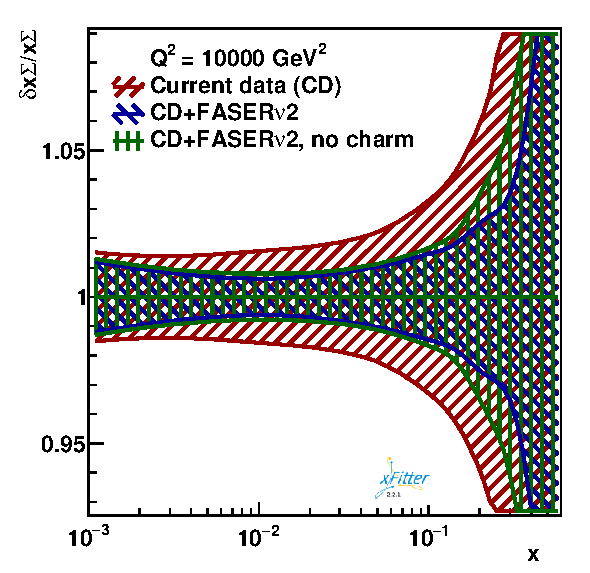
\includegraphics[width=0.32\textwidth]{plots/proton_fasernu2/inclusive-only_vs_inclusive+charm/statOnly_FASERv2_q2_10000_pdf_Sea_ratio.pdf}
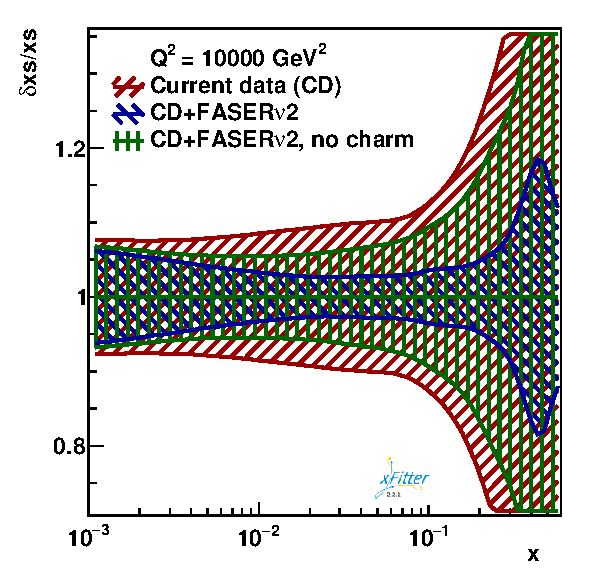
\includegraphics[width=0.32\textwidth]{plots/proton_fasernu2/inclusive-only_vs_inclusive+charm/statOnly_FASERv2_q2_10000_pdf_s_ratio.pdf}
\caption{Same as Fig.~\ref{fig:FASERnu2_baseline} (statistical uncertainties only),
  now showing results in the scenario where charm-tagged structure function measurements
  are excluded from the analysis.
}
\label{fig:FASERnu2_nocharm}
\end{figure}
%%%%%%%%%%%%%%%%%%%%%%%%%%%%%%%%%%%%%%%%%%%%%%%%%%%%%%%%%%%%%%%%%%%%%%%%

\paragraph{Lepton-charge identification.}
%
Being able to identify the charge of the produced final-state lepton in charged-current
neutrino scattering demands equipping an experiment with a powerful enough magnet suitable to
deflect this lepton within the detector fiducial volume.
%
Our baseline results for FASER$\nu$2 in Fig.~\ref{fig:FASERnu2_baseline} assume that this charge-identification
is possible, and therefore include separate structure function datasets for neutrino and anti-neutrino projectiles.
%
In order to ascertain to which extent the constraints provided by FASER$\nu$2 structure functions
depend on the availability of such a magnet,
Fig.~\ref{fig:FASERnu2_nochargeID} compares the reduction of the PDF uncertainties using
the FASER$\nu$2 data with and without charged-lepton identification capabilities.

%%%%%%%%%%%%%%%%%%%%%%%%%%%%%%%%%%%%%%%%%%%%%%%%%%%%%%%%%%%%%%%%%%%%%%%%
\begin{figure}[t]
\centering
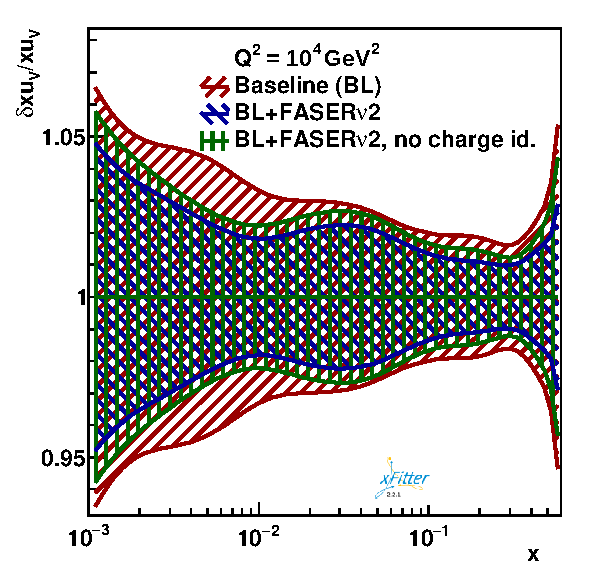
\includegraphics[width=0.32\textwidth]{plots/proton_fasernu2/nochargediscrimination/statOnly_FASERv2_q2_10000_pdf_uv_ratio.pdf}
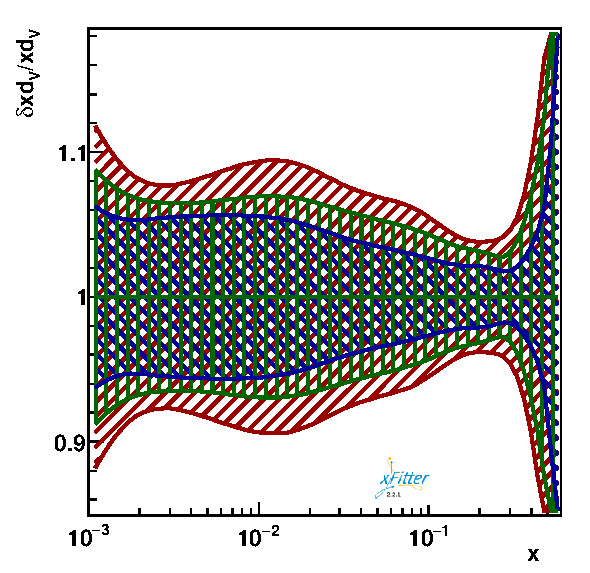
\includegraphics[width=0.32\textwidth]{plots/proton_fasernu2/nochargediscrimination/statOnly_FASERv2_q2_10000_pdf_dv_ratio.pdf}
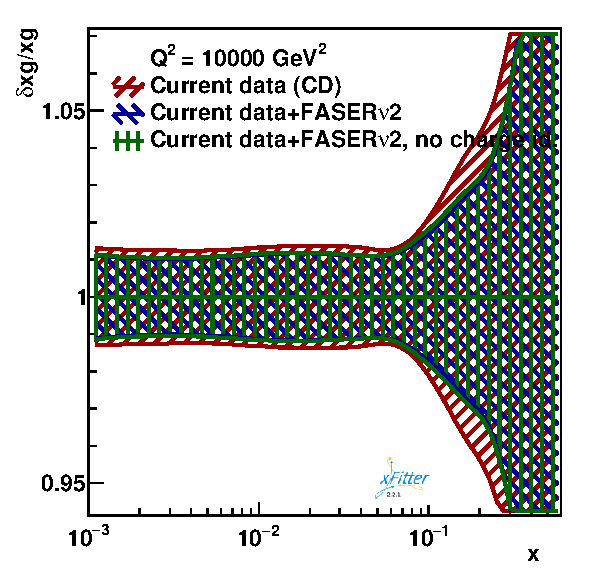
\includegraphics[width=0.32\textwidth]{plots/proton_fasernu2/nochargediscrimination/statOnly_FASERv2_q2_10000_pdf_g_ratio.pdf}\\
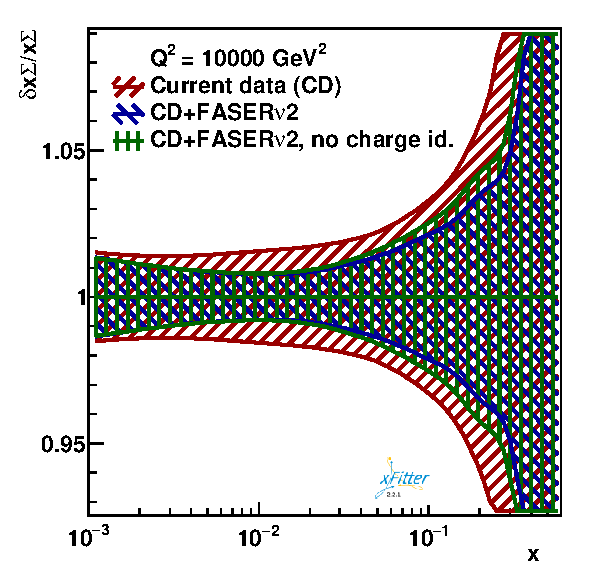
\includegraphics[width=0.32\textwidth]{plots/proton_fasernu2/nochargediscrimination/statOnly_FASERv2_q2_10000_pdf_Sea_ratio.pdf}
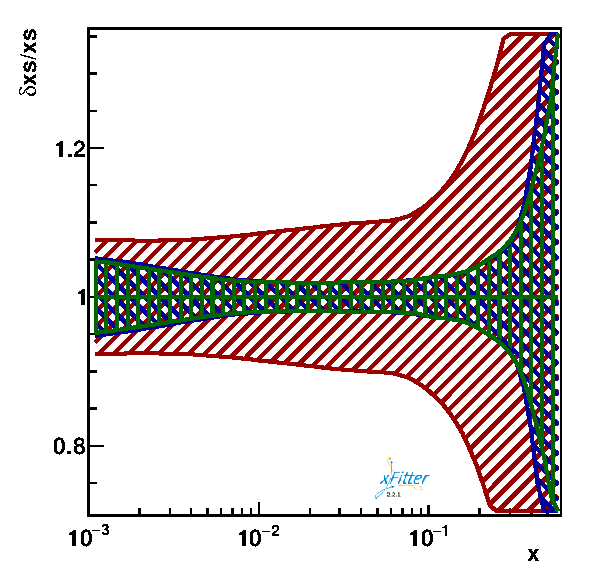
\includegraphics[width=0.32\textwidth]{plots/proton_fasernu2/nochargediscrimination/statOnly_FASERv2_q2_10000_pdf_s_ratio.pdf}
\caption{Same as Fig.~\ref{fig:FASERnu2_baseline} (statistical uncertainties only),
  now showing results in the scenario where the charge of the final-state charged lepton
  cannot be identified.
 }
\label{fig:FASERnu2_nochargeID}
\end{figure}
%%%%%%%%%%%%%%%%%%%%%%%%%%%%%%%%%%%%%%%%%%%%%%%%%%%%%%%%%%%%%%%%%%%%%%%%

This analysis finds that the lack of charged-lepton identification actually does not degrade significantly the PDF
sensitivity of FASER$\nu$2.
%
Having access of the lepton charge information improves a bit the constraints for the down and (to a lesser
extent) the up valence quark PDFs,  while there are no differences for the total quark
singlet and for strangeness.
%
This behaviour can be understood by inspecting the leading-order decomposition of neutrino DIS
structure functions in terms of PDFs for different targets, Eqns.~(\ref{eq:neutrinoSFs_proton})--(\ref{eq:neutrinoSFs_isoscalar}).
%
For an isoscalar target, as assumed here, structure functions are very similar for neutrino
and anti-neutrino projectiles, with differences restricted to the strangeness asymmetry.
%
Given that this strangeness asymmetry is quite small, this also explains why the impact
on strangeness, which is driven by the charm-tagged data, is the same irrespective of whether one identifies
the outgoing lepton charge.
%
We conclude that LHC neutrino DIS data exhibits good PDF sensitivity even for detectors which cannot
separate incoming neutrinos from antineutrinos.

\paragraph{Experiment dependence.}
%
In addition to FASER$\nu$2, we have also produced PDF impact projections for
other proposed FPF experiments, specifically for AdvSND and FLArE.
%
In the latter case, we consider both the 10 ton and 100 ton variants.
%
Fig.~\ref{fig:FASERnu2_FLAre10} compares the PDF sensitivity
of FASER$\nu$2, in the scenario where systematic uncertainties are neglected, with the corresponding
results for AdvSND and FLArE10 respectively.
%
As summarised by Table~\ref{tab:integrated_rates}, each of these experiments
has associated different expected numbers of DIS events, namely 260k, 28k, and 57k (340k)
inclusive muon-neutrino events for FASER$\nu$2, AdvSND and FLArE10~(100) respectively,
with 39k, 3.5k, and 7.7k (45k) in the charm-tagged case.
%
As shown below, experiments with the largest event rates are those exhibiting the
best PDF sensitivity.

%%%%%%%%%%%%%%%%%%%%%%%%%%%%%%%%%%%%%%%%%%%%%%%%%%%%%%%%%%%%%%%%%%%%%%%%
\begin{figure}[htbp]
\centering
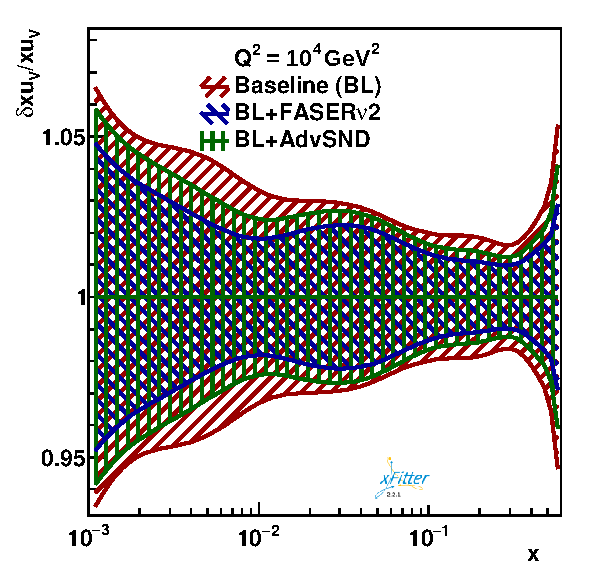
\includegraphics[width=0.32\textwidth]{plots/proton_fasernu2/FASERv2_vs_AdvSND/statOnly_AdvSND_q2_10000_pdf_uv_ratio.pdf}
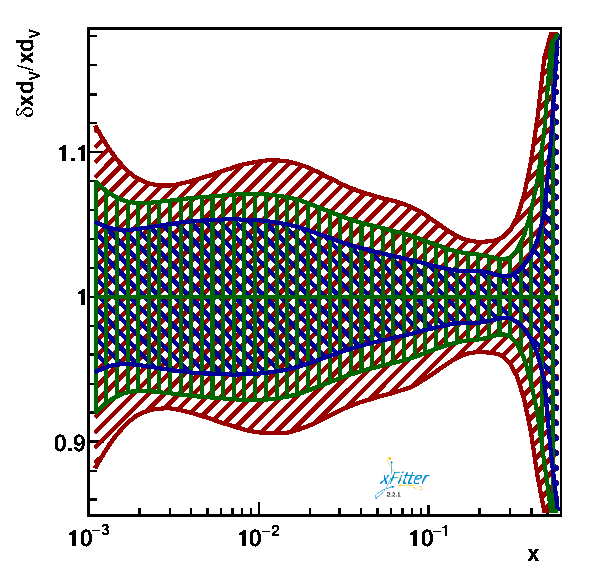
\includegraphics[width=0.32\textwidth]{plots/proton_fasernu2/FASERv2_vs_AdvSND/statOnly_AdvSND_q2_10000_pdf_dv_ratio.pdf}
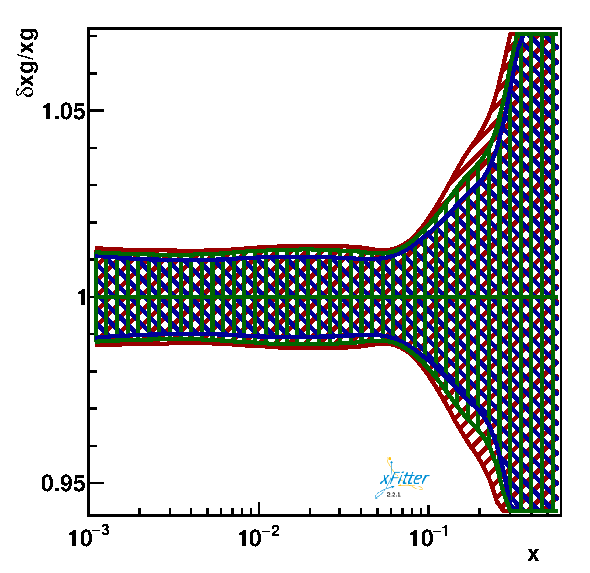
\includegraphics[width=0.32\textwidth]{plots/proton_fasernu2/FASERv2_vs_AdvSND/statOnly_AdvSND_q2_10000_pdf_g_ratio.pdf}\\
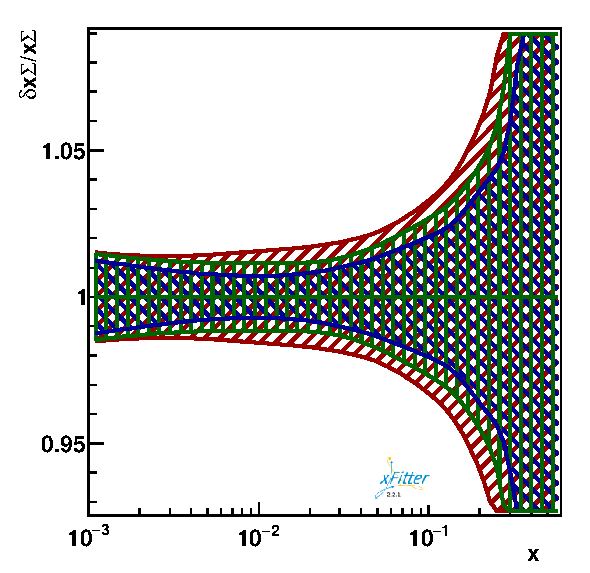
\includegraphics[width=0.32\textwidth]{plots/proton_fasernu2/FASERv2_vs_AdvSND/statOnly_AdvSND_q2_10000_pdf_Sea_ratio.pdf}
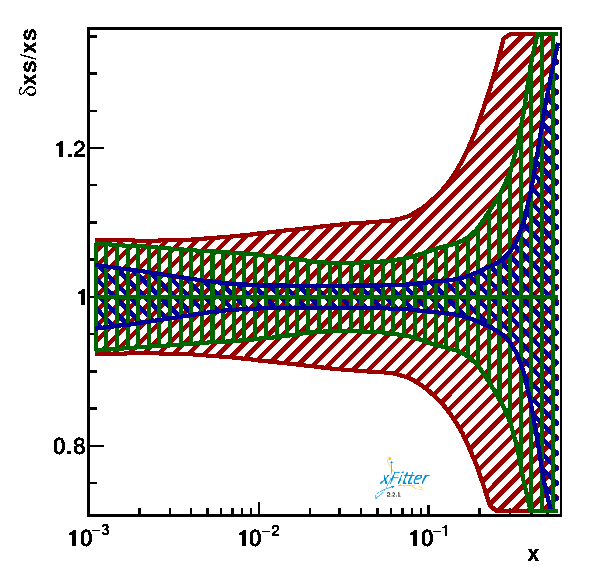
\includegraphics[width=0.32\textwidth]{plots/proton_fasernu2/FASERv2_vs_AdvSND/statOnly_AdvSND_q2_10000_pdf_s_ratio.pdf}\\
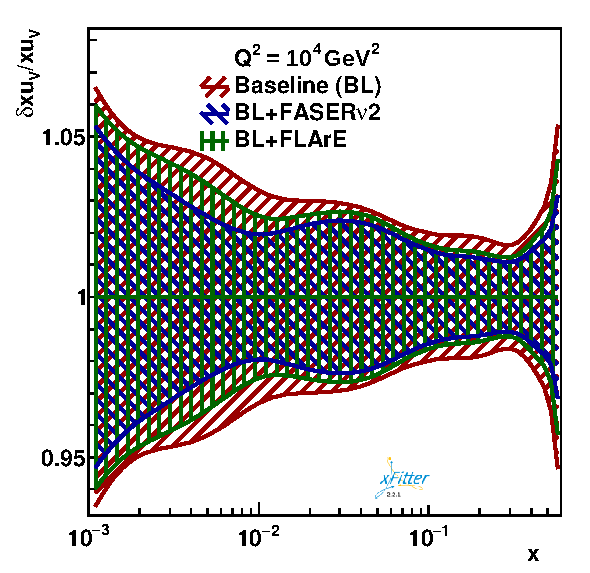
\includegraphics[width=0.32\textwidth]{plots/proton_fasernu2/FASERv2_vs_FLArE10/statOnly_FLArE10_q2_10000_pdf_uv_ratio.pdf}
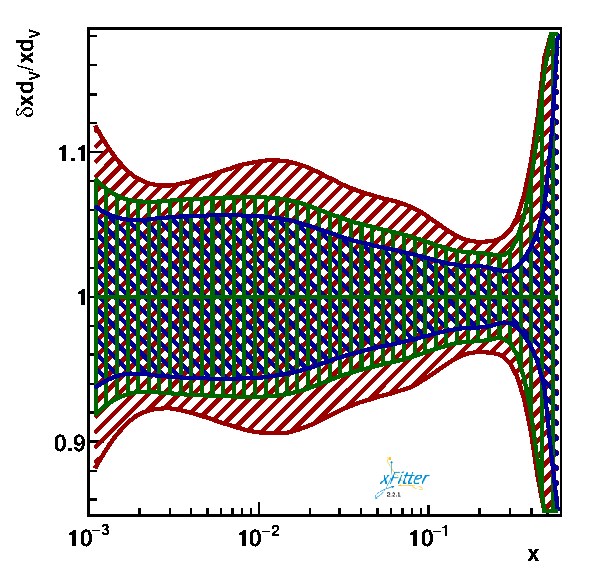
\includegraphics[width=0.32\textwidth]{plots/proton_fasernu2/FASERv2_vs_FLArE10/statOnly_FLArE10_q2_10000_pdf_dv_ratio.pdf}
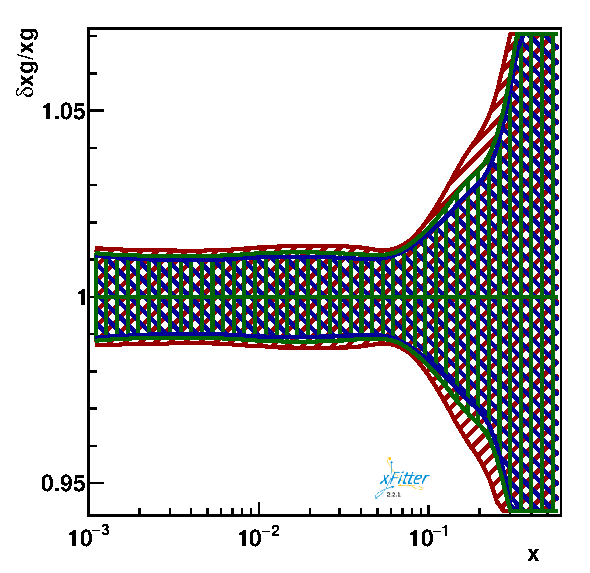
\includegraphics[width=0.32\textwidth]{plots/proton_fasernu2/FASERv2_vs_FLArE10/statOnly_FLArE10_q2_10000_pdf_g_ratio.pdf}\\
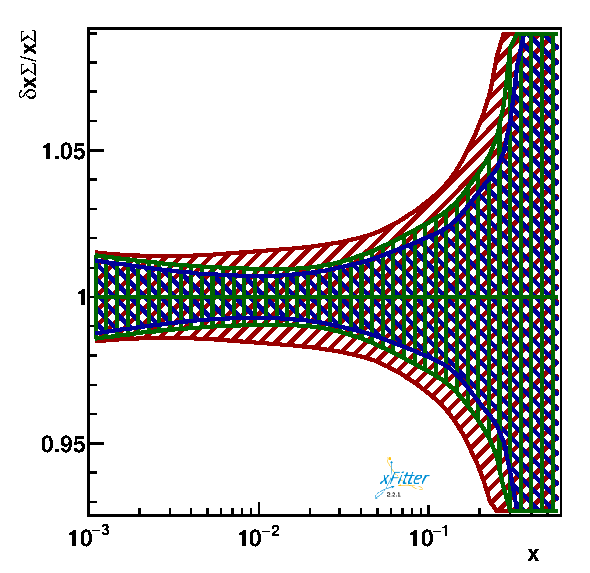
\includegraphics[width=0.32\textwidth]{plots/proton_fasernu2/FASERv2_vs_FLArE10/statOnly_FLArE10_q2_10000_pdf_Sea_ratio.pdf}
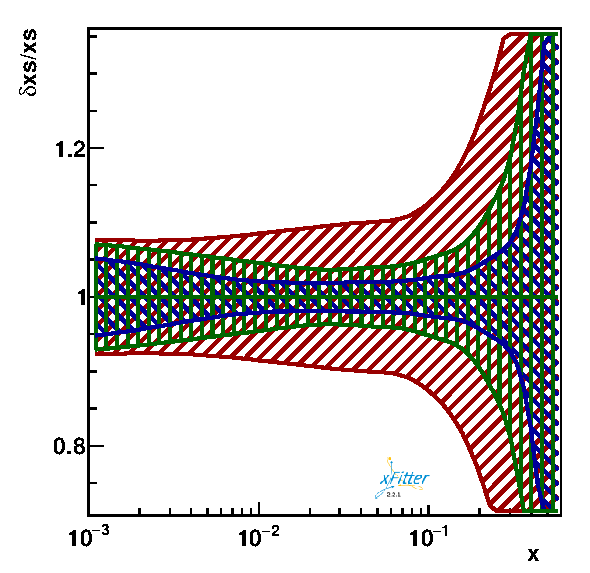
\includegraphics[width=0.32\textwidth]{plots/proton_fasernu2/FASERv2_vs_FLArE10/statOnly_FLArE10_q2_10000_pdf_s_ratio.pdf}
\caption{
  Same as Fig.~\ref{fig:FASERnu2_baseline} (statistical uncertainties only),
  comparing
  the projected PDF impact of FASER$\nu$2 with that of  AdvSND (top panels) and FLArE10 (bottom panels). 
}
\label{fig:FASERnu2_FLAre10}
\end{figure}
%%%%%%%%%%%%%%%%%%%%%%%%%%%%%%%%%%%%%%%%%%%%%%%%%%%%%%%%%%%%%%%%%%%%%%

From Fig.~\ref{fig:FASERnu2_FLAre10} one can see that the three
FPF experiments studied lead to a reduction of the  uncertainties in the quark PDFs.
%
By comparing their relative impact, we find that the constraints
achieved by FASER$\nu$2 are somewhat better than for the other two experiments,
as could have been expected by the larger event yields obtained in the former.
%
In the case of AdvSND, the  smaller sample of charm-tagged events is responsible for the reduction
in the constraints on strangeness.
%
Another consequence of the smaller event rates in AdvSND and FLArE10 as compared
to FASER$\nu$2 is the milder impact for the $x\lsim 10^{-2}$ region,
which can only be properly covered once the integrated statistics become large
enough,  as indicated by the differential bin-by-bin yields displayed in Fig.~\ref{fig:fasernu2_muon}.

We note here that Fig.~\ref{fig:FASERnu2_FLAre10} compares fits based on FPF pseudo-data
with only statistical uncertainties, and that a more refined comparison between the PDF reach of
the various FPF experiments requires accounting also for the systematic uncertainties, which ultimately become
one of the limiting factors.
%
Also, as mentioned above, cross-calibration between experiments should provide
valuable input to enhance the PDF sensitivity.

To conclude this discussion, applying the same procedure to FASER$\nu$ and SND@LHC structure
functions leaves the baseline PDF4LHC21 results unaffected, as demonstrated in App.~\ref{app:fasernu_runIII_impact},
showing that for the current generation of LHC neutrino detectors
it will be difficult to provide competitive constraints on the proton structure.

\paragraph{Combined impact of the FPF experiments.}
%
Finally, we have carried out a further PDF analysis including simultaneously the three FPF experiments
considered so far: FASER$\nu$2, AdvSND, and FLArE100.
%
Fig.~\ref{fig:FPF_combined} displays the combined impact of the FPF experiments when added
on top of the  PDF4LHC21 baseline by means of Hessian profiling, both in the statistics-only case and
when systematic and statistical uncertainties are added in quadrature.
%
Possible correlations between the individual experiments are neglected in this exercise, though they
will become important when interpreting the actual measurements.

%%%%%%%%%%%%%%%%%%%%%%%%%%%%%%%%%%%%%%%%%%%%%%%%%%%%%%%%%%%%%%%%%%%%%%%
\begin{figure}[t]
\centering
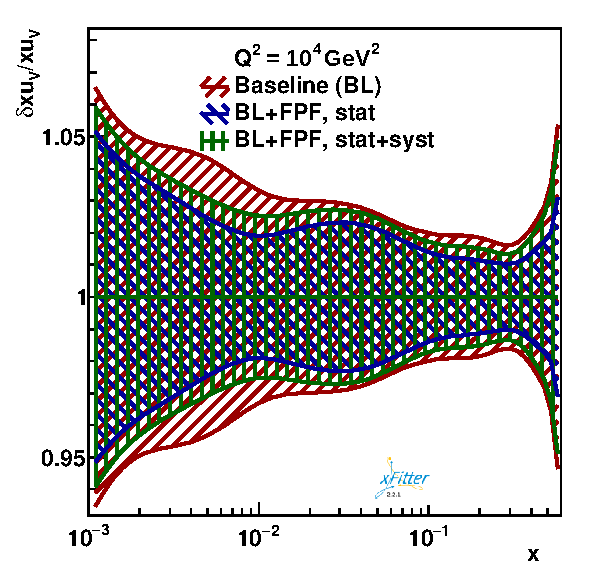
\includegraphics[width=0.32\textwidth]{plots/proton_fasernu2/FPF/fred05fcorr05_FPF_q2_10000_pdf_uv_ratio.pdf}
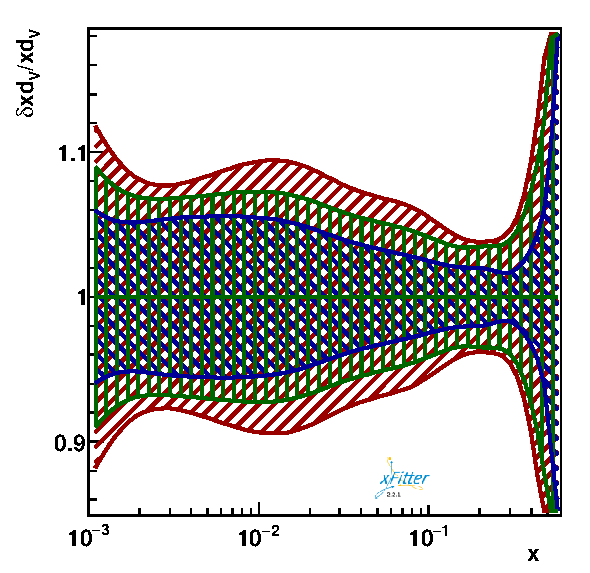
\includegraphics[width=0.32\textwidth]{plots/proton_fasernu2/FPF/fred05fcorr05_FPF_q2_10000_pdf_dv_ratio.pdf}
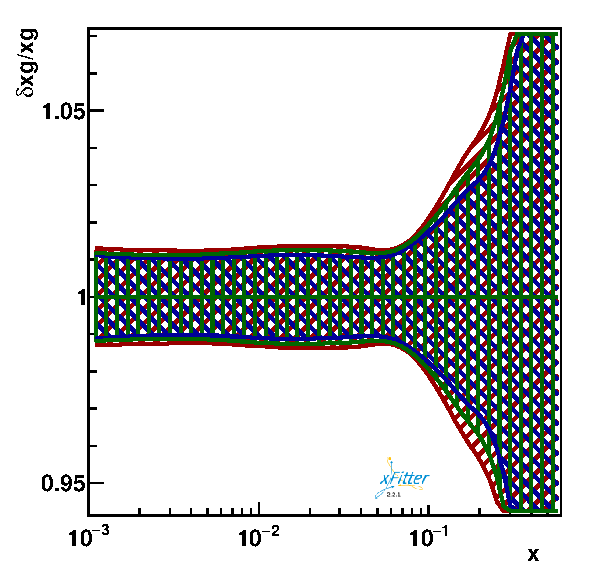
\includegraphics[width=0.32\textwidth]{plots/proton_fasernu2/FPF/fred05fcorr05_FPF_q2_10000_pdf_g_ratio.pdf}\\
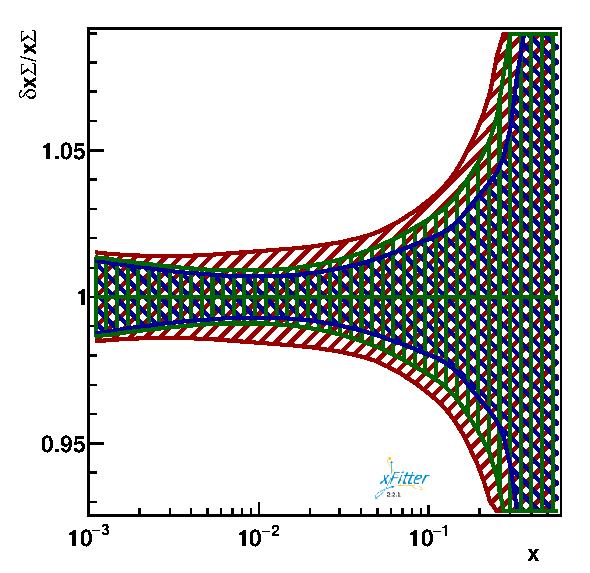
\includegraphics[width=0.32\textwidth]{plots/proton_fasernu2/FPF/fred05fcorr05_FPF_q2_10000_pdf_Sea_ratio.pdf}
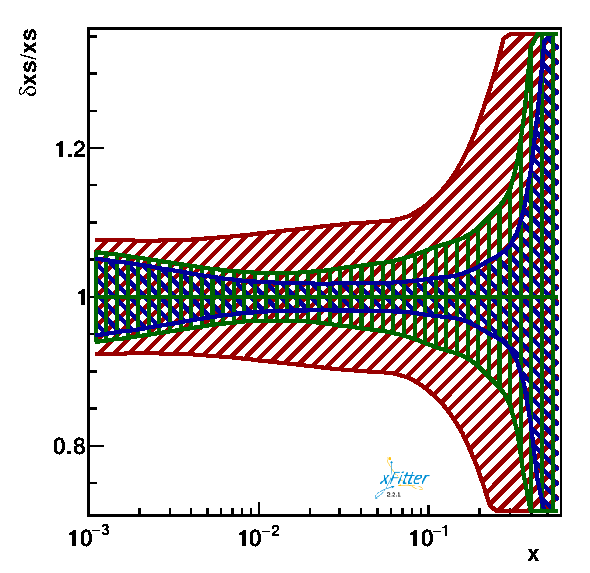
\includegraphics[width=0.32\textwidth]{plots/proton_fasernu2/FPF/fred05fcorr05_FPF_q2_10000_pdf_s_ratio.pdf}
\caption{
  Same as Fig.~\ref{fig:FASERnu2_baseline} now quantifying the
  projected PDF impact of the three FPF experiments added simultaneously to
  the analysis: FASER$\nu$2, AdvSND, and FLArE10. 
}
\label{fig:FPF_combined}
\end{figure}
%%%%%%%%%%%%%%%%%%%%%%%%%%%%%%%%%%%%%%%%%%%%%%%%%%%%%%%%%%%%%%%%%%%%%%%

The combined impact of the three FPF experiments on PDF4LHC21 shown in Fig.~\ref{fig:FPF_combined}
is only slightly improved as compared to the results of the FASER$\nu$2-only profiling
in Fig.~\ref{fig:FASERnu2_baseline}.
%
This shows that in this naive combination of experiments the one with the largest individual
sensitivity dominates, in this case FASER$\nu$2.
%
Again, this exercise is somewhat simplistic since within the real experiments the consistency (or lack thereof) between
individual measurements, which here is assumed by construction, provides useful information, and also
because the FPF experiments will cross-calibrate each other and cover somewhat different kinematic regions.

All in all, Fig.~\ref{fig:FPF_combined}, and in particular the statistics-only case, represents
a best-case scenario for the reduction of PDF uncertainties which can be expected from
the analysis of neutrino DIS structure function data at the FPF, in the assumption that PDF4LHC21 accurately represents
our current knowledge about the quark and gluon structure of the proton.

\subsection{Proton PDFs: impact on NNPDF4.0}
\label{sec:nnpdf40}

As discussed in Sect.~\ref{subsec:pdf_impact_assessment}, the PDF sensitivity
studies of the FPF neutrino data based on the {\sc\small xFitter} profiling
of PDF4LHC21 are complemented by those based on their direct inclusion
in the NNPDF4.0 global analysis.
%
Here we present results for the impact of the combined FPF neutrino
measurements on NNPDF4.0, namely the analogous study of that shown
in Fig.~\ref{fig:FPF_combined} in the case of PDF4LHC21.
%
We emphasize that we have produced results for the variations studied in
Sect.~\ref{sec:pdf4lhc21} also with the NNPDF fitting methodology.
%
Given that the qualitative obtained with the NNPDF fits
are compatible with those obtained with {\sc\small xFitter}, it is not necessary to duplicate them here,
and hence we only show results for the impact of the combined FPF pseudo-data.

Fig.~\ref{fig:NNPDF40_baseline} displays the
same results as Fig.~\ref{fig:FPF_combined} now in the case of the
fits obtained with the NNPDF4.0 fitting methodology.
%
The baseline NNPDF4.0 NNLO analysis is compared
with the results of the fits which include the combined FPF dataset,
in both the statistics-only scenario and for the case
where systematic uncertainties are also accounted for.
%
As in the PDF4LHC21 analysis, the bands indicate the one-sigma PDF uncertainties.
%
Note that we also show results for the charm PDF (bottom right panel), which
in the NNPDF4.0 fit is also determined directly from the data entering
the fit~\cite{Ball:2016neh}.
%
In this way, we can determine the possible constraints that neutrino
DIS measurements at the LHC may impose on the intrinsic charm
content of the proton~\cite{Ball:2022qks}.

 %%%%%%%%%%%%%%%%%%%%%%%%%%%%%%%%%%%%%%%%%%%%%%%%%%%%%%%%%%%%%%%%%%%%%%%%
\begin{figure}[t]
\centering
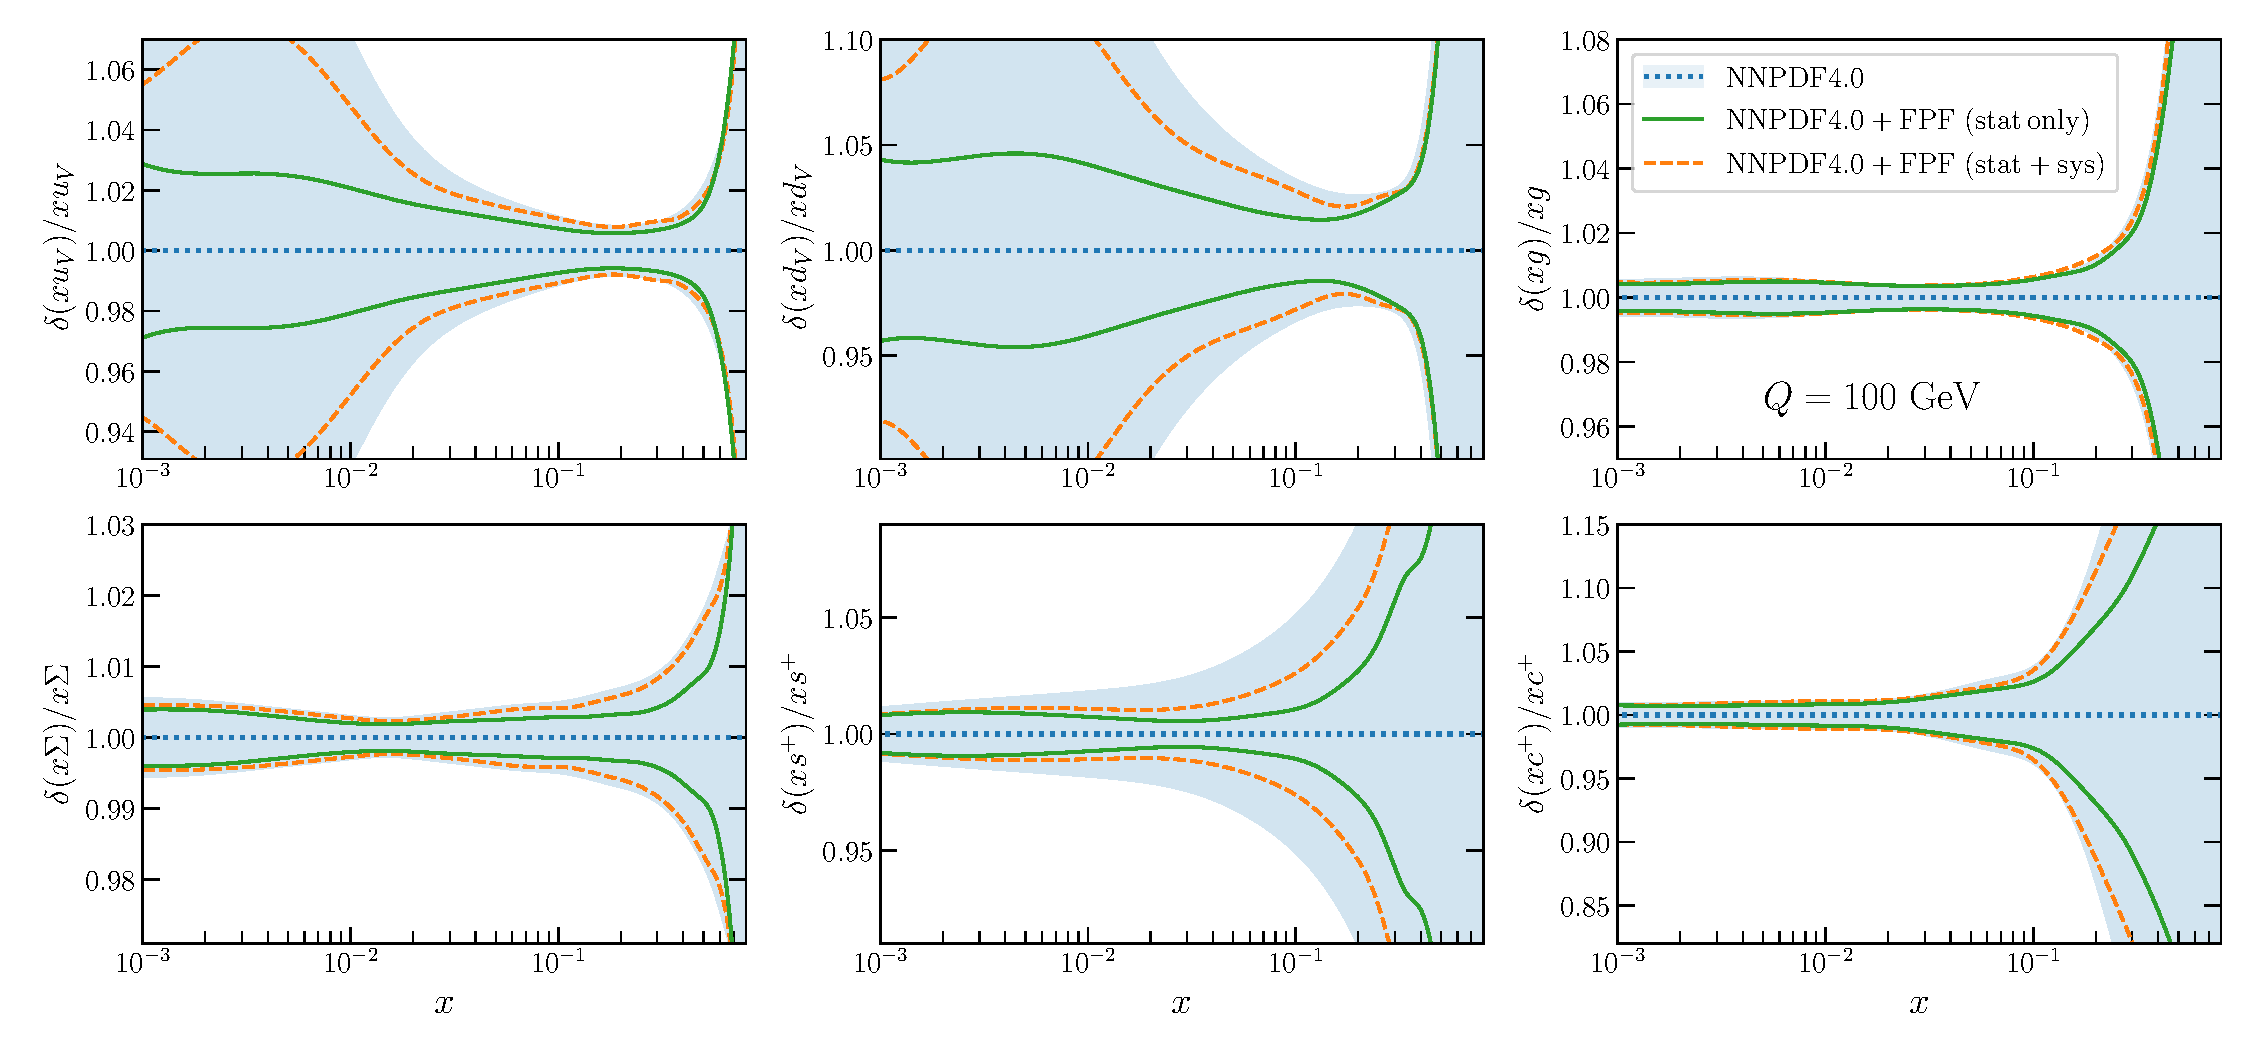
\includegraphics[width=0.99\textwidth]{plots/NNPDF40-FPFall-q100gev.pdf}
\caption{
  Same as Fig.~\ref{fig:FPF_combined} for the results obtained
  using the NNPDF4.0 fitting methodology.
  %
  The baseline NNPDF4.0 NNLO analysis is compared
  with the results of the fits which include the combined FPF dataset
  in both the statistics-only scenario and for the case
  where systematic uncertainties are also accounted for.
  %
  As in the PDF4LHC21 case, the bands indicate the one-sigma PDF uncertainties.
  %
  We now also show results for the charm PDF (bottom right panel), which
  in the NNPDF4.0 fit is also determined directly from the data entering the fit.
%
}
\label{fig:NNPDF40_baseline}
\end{figure}
%%%%%%%%%%%%%%%%%%%%%%%%%%%%%%%%%%%%%%%%%%%%%%%%%%%%%%%%%%%%%%%%%%%%%%%%

From  Fig.~\ref{fig:NNPDF40_baseline} one finds that
the impact on the PDFs found by direct inclusion of the FPF structure
functions on the NNPDF4.0 fit is qualitatively consistent with
that found in the the Hessian profiling of PDF4LHC21.
%
In particular, the constraints are more significant for the up and down
quark valence PDFs as well as for the total strangeness.
%
As was the case with the PDF4LHC21 baseline, the uncertainty reduction
for the strangeness PDF is particularly
striking.
%
Also consistently with the results of Sect.~\ref{sec:pdf4lhc21}, the gluon
PDF is unchanged, and the impact on the total quark PDF
is restricted to the large-$x$ region.
%
While one can also identify differences related to analysis choices
such as the PDF parametrisation and the method used to assess the PDF
error reduction (for example, concerning the small-$x$ behaviour of $xu_V$ and $xd_V$)
we conclude that by and large the projected impact of the FPF structure function
measurements is independent of the specific fitting methodology adopted.

 %%%%%%%%%%%%%%%%%%%%%%%%%%%%%%%%%%%%%%%%%%%%%%%%%%%%%%%%%%%%%%%%%%%%%%%%
\begin{figure}[t]
\centering
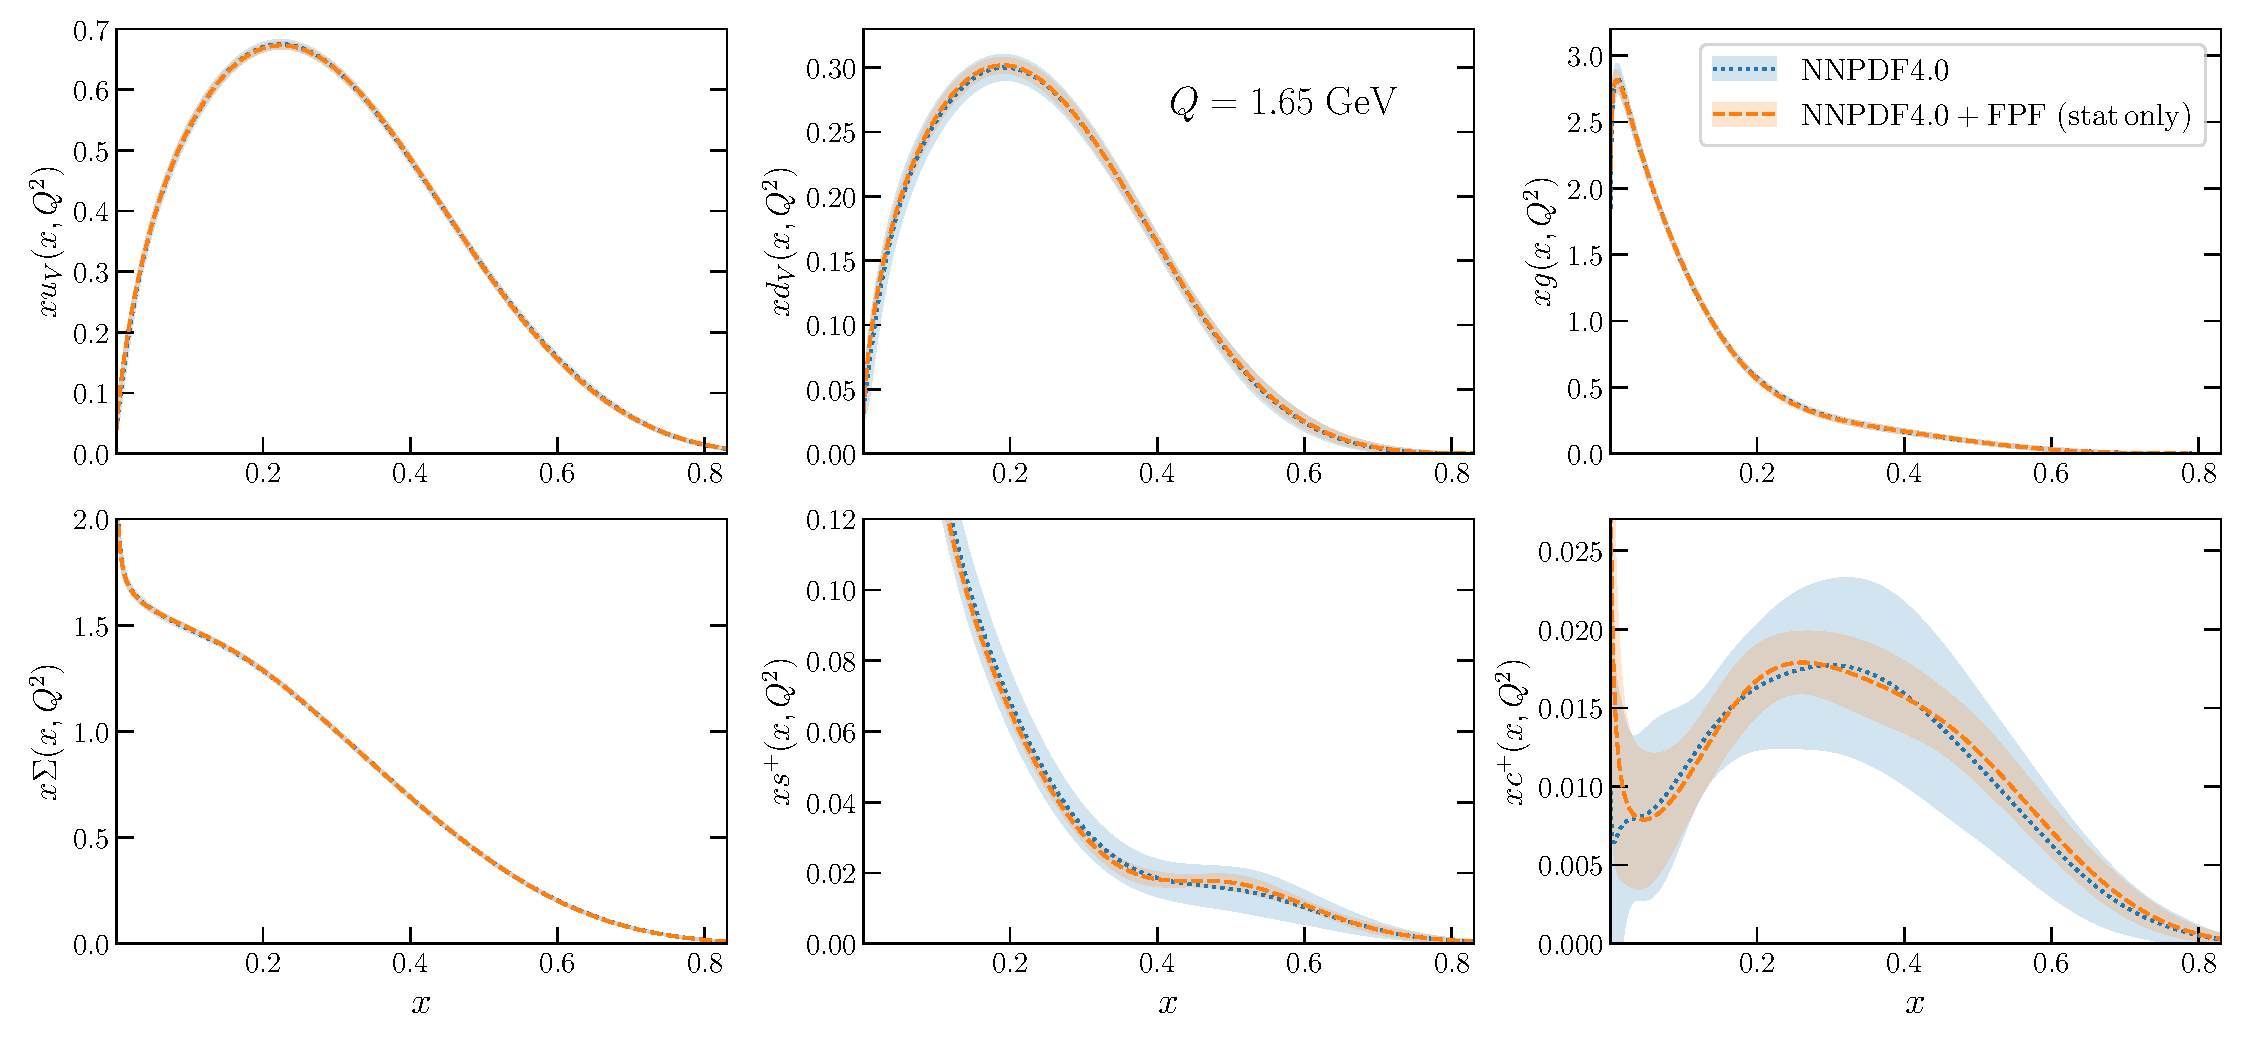
\includegraphics[width=0.99\textwidth]{plots/NNPDF40-FPFall-q1p65gev-abs.pdf}
\caption{
  Same as Fig.~\ref{fig:NNPDF40_baseline} now for the absolute PDFs
  at the initial parametrisation scale, $Q=1.65$ GeV, focusing
  on the large-$x$ region.
%
}
\label{fig:NNPDF40_lowQ_abs}
\end{figure}
%%%%%%%%%%%%%%%%%%%%%%%%%%%%%%%%%%%%%%%%%%%%%%%%%%%%%%%%%%%%%%%%%%%%%%%%

As indicated by Fig.~\ref{fig:NNPDF40_baseline}, the FPF data is also expected
to reduce the uncertainties associated to the fitted charm PDF in the region $x\simeq 0.2$
dominated by the non-perturbative component.
%
In order to highlight this impact on the large-$x$ region of the PDFs,
Fig.~\ref{fig:NNPDF40_lowQ_abs} presents the same comparison as
in  Fig.~\ref{fig:NNPDF40_baseline} now for the absolute PDFs
at the initial parametrisation scale, $Q=1.65$ GeV, using a linear scale, for the statistics-only
scenario.
%
One can observe the improved constraints on the charm PDF in the large-$x$ region,
further confirming previous studies~\cite{Anchordoqui:2021ghd,Feng:2022inv} that indicate the
sensitivity of the FPF to the intrinsic charm content of the proton.
%
This comparison also illustrates the excellent constraining power on the proton
strangeness enabled by the FPF charm-tagged structure function data.

%-----------------------------------------------------------------------
\begin{table}[!t]
  \centering
  \footnotesize
  \renewcommand{\arraystretch}{1.30}
  \begin{tabularx}{\textwidth}{X|l|c|c|c}
  \toprule
  & \multirow{3}{*}{Dataset}
  & \multicolumn{3}{c}{\bf NNPDF4.0 NNLO} \\
  &
  & \multirow{2}{*}{Baseline}
  & \multicolumn{2}{c}{with combined FPF data}  \\
  &
  &
  & Statistical-only  & Statistical + systematics  \\
  \midrule
  $\chi^2$ &  \multirow{4}{*}{Global}  & 1.170 &  1.161  & 1.145  \\
  $\la E_{\rm tr}\ra_{\rm rep}$
  &  &  2.256  &  2.242   & 2.215   \\
  $\la E_{\rm val}\ra_{\rm rep}$
  & & 2.360    &   2.332  & 2.311  \\
  $\la \chi^2\ra_{\rm rep}$
  & &   1.194   &    1.187    & 1.169  \\
  \midrule
  \multirow{8}{*}{$\chi^2$}
  & DIS neutral-current                     &  1.220    &  1.230    &   1.220   \\
  & DIS charged-current                     &   0.904  &   0.942    &  0.913    \\
  & Drell--Yan (inclusive and one-jet) &  1.76   &   1.830    &   1.830   \\
  & Top-quark pair production               &  1.230   &   1.220    &  1.250    \\
  & Single-top production                   &  0.362   &   0.364    &   0.361   \\
  & Inclusive jet production                &  0.957   &  0.963     &   0.942   \\
  & Dijet production                        &  2.030    &    2.010   &   2.010   \\
  & Direct photon production                 &  0.740  &   0.729    &    0.744  \\
  & FPF (total)                 &  -  &       &      \\
  \bottomrule
\end{tabularx}
\vspace{0.2cm}
\caption{\small Statistical estimators for the NNPDF4.0 NNLO
  baseline fit, compared to the variants including
  the combined FPF dataset shown in Figs.~\ref{fig:NNPDF40_baseline}
  and~\ref{fig:NNPDF40_lowQ_abs}.
  %
  From top to bottom: total $\chi^2$, average
  over replicas of the training and validation figures of merit
  $\la E_{\rm tr}\ra_{\rm rep}$ and $\la E_{\rm val}\ra_{\rm rep}$,
  average $\chi^2$ over replicas $\la \chi^2\ra_{\rm rep}$,
  $\chi^2$ for datasets grouped by process.
  %
  The last row displays the $\chi^2$ obtained for the combined FPF dataset.
  \label{tab:chi2_nnpdf40_baseline}
}
\end{table}
%--------------------------------------------------------------------------

The statistical estimators for the NNPDF4.0 NNLO
baseline fit, compared to the variants including
the combined FPF dataset shown in Figs.~\ref{fig:NNPDF40_baseline}
and~\ref{fig:NNPDF40_lowQ_abs}, are reported in Table~\ref{tab:chi2_nnpdf40_baseline}.
%
From top to bottom we indicate the total $\chi^2$, average
over replicas of the training and validation figures of merit
$\la E_{\rm tr}\ra_{\rm rep}$ and $\la E_{\rm val}\ra_{\rm rep}$,
average $\chi^2$ over replicas $\la \chi^2\ra_{\rm rep}$,
$\chi^2$ for datasets grouped by process.
%
Note that the last row displays the $\chi^2$ obtained for the combined FPF dataset.
%
For the latter, one finds that as expected $\chi^2 \sim 1$, given that the FPF pseudo-data
is produced by construction to be fully compatible with the NNPDF4.0 baseline.
%
For the same reason, the description of all other experiments entering
the NNPDF4.0 global fit is not distorted by the inclusion of the FPF data.
%
In particular, the $\chi^2$ of the available (non-FPF) DIS neutral-current and charged-current
datasets changes from 1.220 and 0.904 in NNPDF4.0 to 1.220 and 0.913 in the fit
with FPF pseudo-data.
%
A moderate increase is found to the $\chi^2$ of Drell-Yan processes, from 1.76 to 1.83, possibly
because of the enhanced weight that DIS data carries in this fit variant.

Fig.~\ref{fig:nnpdf40_fpf_lumis} displays a comparison of the PDF luminosities at $\sqrt{s}=14$ TeV
as a function of the final-state invariant mass $m_X$ between
the baseline NNPDF4.0 NNLO determination and its variant which includes
the combined FPF pseudo-data from the FASER$\nu$2, FLArE100, and AdvSND experiments,
see Figs.~\ref{fig:NNPDF40_baseline} or the corresponding PDF comparison.
%
%
  Results are shown normalised to the central value of the NNPDF4.0 baseline.
  %
  Specifically, we show the gluon-gluon, quark-antiquark, and
  quark-quark luminosities.
  %
These luminosities are useful to interpret the phenomenological studies with the FPF-improved
PDFs for the HL-LHC that will be presented in Sect.~\ref{sec:pheno}.

%%%%%%%%%%%%%%%%%%%%%%%%%%%%%%%%%%%%%%%%%%%%%%%%%%%%%%%%%%%%%%%%%%%%%%%%
\begin{figure}[t]
\centering
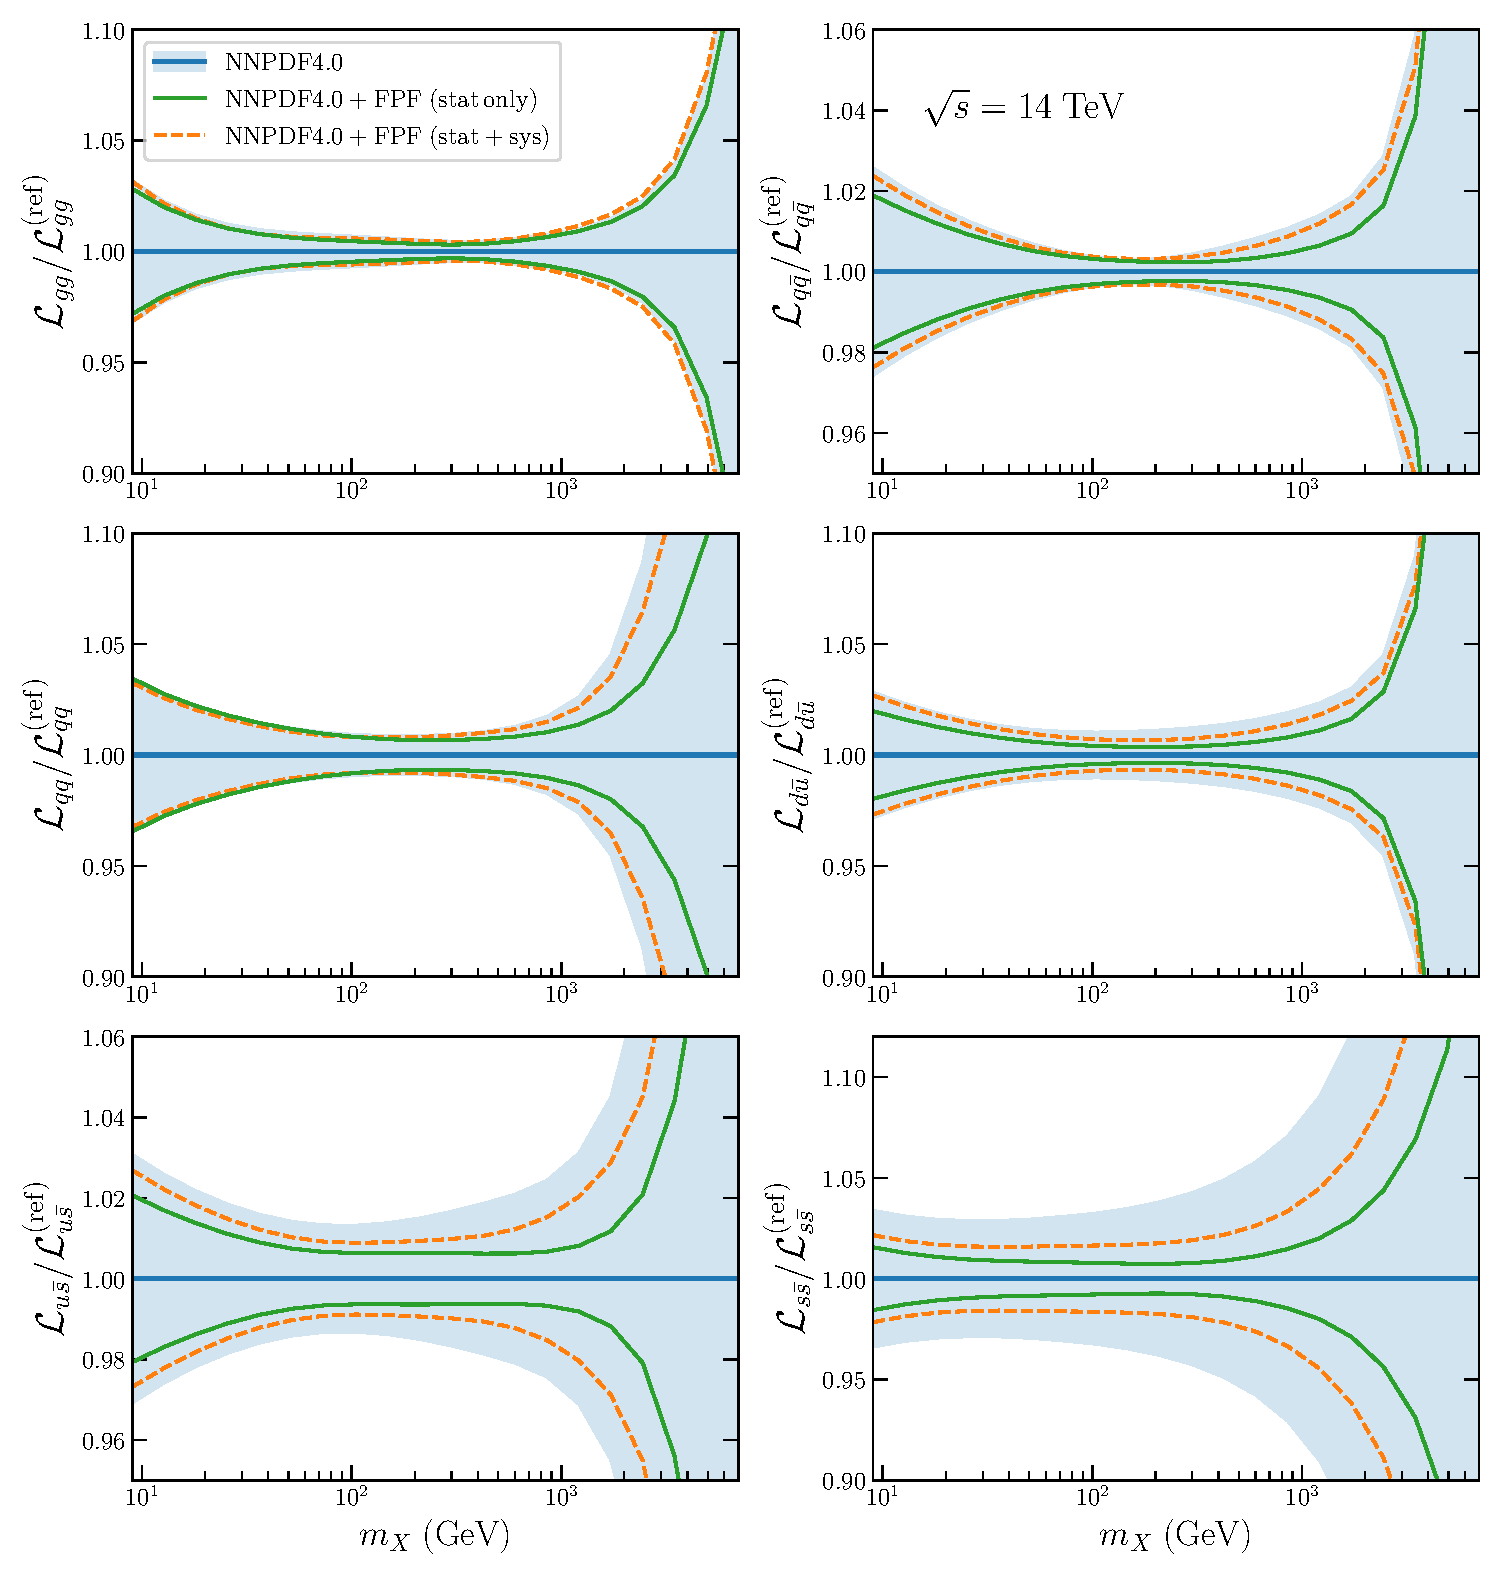
\includegraphics[width=0.99\textwidth]{plots/lumi-FPFall.pdf}
\caption{Comparison of the PDF luminosities at $\sqrt{s}=14$ TeV
  as a function of the final-state invariant mass $m_X$ between
  the baseline NNPDF4.0 NNLO determination and its variants which include
  the full set of FPF pseudo-data, see Figs.~\ref{fig:NNPDF40_baseline}
  for the corresponding PDF comparison.
  %
  Results are shown normalised to the central value of the NNPDF4.0 baseline.
  %
  From left to right we show the gluon-gluon, quark-antiquark, and
  quark-quark luminosities.
%
}
\label{fig:nnpdf40_fpf_lumis}
\end{figure}
%%%%%%%%%%%%%%%%%%%%%%%%%%%%%%%%%%%%%%%%%%%%%%%%%%%%%%%%%%%%%%%%%%%%%%%%

The reduction of PDF uncertainties found in  Figs.~\ref{fig:NNPDF40_baseline}
and~\ref{fig:NNPDF40_lowQ_abs} is also visible
for the partonic luminosities, specially on the scenario where only statistical
uncertainties in the FPF pseudo-data are considered.
%
The improvement quark-antiquark luminosities at $Q\sim 100$ GeV
benefits theoretical predictions for $W$ and $Z$ production at the LHC.
%
It is also worth noting the PDF error reduction for the quark-quark luminosity at high invariant masses,
which will feed into searches for new heavy particles at the TeV scale driven by quark-initiated scattering.

\subsection{Nuclear PDFs: impact on EPPS21}
\label{sec:nuclearPDFs}

The studies presented in Sects.~\ref{sec:pdf4lhc21} (for PDF4LHC21)
and~\ref{sec:nnpdf40} (for NNPDF4.0) treated, from the point of view
of PDF constraints, the neutrino scattering target
as composed by isoscalar free-nucleons.
%
They hence neglected both nuclear modifications
and non-isoscalar effects.
%
We now revisit these analyses but accounting for the fact that the target materials
in the FASER$\nu$2 and AdvSND experiments is tungsten, with $A=184$.
%
In this exercise we do not include the FLArE structure function data,
corresponding to a different target material (liquid argon, with $A=40$), although
in an actual nuclear PDF fit all FPF datasets would be included simultaneously.
%
Nuclear modifications associated to a tungsten target, when compared
to a free isoscalar nucleon, are not necessarily small, and  will affect the event rate predictions for
the FPF experiments.
%
This fact also implies that  measurements of differential neutrino cross-sections
on heavy nuclear targets provide direct constraints on these nuclear modifications
without relying on assumptions on their $A$ dependence.

We quantify the impact of the FPF structure function measurements
on the nuclear PDFs of tungsten by applying the same Hessian profiling
of Sects.~\ref{sec:pdf4lhc21} to EPPS1, a global determination of nuclear PDFs
that accounts for the constraints of existing datasets involving nuclei as target or projectiles.
%
We note that EPPS21 already includes information from neutrino DIS on nuclear targets
from the CHORUS and NuTeV experiments.
%
EPPS21 is generally in good agreement with other recent nPDF fits such as nNNPDF3.0~\cite{AbdulKhalek:2022fyi}
and nCTEQ15HQ~\cite{Duwentaster:2022kpv}.
%
The application of profiling to EPPS21 follows the same strategy as that
for PDF4LHC21, with the caveat that its Hessian error sets also include the contribution
from the uncertainties  associated to their reference proton PDF set, in this case CT18.
%
Given that the measured event rates depend on both the proton PDFs and the nuclear modifications,
when profiling EPPS21 we also account for the Hessian sets associated to the CT18 proton
PDF dependence.
%
Also relevant for the subsequent discussion, EPPS21 adopts a tolerance
factor of $T^2 = 20$ when defining their  68\%  confidence level uncertainties,
to be contrasted with  $T^2 = 10$ used in PDF4LHC21.


 
%%%%%%%%%%%%%%%%%%%%%%%%%%%%%%%%%%%%%%%%%%%%%%%%%%%%%%%%%%%%%%%%%%%%%%%%
\begin{figure}[t]
\centering
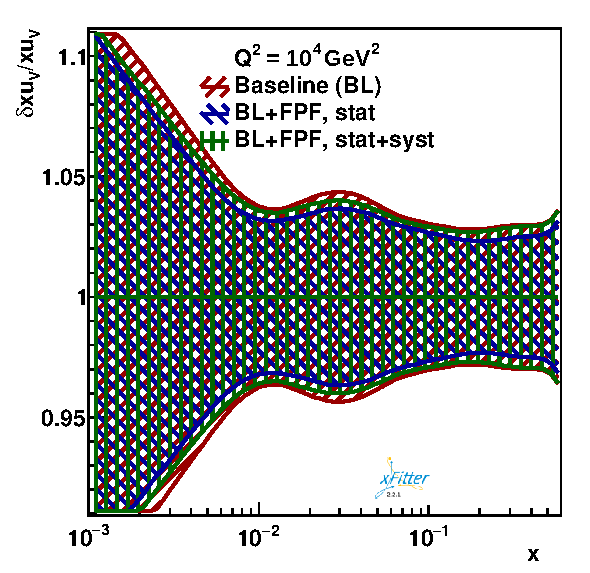
\includegraphics[width=0.32\textwidth]{plots/nuclear_fasernu2/FPF/fred05fcorr05_FPF_q2_10000_pdf_uv_ratio.pdf}
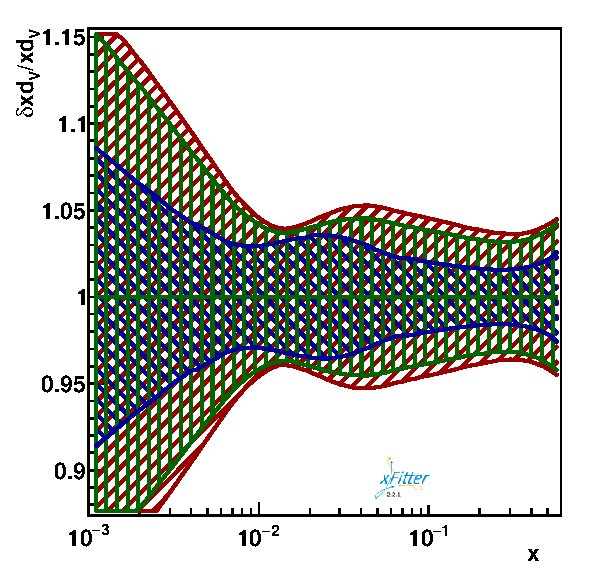
\includegraphics[width=0.32\textwidth]{plots/nuclear_fasernu2/FPF/fred05fcorr05_FPF_q2_10000_pdf_dv_ratio.pdf}
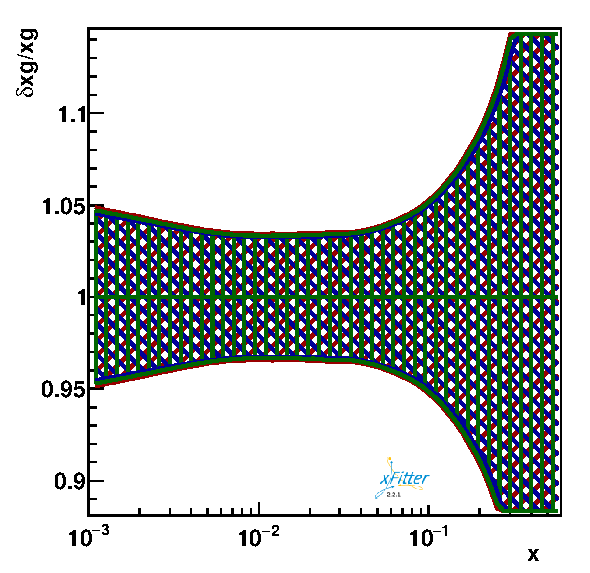
\includegraphics[width=0.32\textwidth]{plots/nuclear_fasernu2/FPF/fred05fcorr05_FPF_q2_10000_pdf_g_ratio.pdf}\\
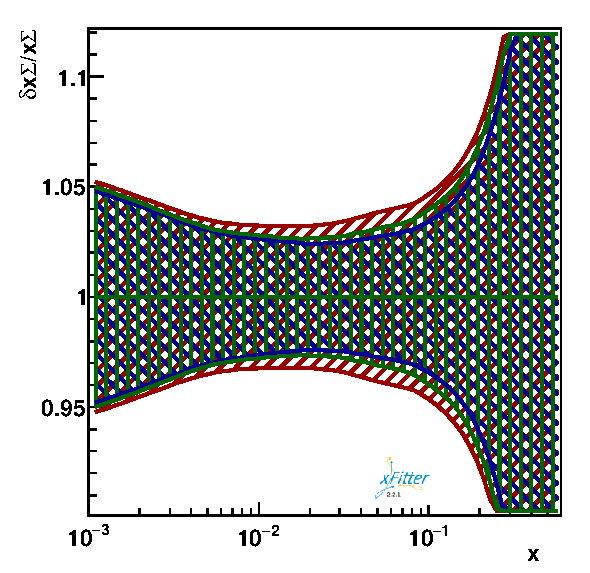
\includegraphics[width=0.32\textwidth]{plots/nuclear_fasernu2/FPF/fred05fcorr05_FPF_q2_10000_pdf_Sea_ratio.pdf}
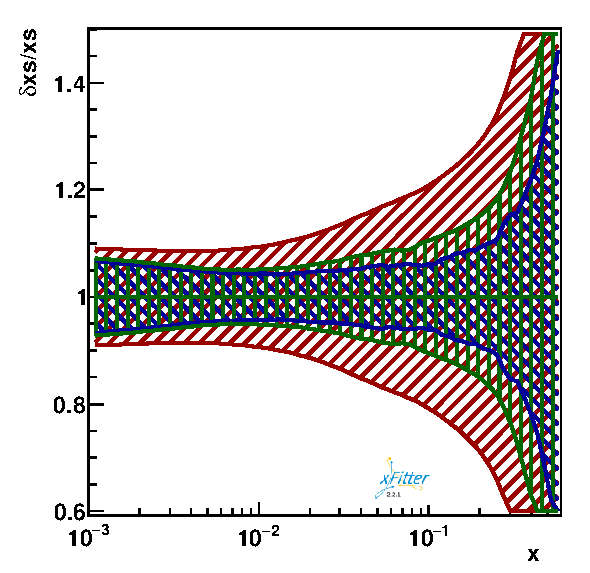
\includegraphics[width=0.32\textwidth]{plots/nuclear_fasernu2/FPF/fred05fcorr05_FPF_q2_10000_pdf_s_ratio.pdf}
\caption{Same as Fig.~\ref{fig:FPF_combined} now corresponding to the Hessian
 profiling of EPPS21 for a tungsten nucleus.
}
\label{fig:profiling_FPF_nuclear}
\end{figure}
%%%%%%%%%%%%%%%%%%%%%%%%%%%%%%%%%%%%%%%%%%%%%%%%%%%%%%%%%%%%%%%%%%%%%%%%

Fig.~\ref{fig:profiling_FPF_nuclear} displays a similar comparison as that of
 Fig.~\ref{fig:FPF_combined}, now corresponding to the Hessian
 profiling of EPPS21 for a tungsten nucleus.
 %
 The FPF dataset is in this case composed by FASER$\nu$2 and AdvSND, given that FLArE
 adopts a different target material.
 %
 Also in this case of nuclear PDFs one finds that the impact of FPF structure function measurements
 is most important for the strange PDF, and to a lesser extent for the up and down
 valence quark PDFs.
 %
 For the latter, the projected impact of FPF measurements appears to be somewhat milder
 as in the case of PDF4LHC21, specially once systematic uncertainties are taken into account.

 While the main qualitative features of the nPDF profiling are consistent with the free-proton
 case, one reason explaining the observed differences is the choice of a larger tolerance factor $T$ in EPPS21
 as compared to PDF4HC21, which effectively reduces the impact of new data.
 %
 Another reason is the more restrictive functional form adopted in EPPS21 as compared
 to the PDF sets entering PDF4LHC21, a consequence of the smaller dataset available
 for hard scattering on nuclear targets.
 %
 Given that these  functional forms are fixed when applying Hessian profiling,
 assessing the impact on a nuclear PDFs by a direct refit, as was done for NNPDF4.0,
 may provide a more  robust estimate of the impact of FPF structure function data
 on nuclear PDFs.
 %
 Additional results for the Hessian profiling of EPPS21 are presented in App.~\ref{app:nPDF_impact_appendix}.

\section{Implications for HL-LHC processes}
\label{sec:pheno}

The reduction of PDF uncertainties enabled by the neutrino DIS measurements
at the FPF presented in Sect.~\ref{sec:protonPDFs}
makes possible more precise theoretical predictions for key processes at the
HL-LHC.
%
Here we present an initial study of the phenomenological implications
of PDFs enhanced with LHC neutrino data.
%
We adopt the same settings as in the LHC phenomenology analysis presented
in the PDF4LHC21 combination paper~\cite{PDF4LHCWorkingGroup:2022cjn} and provide predictions
both for inclusive fiducial cross-sections and for differential distributions.
%
Specifically, we present results for 
single and double gauge boson production, inclusive top quark pair production,
and Higgs production in gluon
fusion and in association with a vector boson.
%
We evaluate these cross-sections using NLO matrix elements
which include  both in the
QCD and electroweak corrections using
{\sc\small mg5\_amc@nlo}~\cite{Frederix:2018nkq}
interfaced to {\sc\small PineAPPL}~\cite{Carrazza:2020gss}.
%
For all processes, realistic selection and acceptance cuts on the final state particles
have been applied, and PDF uncertainty bands correspond to 90\% CL
uncertainties.
%
No further theory uncertainties are considered in this
analysis.

Fig.~\ref{fig:NNPDF40_pheno_integrated} displays
fiducial cross-section for representative LHC processes at $\sqrt{s}=14$ TeV
evaluated with NNPDF4.0 NNLO, compared with the fits including the FPF structure function projections.
%
For the latter, we display the variants based only on statistical uncertainties and that
which includes also systematic errors.
%
The central values are set to be the same as in the original NNPDF4.0 calculation in all cases.
%
See~\cite{NNPDF:2021njg} for the calculational settings.
%
From top to bottom, we show inclusive Drell-Yan production ($Z, W^+, W^-$), Higgs production
in vector-boson fusion, Higgs associated
production, and diboson production ($W^+W^-$, $W^+Z$, $W^-Z$).
%
We focus on processes dominated by quark-quark and quark-antiquark scattering, given
that the FPF structure functions would not have any impact on gluon-initiated
processes such as top quark pair production or Higgs production in gluon fusion.
%
The corresponding comparison at the level of differential distributions
are shown in Fig.~\ref{fig:NNPDF40_pheno_differential}.
%
As done for the fiducial cross-sections of Fig.~\ref{fig:NNPDF40_pheno_integrated},
we only indicate the relative PDF uncertainty in each fit, with central values
assumed to be the same by construction.


%%%%%%%%%%%%%%%%%%%%%%%%%%%%%%%%%%%%%%%%%%%%%%%%%%%%%%%%%%%%%%%%%%%%%%%%
\begin{figure}[t]
\centering
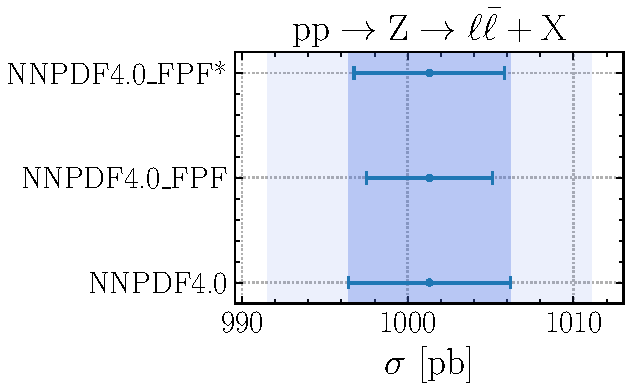
\includegraphics[width=0.32\textwidth]{plots/LHCpheno/NNPDF_DY_14TEV_40_PHENO-integrated.pdf}
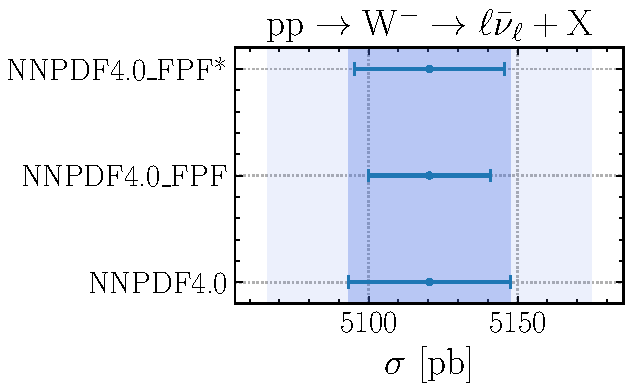
\includegraphics[width=0.32\textwidth]{plots/LHCpheno/NNPDF_WM_14TEV_40_PHENO-integrated.pdf}
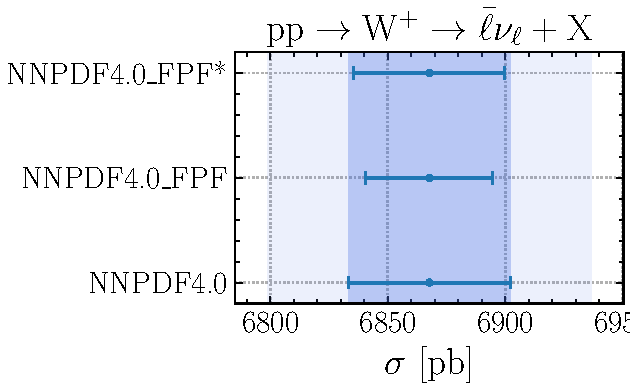
\includegraphics[width=0.32\textwidth]{plots/LHCpheno/NNPDF_WP_14TEV_40_PHENO-integrated.pdf}
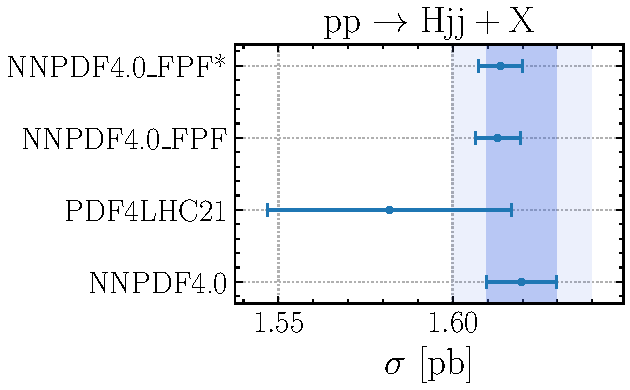
\includegraphics[width=0.32\textwidth]{plots/LHCpheno/NNPDF_HVBF_14TEV_40_PHENO-integrated.pdf}
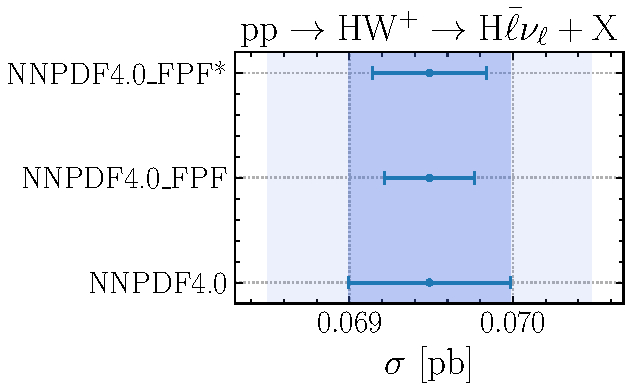
\includegraphics[width=0.32\textwidth]{plots/LHCpheno/NNPDF_HWP_14TEV_40_PHENO-integrated.pdf}
\includegraphics[width=0.32\textwidth]{plots/LHCpheno/NNPDF_HWM_14TEV_40_PHENO-integrated.pdf}
\includegraphics[width=0.32\textwidth]{plots/LHCpheno/NNPDF_WPWM_14TEV_40_PHENO-integrated.pdf}
\includegraphics[width=0.32\textwidth]{plots/LHCpheno/NNPDF_WPZ_14TEV_40_PHENO-integrated.pdf}
\includegraphics[width=0.32\textwidth]{plots/LHCpheno/NNPDF_WMZ_14TEV_40_PHENO-integrated.pdf}
\caption{Fiducial cross-sections for representative LHC processes at $\sqrt{s}=14$ TeV
evaluated with NNPDF4.0 NNLO, compared with the fits including the FPF structure function projections.
%
For the NNPDF4.0 baseline
prediction, the dark (light) bands indicate the 68\% (95\%) CL uncertainties.
%
The fit labelled as ``\_FPF'' is the one  based on statistical uncertainties,
while that labelled as ``\_FPF$^*$'' also includes systematic errors.
%
The central values are set to be the same as in the original NNPDF4.0 calculation in all cases.
%
See~\cite{NNPDF:2021njg,PDF4LHCWorkingGroup:2022cjn} for the calculational settings.
%
From top to bottom, we show inclusive Drell-Yan production ($Z, W^+, W^-$), Higgs production
in vector-boson fusion, Higgs associated
production, and diboson production ($W^+W^-$, $W^+Z$, $W^-Z$).
%
}
\label{fig:NNPDF40_pheno_integrated}
\end{figure}
%%%%%%%%%%%%%%%%%%%%%%%%%%%%%%%%%%%%%%%%%%%%%%%%%%%%%%%%%%%%%%%%%%%%%%%%


%%%%%%%%%%%%%%%%%%%%%%%%%%%%%%%%%%%%%%%%%%%%%%%%%%%%%%%%%%%%%%%%%%%%%%%%
\begin{figure}[htbp]
\centering
\includegraphics[width=0.49\textwidth]{plots/LHCpheno/NNPDF_DY_14TEV_40_PHENO-global.pdf}
\includegraphics[width=0.49\textwidth]{plots/LHCpheno/NNPDF_WM_14TEV_40_PHENO-global.pdf}
\includegraphics[width=0.49\textwidth]{plots/LHCpheno/NNPDF_WP_14TEV_40_PHENO-global.pdf}
\includegraphics[width=0.49\textwidth]{plots/LHCpheno/NNPDF_HVBF_14TEV_40_PHENO-global.pdf}
\includegraphics[width=0.49\textwidth]{plots/LHCpheno/NNPDF_HWP_14TEV_40_PHENO-global.pdf}
\includegraphics[width=0.49\textwidth]{plots/LHCpheno/NNPDF_HWM_14TEV_40_PHENO-global.pdf}
\includegraphics[width=0.49\textwidth]{plots/LHCpheno/NNPDF_WPWM_14TEV_40_PHENO-global.pdf}
\includegraphics[width=0.49\textwidth]{plots/LHCpheno/NNPDF_WPZ_14TEV_40_PHENO-global.pdf}
\includegraphics[width=0.49\textwidth]{plots/LHCpheno/NNPDF_WMZ_14TEV_40_PHENO-global.pdf}
\caption{Same as Fig.~\ref{fig:NNPDF40_pheno_integrated}
for the corresponding differential distributions.
%
}
\label{fig:NNPDF40_pheno_differential}
\end{figure}
%%%%%%%%%%%%%%%%%%%%%%%%%%%%%%%%%%%%%%%%%%%%%%%%%%%%%%%%%%%%%%%%%%%%%%%%

Inspection of Figs.~\ref{fig:NNPDF40_pheno_integrated} and~\ref{fig:NNPDF40_pheno_differential}
quantifies the potential of neutrino structure function measurements at the LHC
to improve theoretical predictions for electroweak and high-scale processes at the HL-LHC.
%
Concerning first the fiducial integrated cross-sections, a reduction of PDF
uncertainties is observed for all processes,
including for $W^+$ production relevant for $m_W$ measurements, and its specific  magnitude depends
on the underlying scattering reaction.
%
This finding also applies for Higgs associated production with vector bosons and in vector-boson-scattering,
with for example
PDF uncertainties in $hW^+$ reduced by up to a factor two thanks to the FPF measurements.
%
Similar remarks apply to the diboson cross-sections, with in this case the largest
improvement observed for $ZW^+$ channel.
%
Reassuringly, LHC predictions based on the fits with FPF pseudo-data are stable
upon the inclusion of the experimental systematic uncertainties in the fit.

In the case of the differential cross-sections shown in Fig.~\ref{fig:NNPDF40_pheno_differential},
we observe how the impact of the FPF structure functions on LHC observables depends
on the hard-scattering scale.
%
For instance, searches for heavy-resonances in the high-mass tail of the Drell-Yan
distributions are going to be improved by FPF data.
%
The same applies for diboson prediction, and in the case of the $ZW^+$ channel we observe
an improvement spatially in the low $p_{T,\ell\bar{\ell}}$ region.
%
For the Higgs production processes, the PDF uncertainty in the theory predictions is relatively
stable as a function of the rapidity.
%
The effects of accounting for systematic uncertainties in the fit are somewhat more visible
here as compared to the inclusive cross-sections, indicating that they affect mostly
the tails, rather than the bulk, of the distributions, and in particular the large-$x$
behaviour of the PDFs.

%%%%%%%%%%%%%%%%%%%%%%%%%%%%%%%%%%%%%%%%%%%%%%%%%%%%%%%%%%%%%%%%%%%%%%%%
\begin{figure}[t]
	\centering
	\includegraphics[width=0.32\textwidth]{plots/LHCpheno/NNPDF_DY_14TEV_40_PHENO-integrated-pdf4lhc21.pdf}
	\includegraphics[width=0.32\textwidth]{plots/LHCpheno/NNPDF_WM_14TEV_40_PHENO-integrated-pdf4lhc21.pdf}
	\includegraphics[width=0.32\textwidth]{plots/LHCpheno/NNPDF_WP_14TEV_40_PHENO-integrated-pdf4lhc21.pdf}
	\includegraphics[width=0.32\textwidth]{plots/LHCpheno/NNPDF_HVBF_14TEV_40_PHENO-integrated-pdf4lhc21.pdf}
	\includegraphics[width=0.32\textwidth]{plots/LHCpheno/NNPDF_HWP_14TEV_40_PHENO-integrated-pdf4lhc21.pdf}
	\includegraphics[width=0.32\textwidth]{plots/LHCpheno/NNPDF_HWM_14TEV_40_PHENO-integrated-pdf4lhc21.pdf}
	\includegraphics[width=0.32\textwidth]{plots/LHCpheno/NNPDF_WPWM_14TEV_40_PHENO-integrated-pdf4lhc21.pdf}
	\includegraphics[width=0.32\textwidth]{plots/LHCpheno/NNPDF_WPZ_14TEV_40_PHENO-integrated-pdf4lhc21.pdf}
	\includegraphics[width=0.32\textwidth]{plots/LHCpheno/NNPDF_WMZ_14TEV_40_PHENO-integrated-pdf4lhc21.pdf}
	\caption{
		Same as Fig.~\ref{fig:NNPDF40_pheno_integrated} but with PDF4LHC21.
		}
	\label{fig:PDF4LHC21_pheno_integrated}
\end{figure}
%%%%%%%%%%%%%%%%%%%%%%%%%%%%%%%%%%%%%%%%%%%%%%%%%%%%%%%%%%%%%%%%%%%%%%%%

%%%%%%%%%%%%%%%%%%%%%%%%%%%%%%%%%%%%%%%%%%%%%%%%%%%%%%%%%%%%%%%%%%%%%%%%
\begin{figure}[htbp]
	\centering
	\includegraphics[width=0.49\textwidth]{plots/LHCpheno/NNPDF_DY_14TEV_40_PHENO-global-pdf4lhc21.pdf}
	\includegraphics[width=0.49\textwidth]{plots/LHCpheno/NNPDF_WM_14TEV_40_PHENO-global-pdf4lhc21.pdf}
	\includegraphics[width=0.49\textwidth]{plots/LHCpheno/NNPDF_WP_14TEV_40_PHENO-global-pdf4lhc21.pdf}
	\includegraphics[width=0.49\textwidth]{plots/LHCpheno/NNPDF_HVBF_14TEV_40_PHENO-global-pdf4lhc21.pdf}
	\includegraphics[width=0.49\textwidth]{plots/LHCpheno/NNPDF_HWP_14TEV_40_PHENO-global-pdf4lhc21.pdf}
	\includegraphics[width=0.49\textwidth]{plots/LHCpheno/NNPDF_HWM_14TEV_40_PHENO-global-pdf4lhc21.pdf}
	\includegraphics[width=0.49\textwidth]{plots/LHCpheno/NNPDF_WPWM_14TEV_40_PHENO-global-pdf4lhc21.pdf}
	\includegraphics[width=0.49\textwidth]{plots/LHCpheno/NNPDF_WPZ_14TEV_40_PHENO-global-pdf4lhc21.pdf}
	\includegraphics[width=0.49\textwidth]{plots/LHCpheno/NNPDF_WMZ_14TEV_40_PHENO-global-pdf4lhc21.pdf}
	\caption{
		Same as Fig.~\ref{fig:NNPDF40_pheno_differential} but with PDF4LHC21.
	}
	\label{fig:PDF4LHC21_pheno_differential}
\end{figure}
%%%%%%%%%%%%%%%%%%%%%%%%%%%%%%%%%%%%%%%%%%%%%%%%%%%%%%%%%%%%%%%%%%%%%%%%

The studies presented in this section provide only a first glimpse of the potential
of neutrino DIS measurements at the LHC to inform predictions for high-$p_T$ processes.



\section{Summary and outlook}
\label{sec:summary}

In this work, we have quantified the impact of ongoing and proposed
experiments detecting the scattering of energetic neutrinos produced
by LHC collisions in the forward direction.
%
By means of estimating the expected deep-inelastic scattering
event rates differential
in $x$, $Q^2$, and $E_\nu$ for these various experiments, and
evaluating the associated theoretical predictions for
both inclusive and charm production processes, we have
assessed the expected reduction of PDF uncertainties with respect
to modern fits of proton and nuclear structure.
%
To this end, we have studied the robustness of the results
with respect the modelling of systematic uncertainties, the role of lepton
charge separation, and the impact of the selection and acceptance cuts.

We demonstrate that neutrino DIS measurements at the proposed FPF
experiments would have a significant potential to improve our current
knowledge of quark and antiquark flavour separation in protons
and heavy nuclei, including strangeness,
and that the FASER$\nu$ and SND@LHC
experiments may provide the first-ever
constraints on hadron structure from collider neutrinos.
%
Together with this paper, we also
release the pseudodata and the corresponding theory
calculations produced in this work.
%
These should be of relevance for colleagues interested in the physics
of forward
neutrino scattering at the LHC, not only for hadronic structure studies
but also for neutrino (effective)
interactions and BSM searches e.g. of sterile neutrino oscillations.

Several avenues extending the results of this work may be foreseen.
%
First of all, as the design of the proposed FPF experiments
becomes more advanced and concrete, it should be possible
to construct more accurate estimates of the systematic
uncertainties and of their bin-by-bin correlations,
which may eventually become the limiting factor
for hadron structure analyses with LHC neutrinos.
%
Second, scattering analyses with LHC neutrinos would benefit from
the use of Monte Carlo event generators accounting
for higher-order QCD corrections.
%
As compared to the currently used LO generators,
these would improve the modelling of the final-state leptonic
and hadronic kinematics, which in turn determine the acceptance rate
of the reconstructed events.
%
Further, the predictions from such precise Monte Carlo generators
should eventually be folded with a full-fledged detector simulation
in order to robust determine selection efficiencies, e.g.
such as those related to charm tagging.

Third, while in this work we have focused on the deep-inelastic
region, ongoing and future LHC experiments also provide
important information on the shallow-inelastic scattering (SIS)
region at low values of $Q$~\cite{Candido:2023utz}, relevant for inclusive cross-sections
entering atmospheric and oscillation neutrino experiments.
%
By means of a similar approach, it should be possible to quantify
the improvements that LHC neutrino data can provide on models
of neutrino scattering in the poorly-understood SIS region.
%
Finally, in this work we have taken the incoming muon neutrino flux
as a given and neglected any associated uncertainties.
%
However, ultimately one may need to constrain at the same time
the incoming fluxes and the neutrino scattering cross-sections
from the recorded event rates.
%
Such joint interpretation would require extending the present
analysis with additional theory nuisance parameters modelling
deviations of the neutrino flux with respect to the baseline predictions.

All in all, our findings highlight how exploiting
the LHC neutrino beam for hadron structure studies effectively
extends the LHC with a ``Neutrino-Ion Collider'', a charged
current-counterpart of the EIC, and that we are still
scratching the surface of the uncharted
scientific potential of such experiments.

\subsection*{Acknowledgments}
%
We are grateful to many colleagues involved in the Forward
Physics Facility initiative for many illuminating
discussions and encouragement along the course of this project.
%
We thank specially Felix Kling for may useful discussions in the course
of the project and for providing the neutrino fluxes.
%
We thank Akitaka Ariga and Tomoko Ariga for discussion
concerning FASER$\nu$2, Milind Diwan,
Wenjie Wu and Steven Linden concerning FLArE,
and Antonia di Crescenzo concerning AdvSND. The work of M.F. was supported by NSF Grant PHY-2210283 and was also supported by NSF Graduate Research Fellowship Award No. DGE-1839285.

\appendix
\section{Impact of FASER$\nu$ Run III measurements}
\label{app:fasernu_runIII_impact}


%
Fig.~\ref{fig:profiling_FASERv2_vs_FASERv} shows a comparison of the impact 
that FASER$\nu$2 and FASER$\nu$ pseudodata have in PDF profiling, illustrating 
the improvement in precision obtainable with FASER$\nu$2.

%%%%%%%%%%%%%%%%%%%%%%%%%%%%%%%%%%%%%%%%%%%%%%%%%%%%%%%%%%
\begin{figure}[t]
\centering
\includegraphics[width=0.32\textwidth]{plots/proton_fasernu2/FASERv2_vs_FASERv/statOnly_FASERv_q2_10000_pdf_uv_ratio.pdf}
\includegraphics[width=0.32\textwidth]{plots/proton_fasernu2/FASERv2_vs_FASERv/statOnly_FASERv_q2_10000_pdf_dv_ratio.pdf}
\includegraphics[width=0.32\textwidth]{plots/proton_fasernu2/FASERv2_vs_FASERv/statOnly_FASERv_q2_10000_pdf_g_ratio.pdf}\\
\includegraphics[width=0.32\textwidth]{plots/proton_fasernu2/FASERv2_vs_FASERv/statOnly_FASERv_q2_10000_pdf_Sea_ratio.pdf}
\includegraphics[width=0.32\textwidth]{plots/proton_fasernu2/FASERv2_vs_FASERv/statOnly_FASERv_q2_10000_pdf_s_ratio.pdf}
\caption{
A comparison of the effect of FASER$\nu$ and FASER$\nu2$ pseudodata in profiling, 
assuming only statistical uncertainties in the case of both experiments.
}
\label{fig:profiling_FASERv2_vs_FASERv}
\end{figure}
%%%%%%%%%%%%%%%%%%%%%%%%%%%%%%%%%%%%%%%%%%%%%%%%%%%%%%%%%%%

\section{Additional nPDF impact studies}
\label{app:nPDF_impact_appendix}

The impact of FPF structure function measurements on the
EPPS21 nuclear PDF determination has been studied in Sect.~\ref{sec:nuclearPDFs}.
%
Here we provide additional results from this study, and specifically quantify the impact
that removing charm-tagged structure functions and flavour-charge
identification capabilities would have on the projected results.
%
Fig.~\ref{fig:EPPS21_nochargeID} displays
the analogous comparisons as in Figs.~\ref{fig:FASERnu2_nocharm}
and~\ref{fig:FASERnu2_nochargeID} in the case of EPPS21.
%
In both cases, results are consistent with the proton PDF profiling analysis.

First of all, charm-tagged events are essential to achieve the best
sensitivity to the strange PDF, while they have a vanishing impact on the
other PDF combinations.
%
Second, not being able to identify the charge of the outgoing final-state lepton
does not markedly affect  the baseline results, with the possible exception
of the down valence quark PDF.
%
As discussed in Sect.~\ref{sec:nudis_revisited}, for a non-isoscalar target
such as tungsten, with $Z=74$ and $A-Z=110$, event rates with neutrino projectiles
will differ from those arising from antineutrino scattering, introducing
additional information as compared to an isoscalar target in terms of PDF sensitivity.

%%%%%%%%%%%%%%%%%%%%%%%%%%%%%%%%%%%%%%%%%%%%%%%%%%%%%%%%%%%%%%%%%%%%%%%%
\begin{figure}[htbp]
\centering
\includegraphics[width=0.32\textwidth]{plots/nuclear_fasernu2/inclusive-only_vs_inclusive+charm/statOnly_FASERv2_q2_10000_pdf_uv_ratio.pdf}
\includegraphics[width=0.32\textwidth]{plots/nuclear_fasernu2/inclusive-only_vs_inclusive+charm/statOnly_FASERv2_q2_10000_pdf_dv_ratio.pdf}
\includegraphics[width=0.32\textwidth]{plots/nuclear_fasernu2/inclusive-only_vs_inclusive+charm/statOnly_FASERv2_q2_10000_pdf_g_ratio.pdf}\\
\includegraphics[width=0.32\textwidth]{plots/nuclear_fasernu2/inclusive-only_vs_inclusive+charm/statOnly_FASERv2_q2_10000_pdf_Sea_ratio.pdf}
\includegraphics[width=0.32\textwidth]{plots/nuclear_fasernu2/inclusive-only_vs_inclusive+charm/statOnly_FASERv2_q2_10000_pdf_s_ratio.pdf}\\
\includegraphics[width=0.32\textwidth]{plots/nuclear_fasernu2/nochargediscrimination/statOnly_FASERv2_q2_10000_pdf_uv_ratio.pdf}
\includegraphics[width=0.32\textwidth]{plots/nuclear_fasernu2/nochargediscrimination/statOnly_FASERv2_q2_10000_pdf_dv_ratio.pdf}
\includegraphics[width=0.32\textwidth]{plots/nuclear_fasernu2/nochargediscrimination/statOnly_FASERv2_q2_10000_pdf_g_ratio.pdf}\\
\includegraphics[width=0.32\textwidth]{plots/nuclear_fasernu2/nochargediscrimination/statOnly_FASERv2_q2_10000_pdf_Sea_ratio.pdf}
\includegraphics[width=0.32\textwidth]{plots/nuclear_fasernu2/nochargediscrimination/statOnly_FASERv2_q2_10000_pdf_s_ratio.pdf}
\caption{Same as Fig.~\ref{fig:FASERnu2_nocharm} (upper panels)
  and  Fig.~\ref{fig:FASERnu2_nochargeID} (bottom panels) in the case of EPPS21.
}
\label{fig:EPPS21_nochargeID}
\end{figure}
%%%%%%%%%%%%%%%%%%%%%%%%%%%%%%%%%%%%%%%%%%%%%%%%%%%%%%%%%%%%%%%%%%%%%%%%




\bibliographystyle{utphys}
\bibliography{FPF-WG1}

\end{document}

